\documentclass{beamer}
% \documentclass[notes]{beamer}       % print frame + notes
% \documentclass[notes=only]{beamer}   % only notes

%\usetheme{Singapore}
%\usetheme{Madrid}
\usetheme{simpledso}
\usepackage{lmodern}
\usepackage[scale=2]{ccicons}

%%-----------------------------------------------------------------------------
% Languages
%%-----------------------------------------------------------------------------
\usepackage{xgreek}
\usepackage[Greek,Latin]{ucharclasses}
\setTransitionsForGreek{\setlanguage{greek}}{\setlanguage{english}}
%\usepackage{xunicode}
%\usepackage{xltxtra}
% \usepackage[monogreek]{xgreek}
%\usepackage{tabu}
%%-----------------------------------------------------------------------------
% Fonts
%-----------------------------------------------------------------------------
\usepackage{fontspec}
% \setmainfont{TeX Gyre Pagella}
% \setsansfont{TeX Gyre Heros}
% \setmonofont{Inconsolata}
\setmainfont{Times New Roman}
\setsansfont{Arial}
\newfontfamily\greekfont[Script=Greek]{Linux Libertine O}
% \setmainfont{Minion Pro} % substitute with any font that exists on your system
% \setsansfont{Myriad Pro} % substitute with any font that exists on your system
% \setmonofont{Consolas} % substitute with any font that exists on your system

% \usepackage{tabu}
% TODO: 
%   position adjustement
%   change colours
%
\usepackage{graphicx}  % Required for including images
\usepackage{fancybox}
% \usepackage[table,xcdraw]{xcolor}
%% for tikz
\usepackage{dtklogos}
\usepackage{tikz}
\usetikzlibrary{mindmap,shadows}
\usepackage{smartdiagram}
% restart numbering footnotes per page
\usepackage{perpage}
\MakePerPage{footnote}
% use nice itemlists ..
%\usepackage{enumitem, color, amssymb}
% customize captions
\usepackage{caption}
\captionsetup[figure]{font=footnotesize,labelfont=footnotesize,skip=0pt,belowskip=0pt}
% \usepackage[orientation=landscape,size=custom,width=16,height=9,scale=0.5,debug]{beamerposter} % reduce ratio to 16:9 IUGG defaults!
\setbeamertemplate{caption}[numbered]

% Watermark background (simple theme)
\setwatermark{
\includegraphics[height=8cm]{img/ntua.png}}

\newcommand\FourQuad[4]{
    \begin{minipage}[b][.45\textheight][t]{.50\textwidth}\centering#1\end{minipage}\hfill%
    \begin{minipage}[b][.45\textheight][t]{.50\textwidth}\centering#2\end{minipage}\\[0.9em]
    \begin{minipage}[b][.45\textheight][t]{.50\textwidth}\centering#3\end{minipage}\hfill
    \begin{minipage}[b][.45\textheight][t]{.50\textwidth}\centering#4\end{minipage}%
}

\setbeamerfont{caption}{size=\scriptsize}

%%  for pros and cons
\newenvironment{proenv}{\only{\setbeamercolor{local structure}{fg=green}}}{}
\newenvironment{conenv}{\only{\setbeamercolor{local structure}{fg=red}}}{}


\title{ΘΑΛΗΣ - Landslide Vulnerability Model \\ LAVMO}
\subtitle{Δορυφορική Γεωδαισία \\ Μετρήσεις μη μόνιμου δικτύου GPS}
% \date{\today}
\date{}
\author{Δημήτρης Αναστασίου, Αγγελική Μαρίνου,\\ Ξάνθος Παπανικολάου, Βαγγέλης Ζαχαρής, Θανάσης Ζησσόπουλος, Δημήτρης Παραδείσης}
\institute{Εθνικό Μετσόβιο Πολυτεχνείο\\Κέντρο Δορυφόρων Διονύσου\\\url{http://dionysos.survey.ntua.gr}}

\begin{document}

%%
%% TITLE PAGE
%%

\begin{frame}[plain]
\maketitle
\begin{block}{}
% \vskip -.3cm
\begin{columns}[T] % align columns
\begin{column}{.5\textwidth}
% \vskip -.3cm
    \begin{center}
    \vskip -.4cm
     \small{ \textbf{9η Τακτική Συνάντηση Έργου \\ Παρουσίαση Αποτελεσμάτων}\\
    Πάτρα, 26 Νοεμβρίου 2015} \\
    \end{center}
\end{column}
\begin{column}{.5\textwidth}
 \vskip -.2cm
    \begin{figure}
 \begin{center}
 
\includegraphics[width=.88\textwidth]{../figures/ESPA-EKT-GSRT_Logo-GR.png}
 \end{center}
\end{figure}
\end{column}
\end{columns}
\end{block}
\end{frame}

%%
%% TABLE OF CONTENTS
%%
\begin{frame}
    \frametitle{Δομή Παρουσίασης}
    \tableofcontents
\end{frame}

\section{Εισαγωγή}

\begin{frame}\frametitle{Εισαγωγή}\framesubtitle{}
\begin{itemize}
	\item εγκατάσταση δύο δικτύων μη μόνιμων σταθμών GPS 
	\item περιοχές μελέτης: Παναγοπούλα (ν. Αχαΐας), Πλάτανος (ν. Κορινθίας)
	\item στόχος η εκτίμηση μικρομετακινήσεων σε ενεργές κατολισθήσεις, συνδιασμός με άλλες τεχνικές
	\item Δύο περίοδοι μετρήσεων: Φεβρουάριος 2014 - Απρίλιος 2015
	\item Επίλυση των δεδομένων
\end{itemize}

\end{frame}

% \begin{frame}\frametitle{Status}\framesubtitle{}
% \end{frame}

\section{Δίκτυο Παρακολούθησης}

\begin{frame}\frametitle{Υλοποίηση Δικτύου}\framesubtitle{}
\begin{itemize}
	\item Ίδρυση σημείων σε υπάρχουσες γεωτρήσεις και τεχνικά έργα (Σχήμα \ref{fig:PL05}, \ref{fig:PT03}).
	\item Δυσκολίες στην ίδρυση λόγω της κλίσης και της πυκνής βλάστισης
	\item  Παναγοπούλα:
	\begin{itemize}
		\item ίδρυση 6 σημείων
		\item χρήση του Ν000 - υπάρχον σημείο που ανοίκει στο δίκτυο παρακολούθησης του Κορινθιακού Κόλπου (Σχήμα \ref{fig:N000})
	\end{itemize}
	\item Πλάτανος:
	\begin{itemize}
		\item ίδρυση 7 σημείων
		\item PT07 - σημείο εκτός περιοχή κατολίσθησης (Σχήμα \ref{fig:PT07}).
	\end{itemize}
\end{itemize}
\end{frame}

\begin{frame}\frametitle{Υλοποίηση Δικτύου}\framesubtitle{}
% \textcolor{red}{εδώ φωτο από την υλοποίηση των σημείων}
  \FourQuad
  {
  \begin{figure}
 \begin{center}
 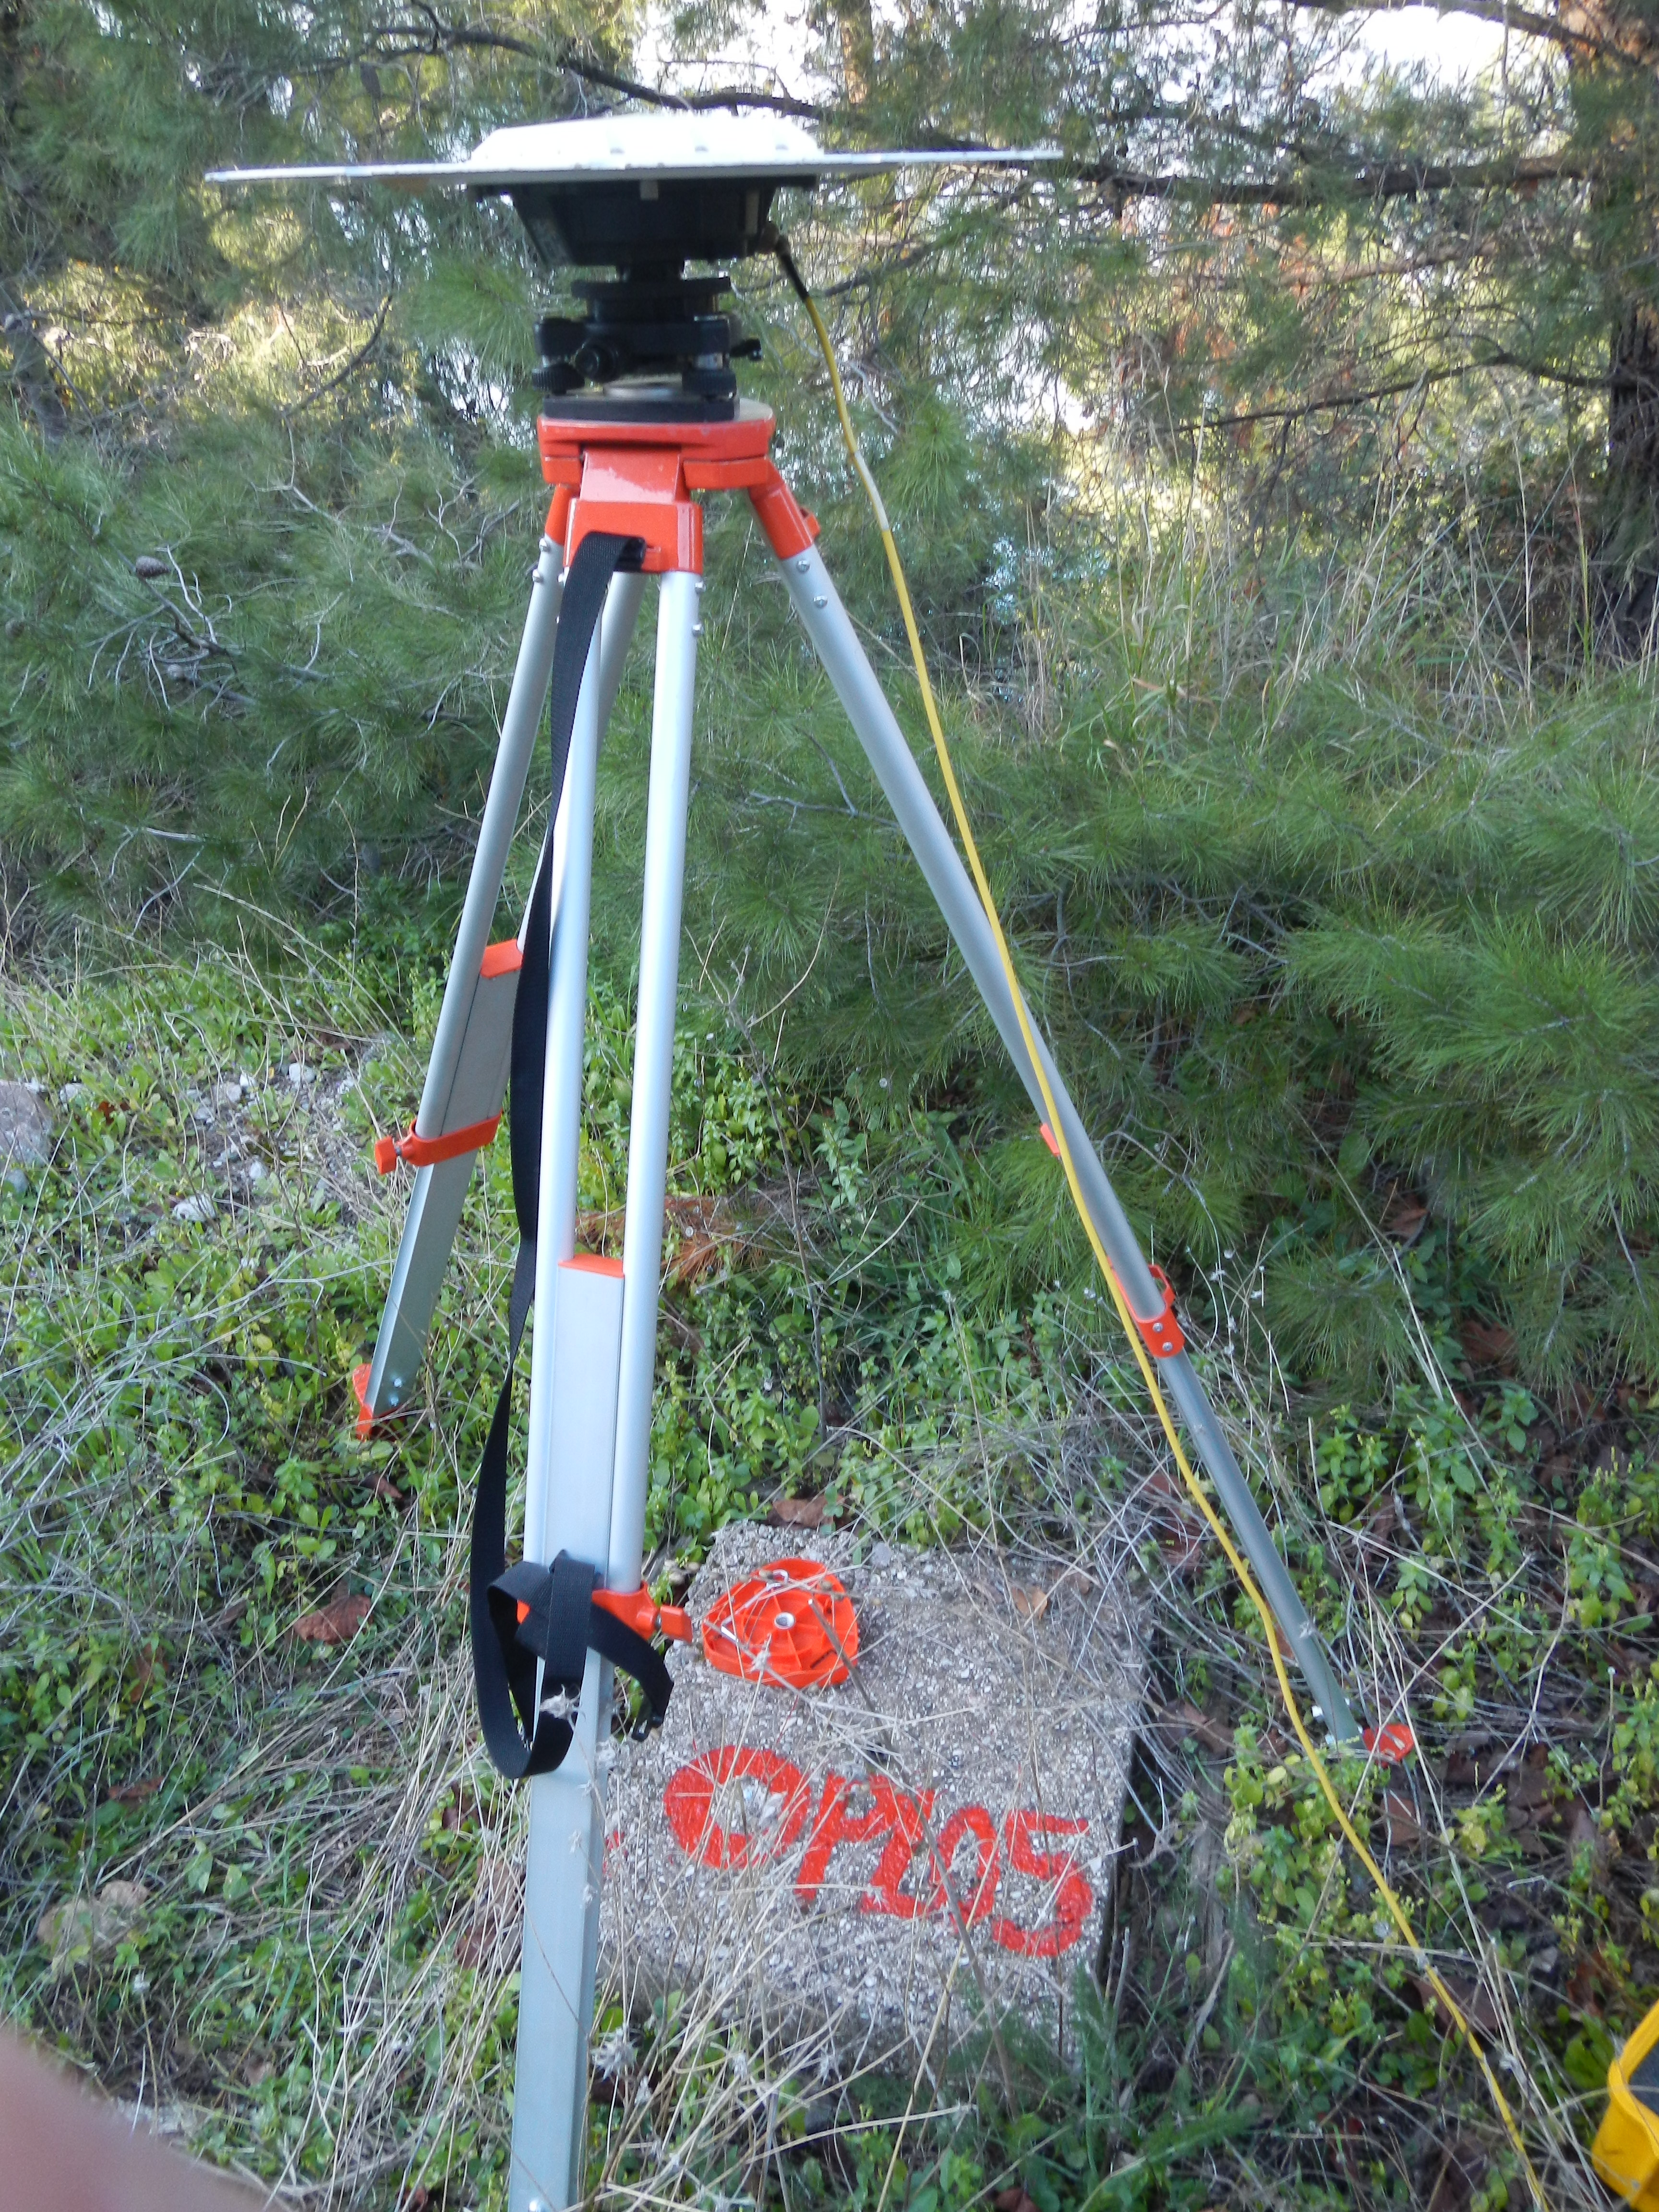
\includegraphics[trim={0cm 0cm 0cm 0cm},clip,width=.55\textwidth]{img/establish01.jpg}
  \vskip -.2cm
 \caption{PL05}
 \label{fig:PL05}
 \end{center}
 \end{figure}  
  }
  {
 \begin{figure}
 \begin{center}
 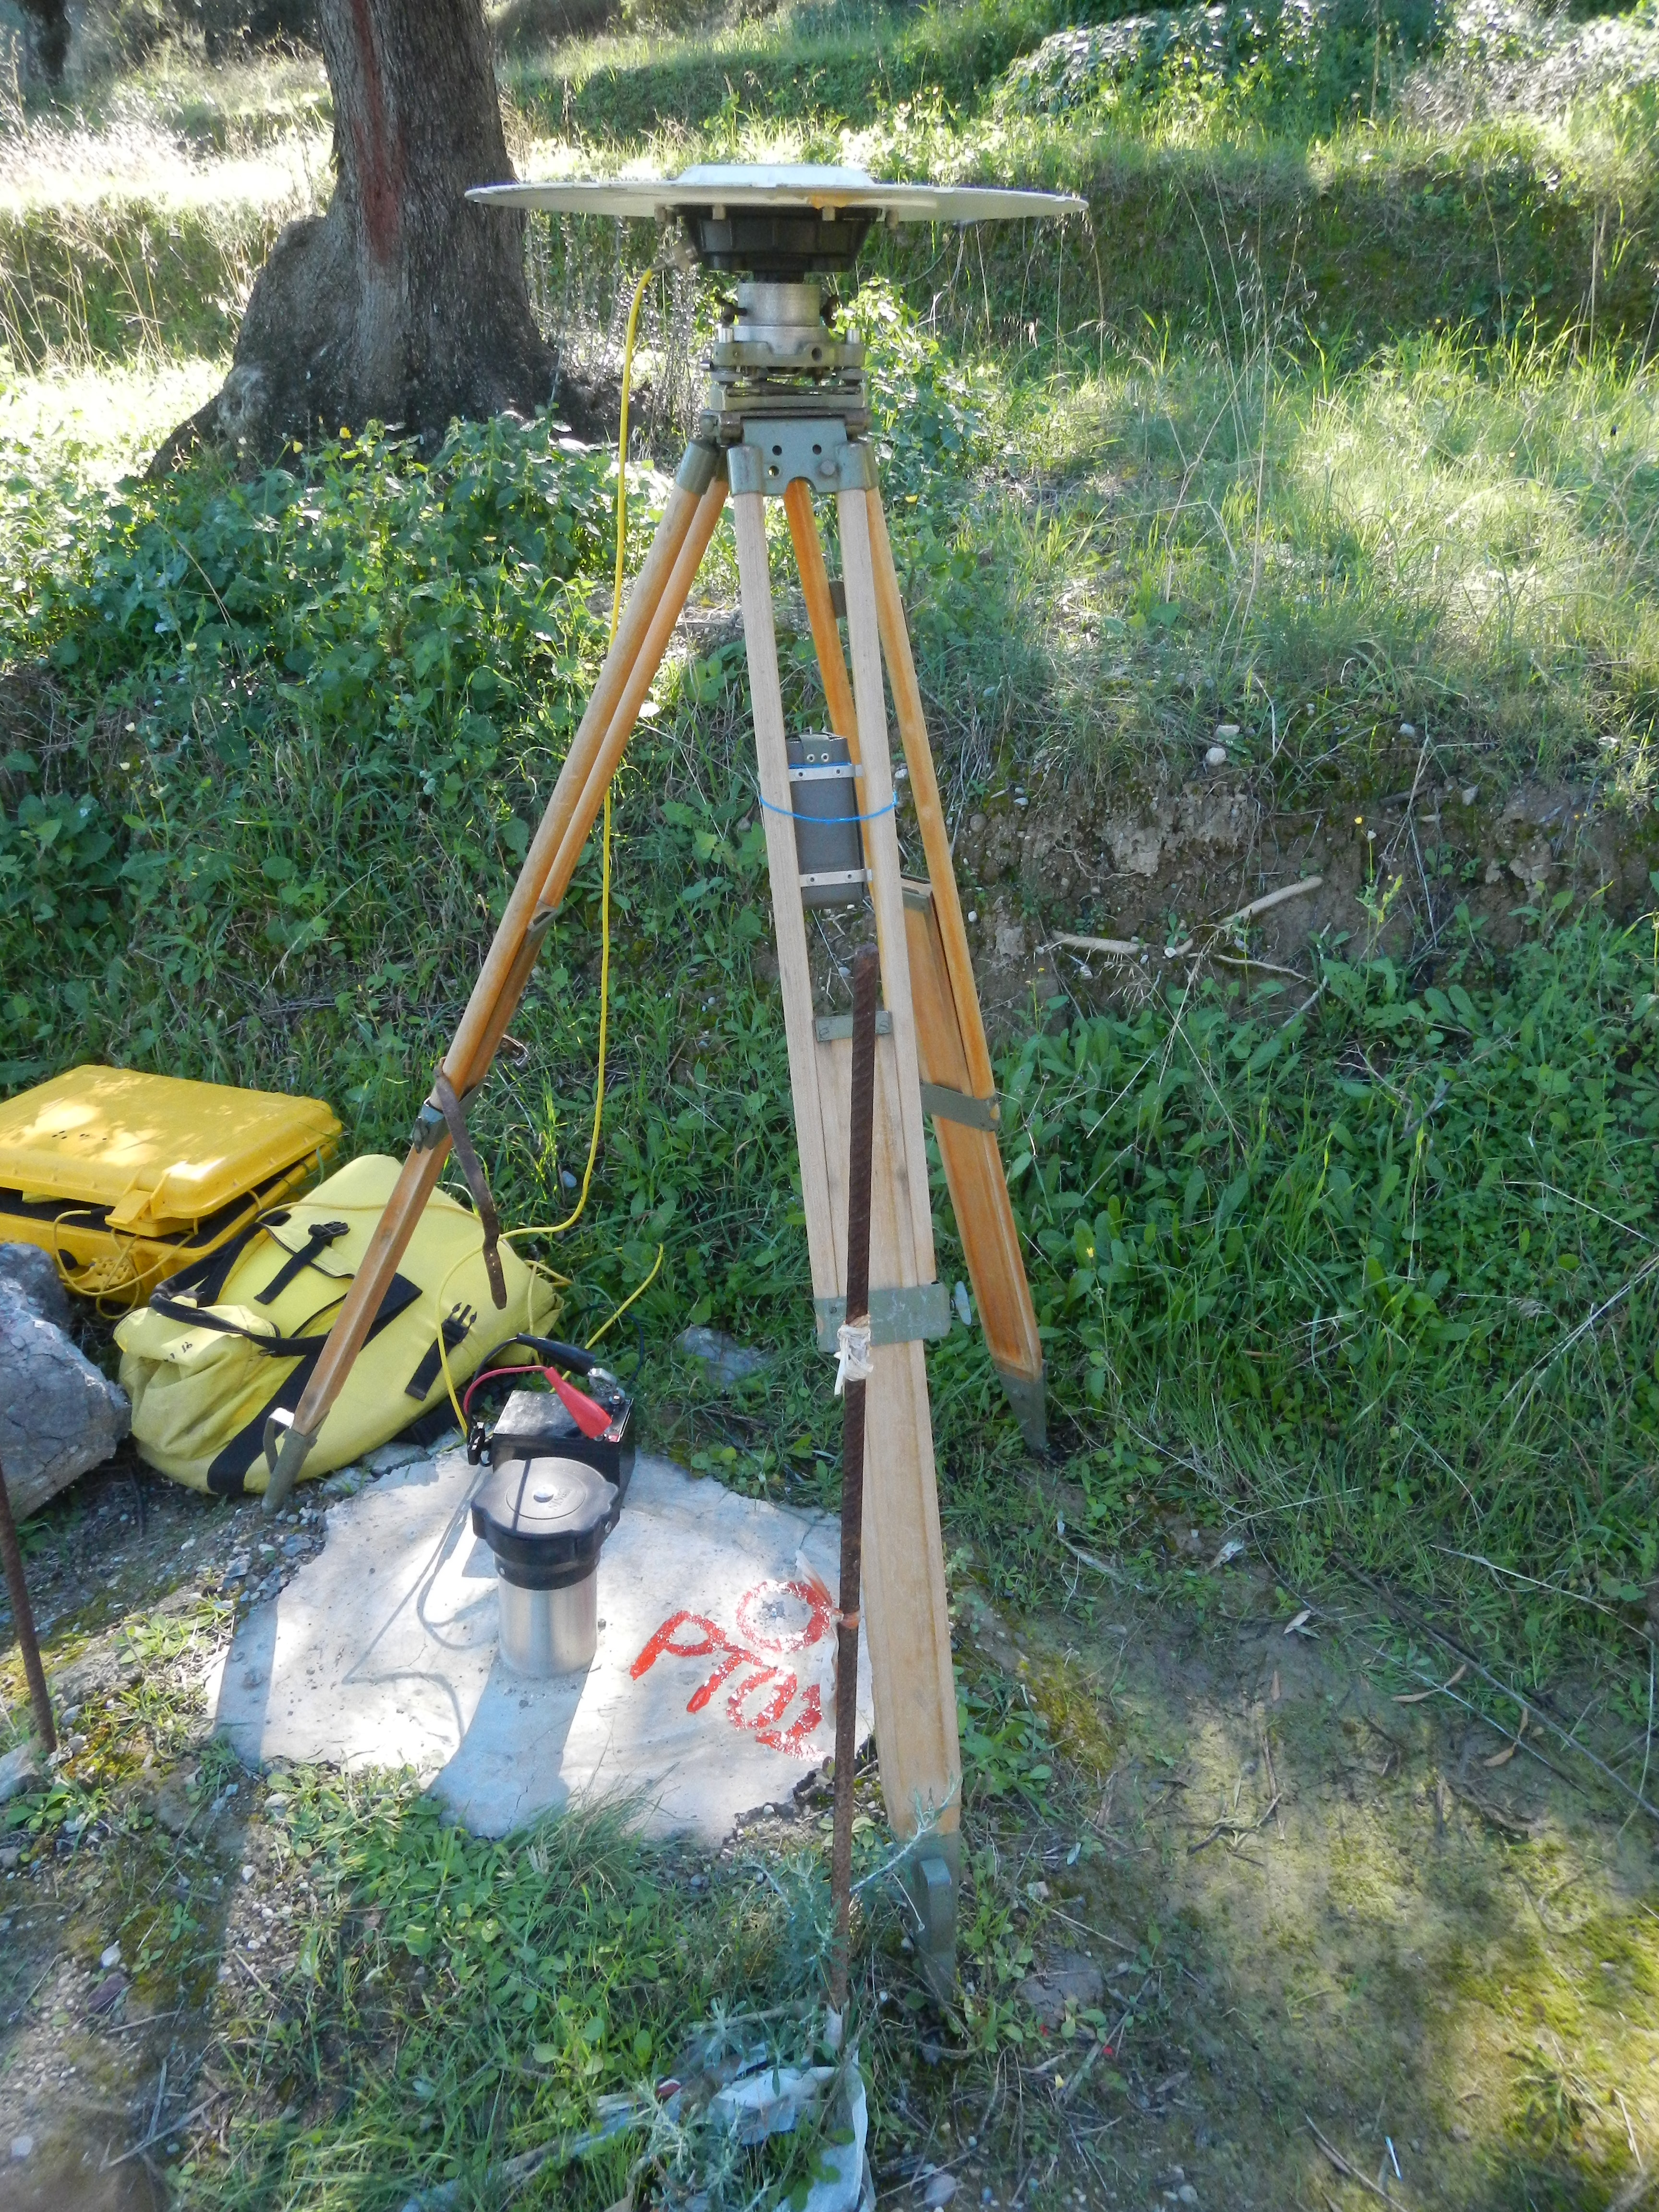
\includegraphics[trim={0cm 0cm 0cm 0cm},clip,width=.55\textwidth]{img/establish02.jpg}
  \vskip -.2cm
 \caption{PT03}
 \label{fig:PT03}
 \end{center}
 \end{figure}
  }
  {
 \begin{figure}
 \begin{center}
 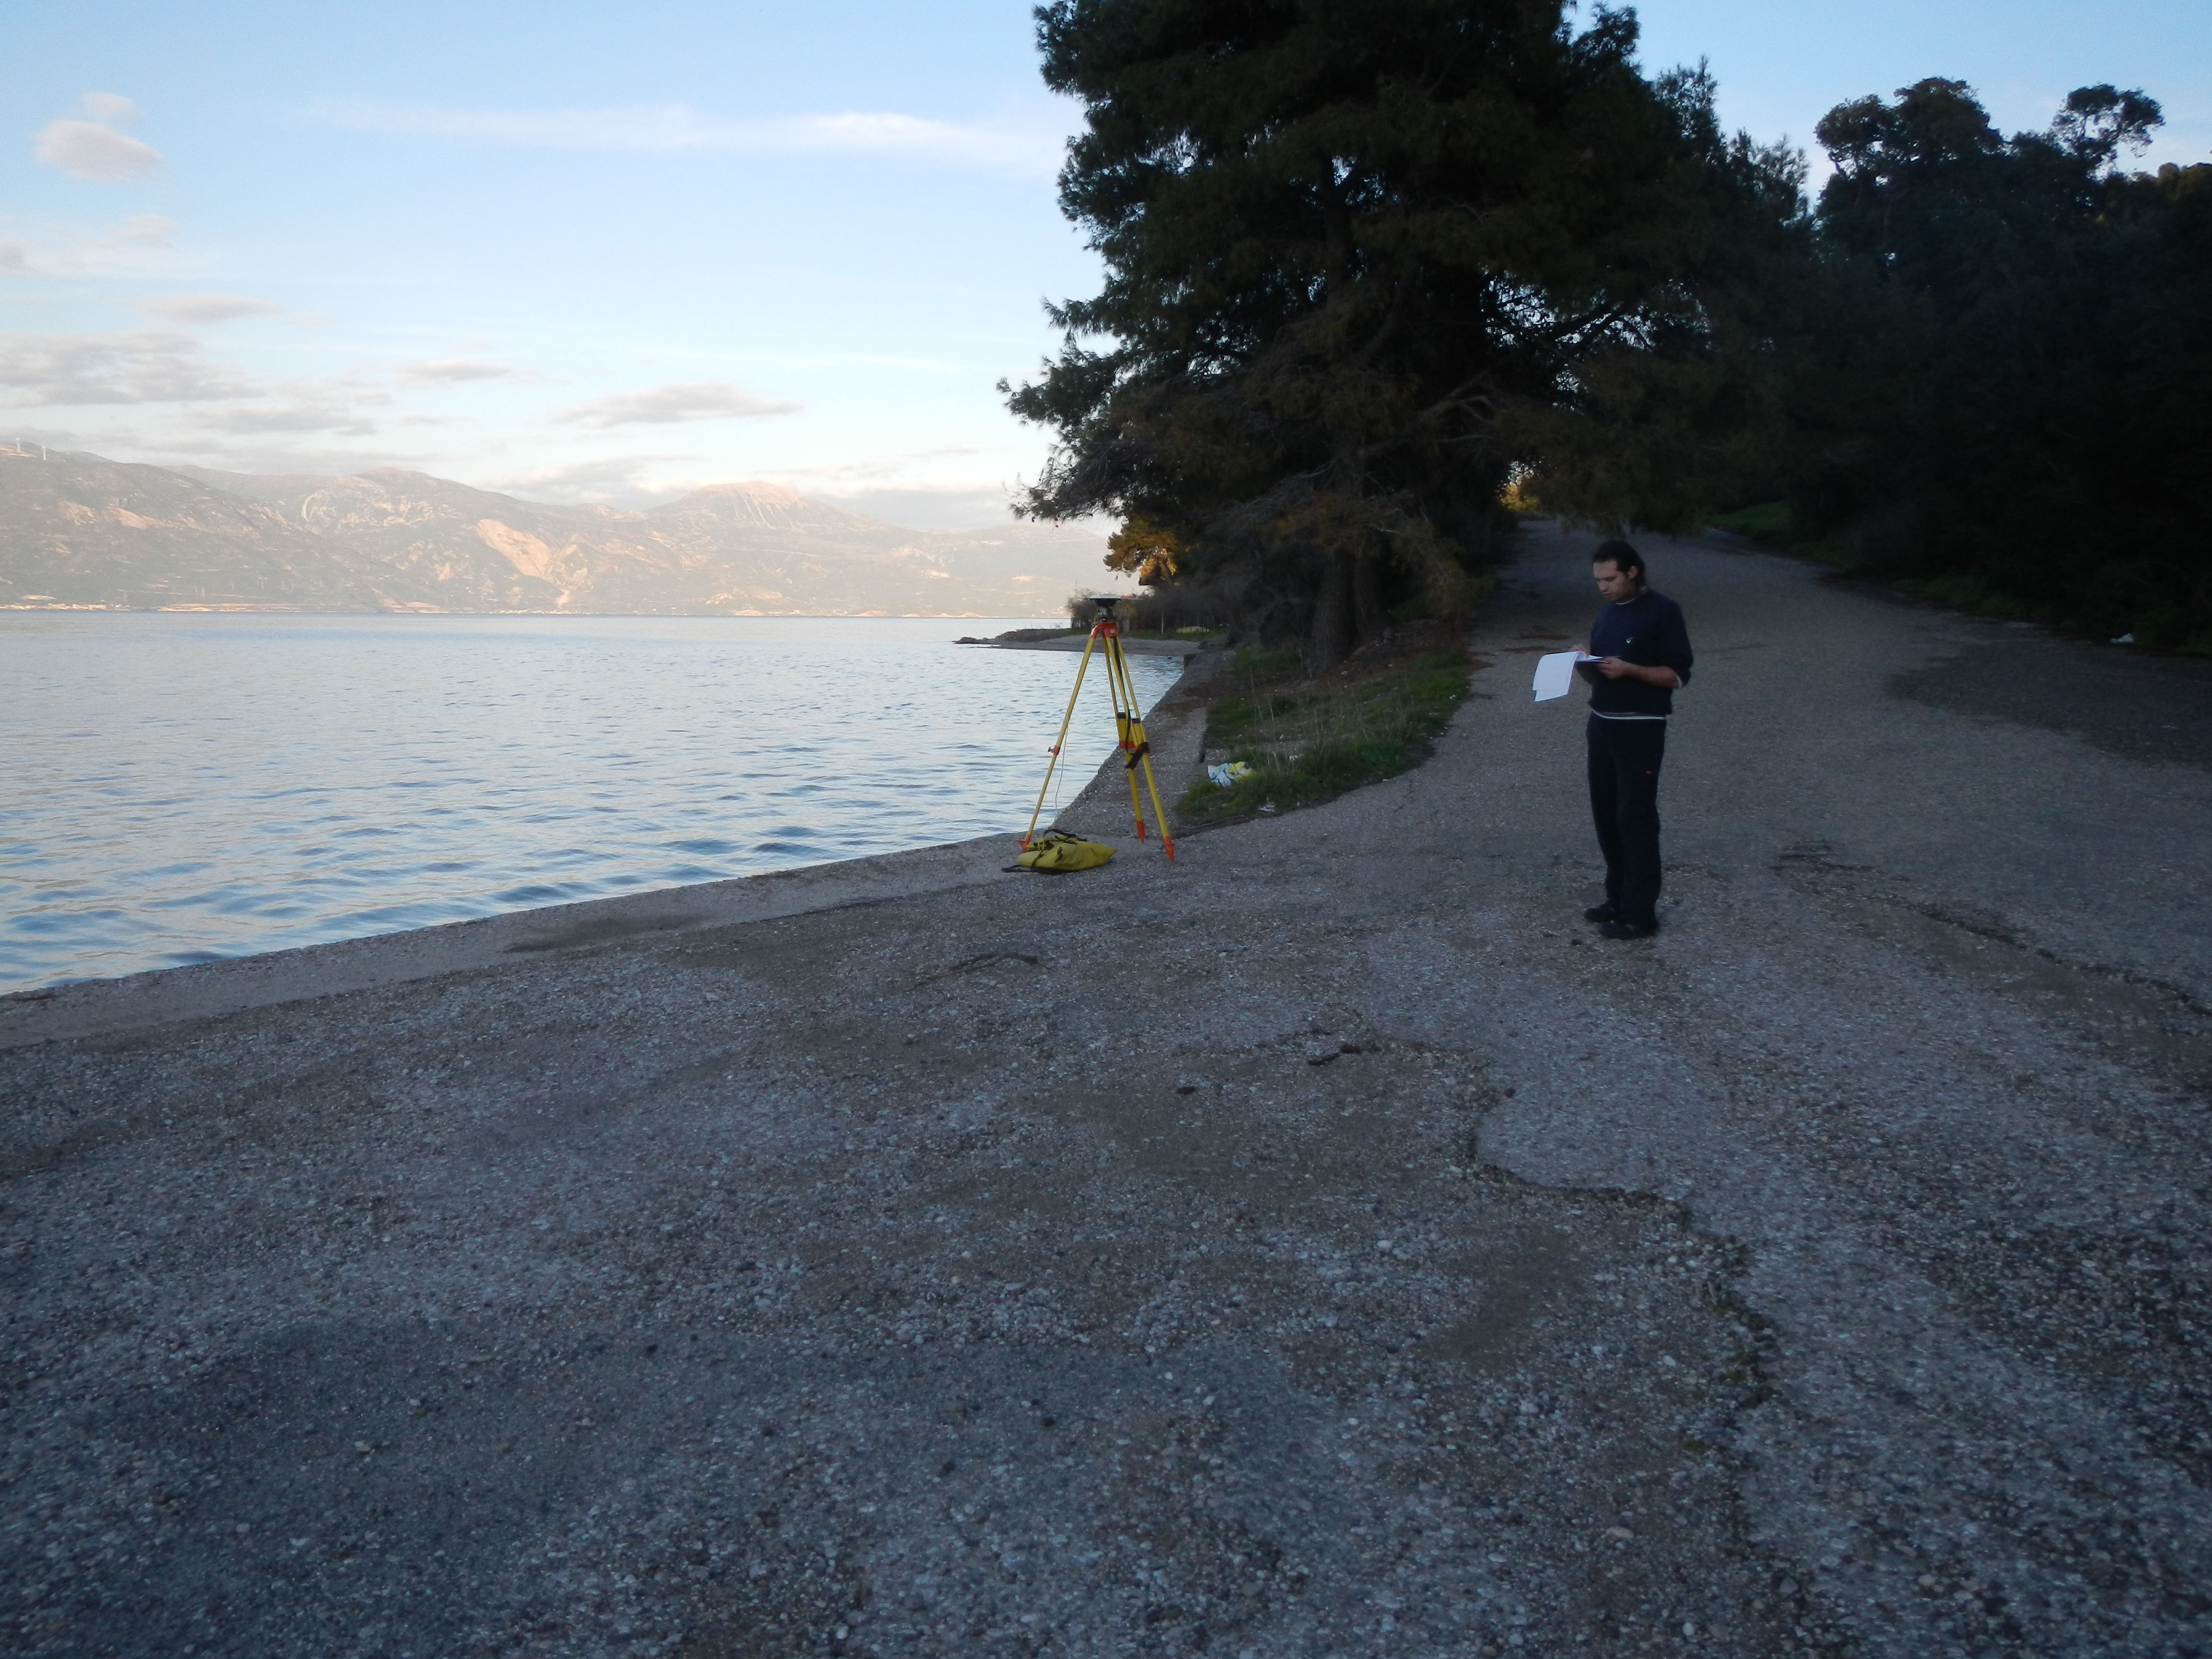
\includegraphics[trim={1cm 2.5cm 1cm 0cm},clip,width=.85\textwidth]{img/N000-photo.jpg}
  \vskip -.2cm
 \caption{N000}
 \label{fig:N000}
 \end{center}
 \end{figure} 
  }
  {
 \begin{figure}
 \begin{center}
 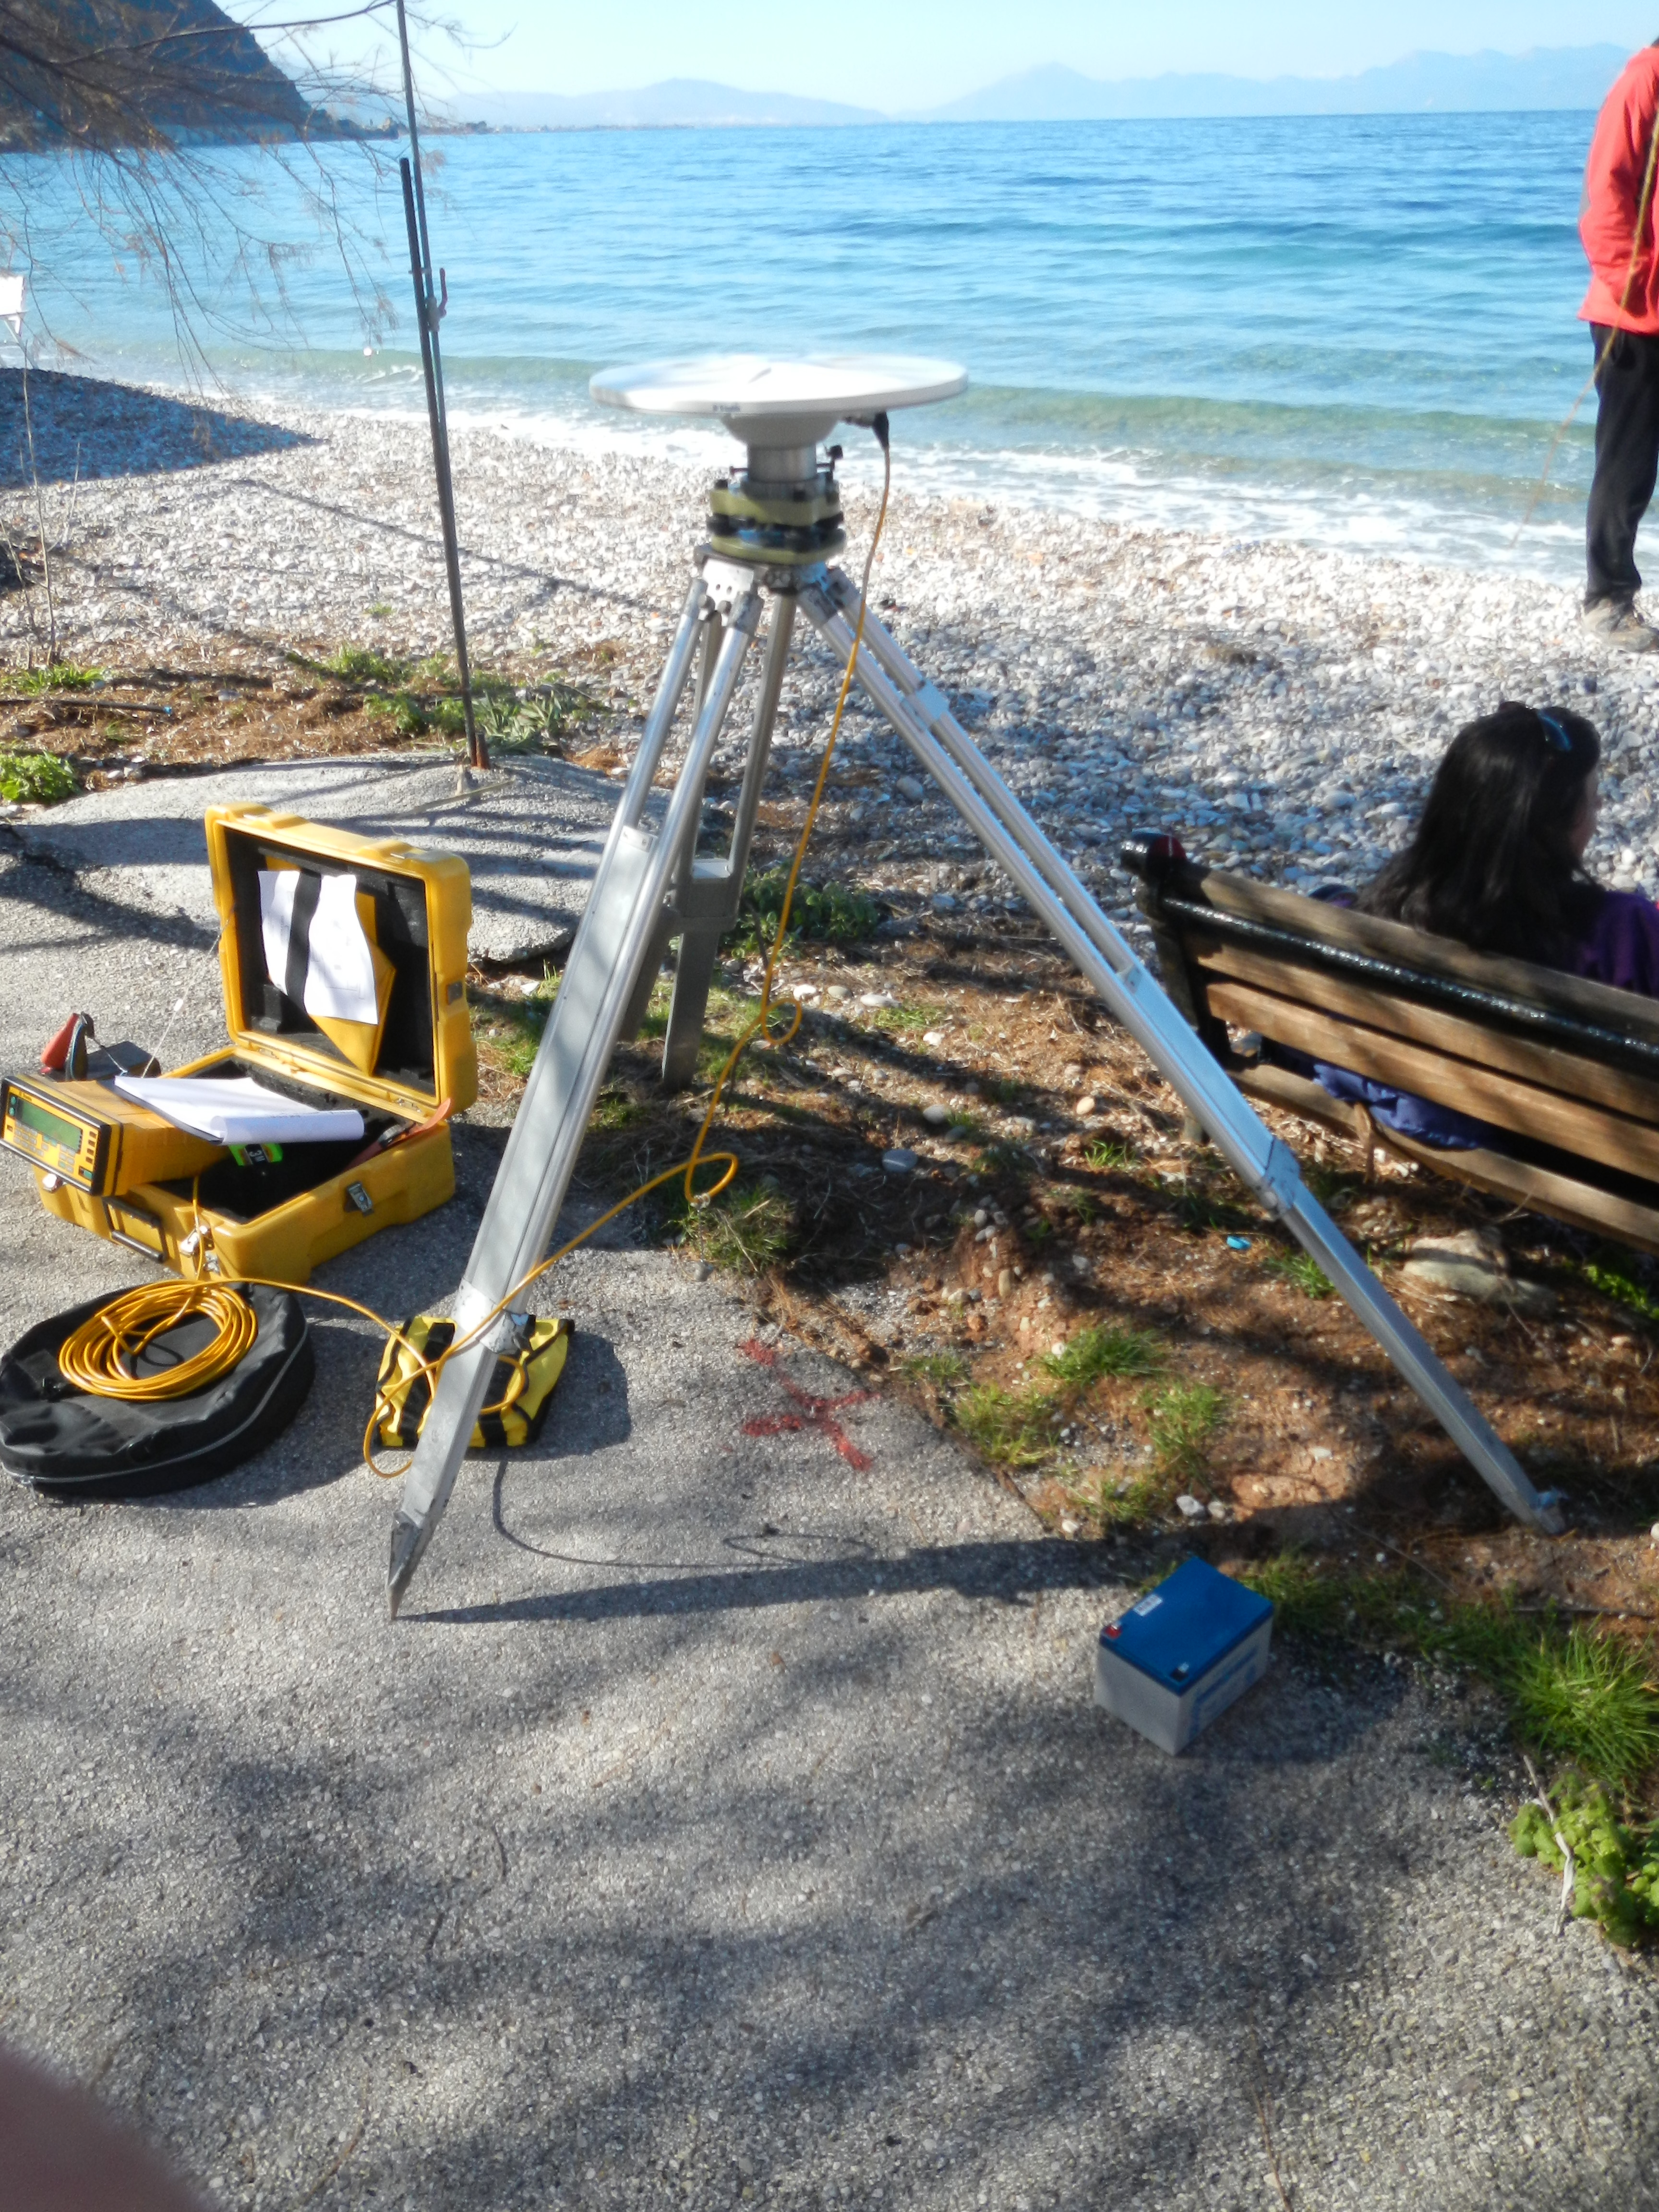
\includegraphics[trim={0cm 3cm 0cm 0cm},clip,width=.55\textwidth]{img/establishpt07.jpg}
  \vskip -.2cm
 \caption{PT07}
 \label{fig:PT07}
 \end{center}
 \end{figure}
  }
\end{frame}

\begin{frame}\frametitle{Υλοποίηση Δικτύου}\framesubtitle{Σκαριφήματα υπαίθρου}
\begin{columns}[T] % align columns
\begin{column}{.5\textwidth}
\begin{figure}
 \begin{center}
 \vskip -.5cm
 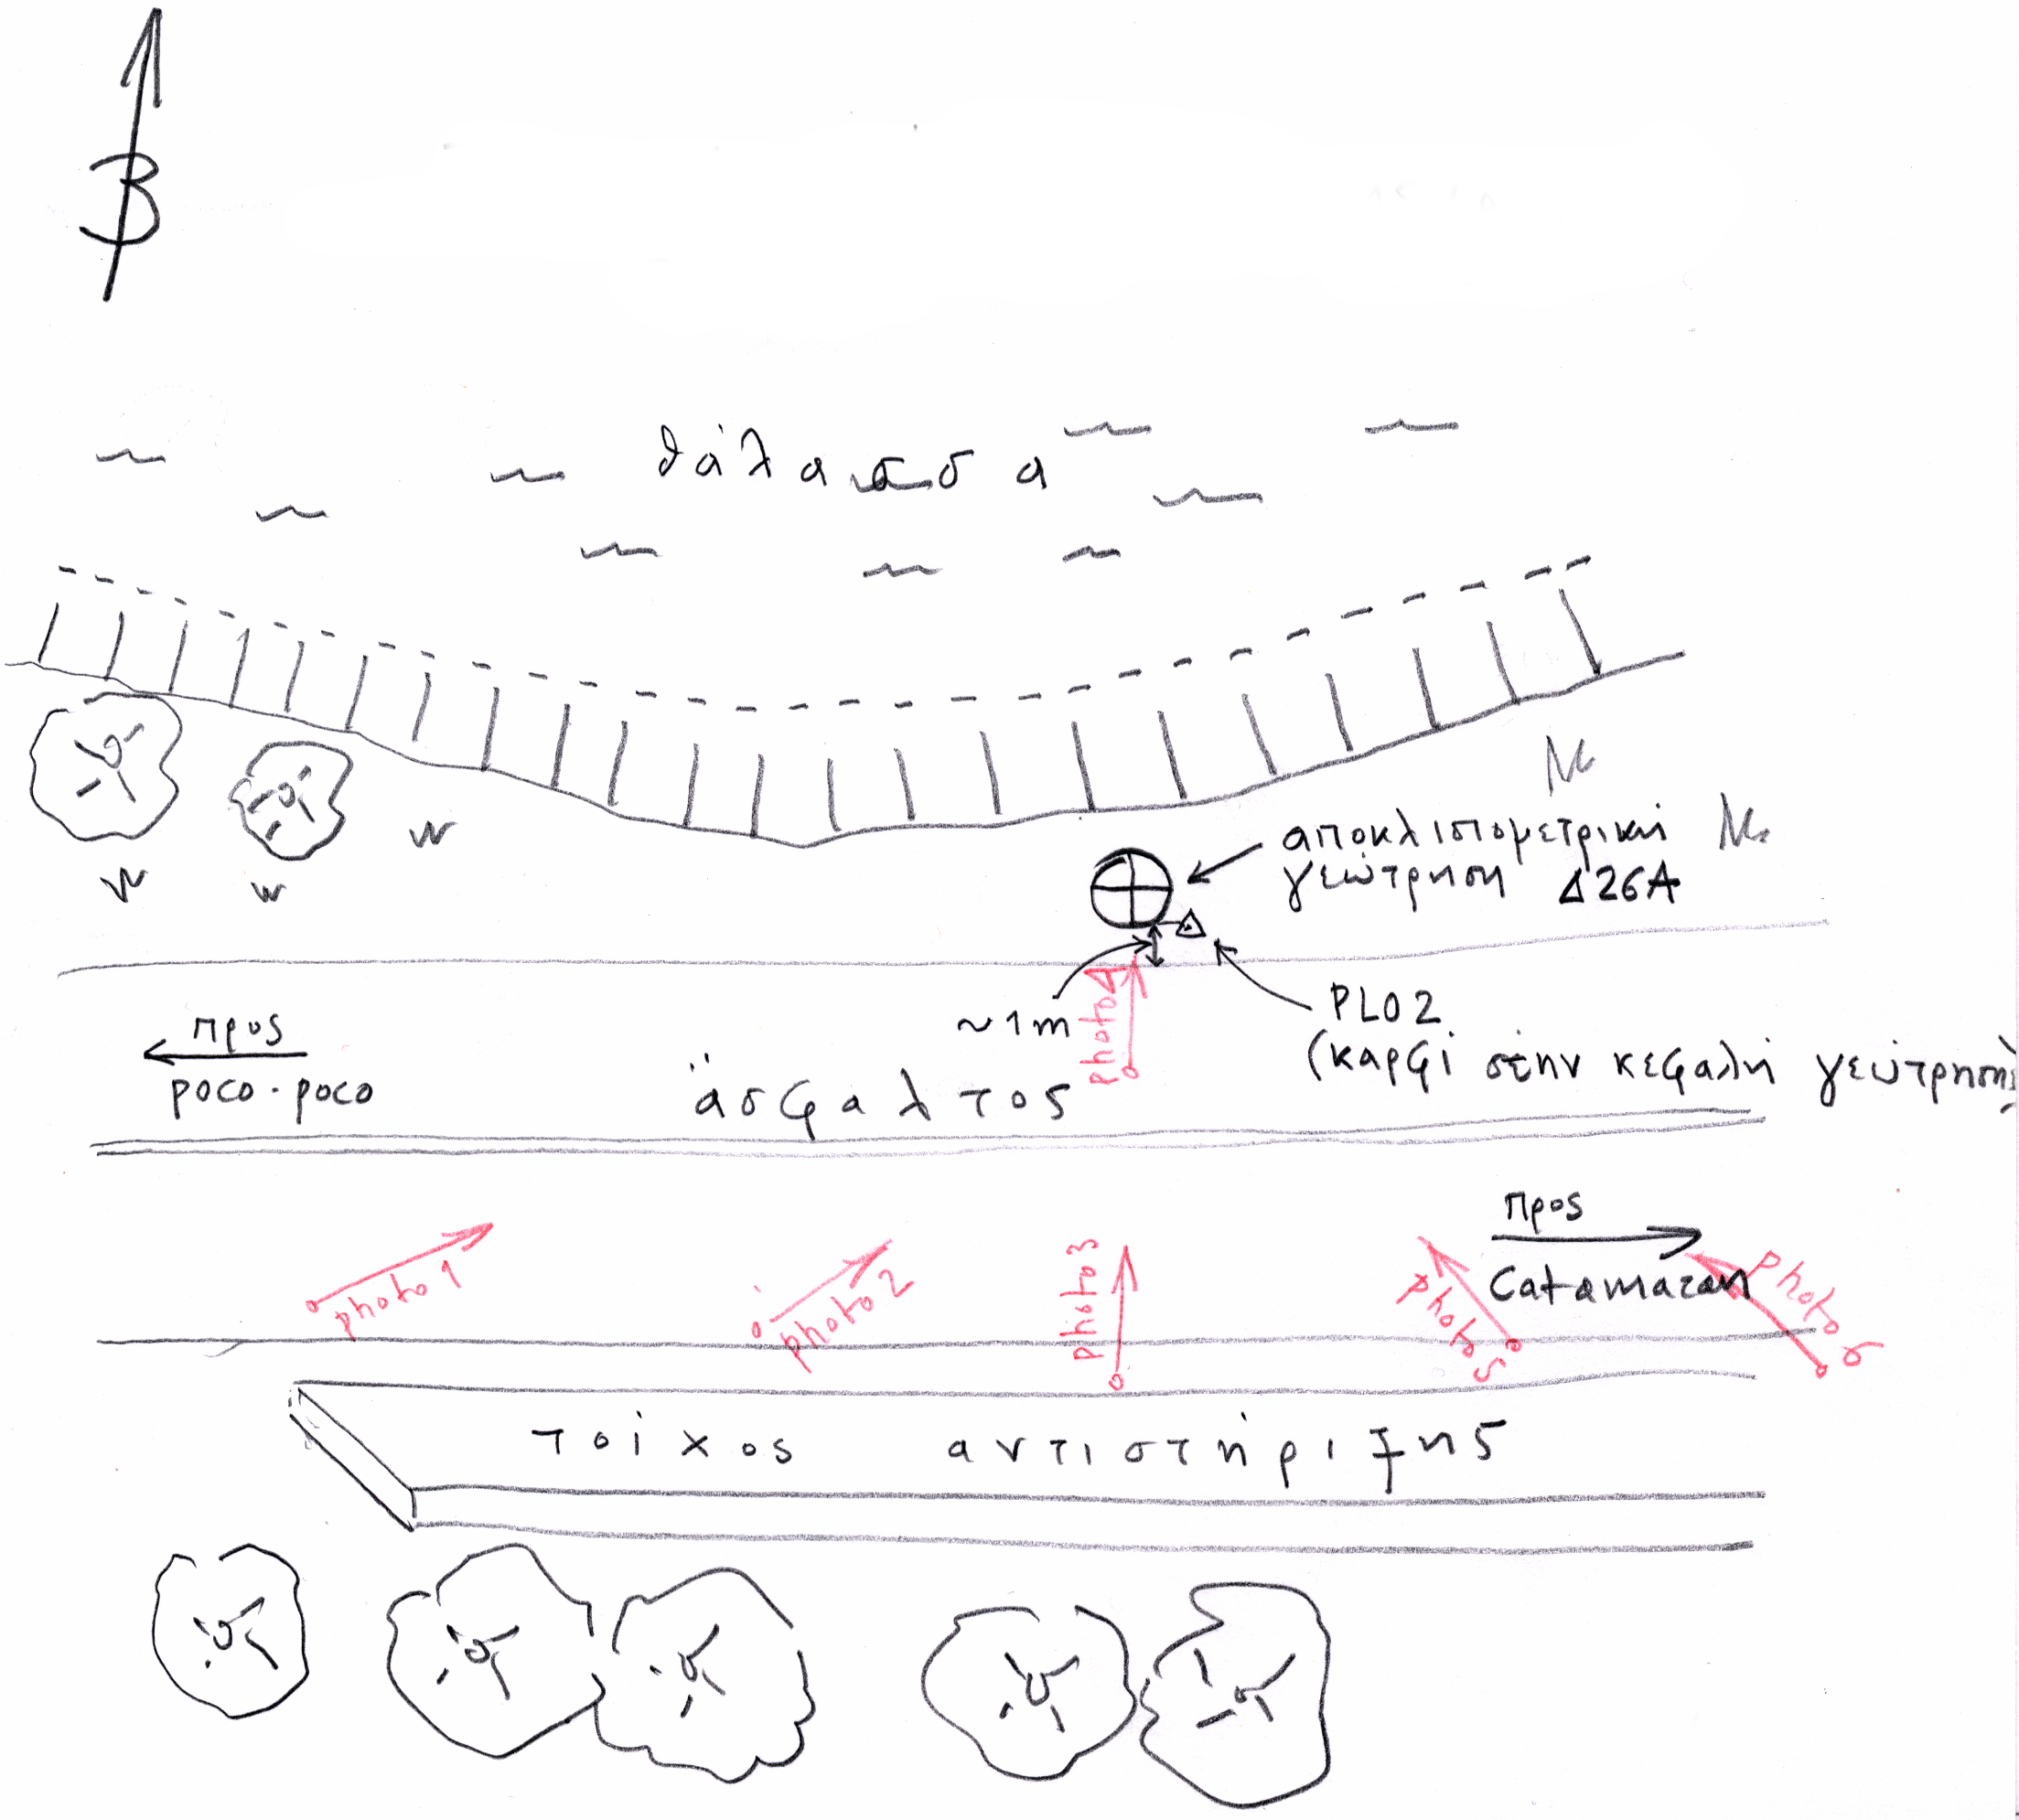
\includegraphics[trim={0cm 0cm 0cm 0cm},clip,width=1\textwidth]{img/skarPL02.png} %1 2.2 0 0
%  \vskip -.7cm
 \caption{}
 \label{fig:skar02}
 \end{center}
 \end{figure}
\end{column}

\begin{column}{.5\textwidth}
\begin{figure}
 \begin{center}
 \vskip -.5cm
 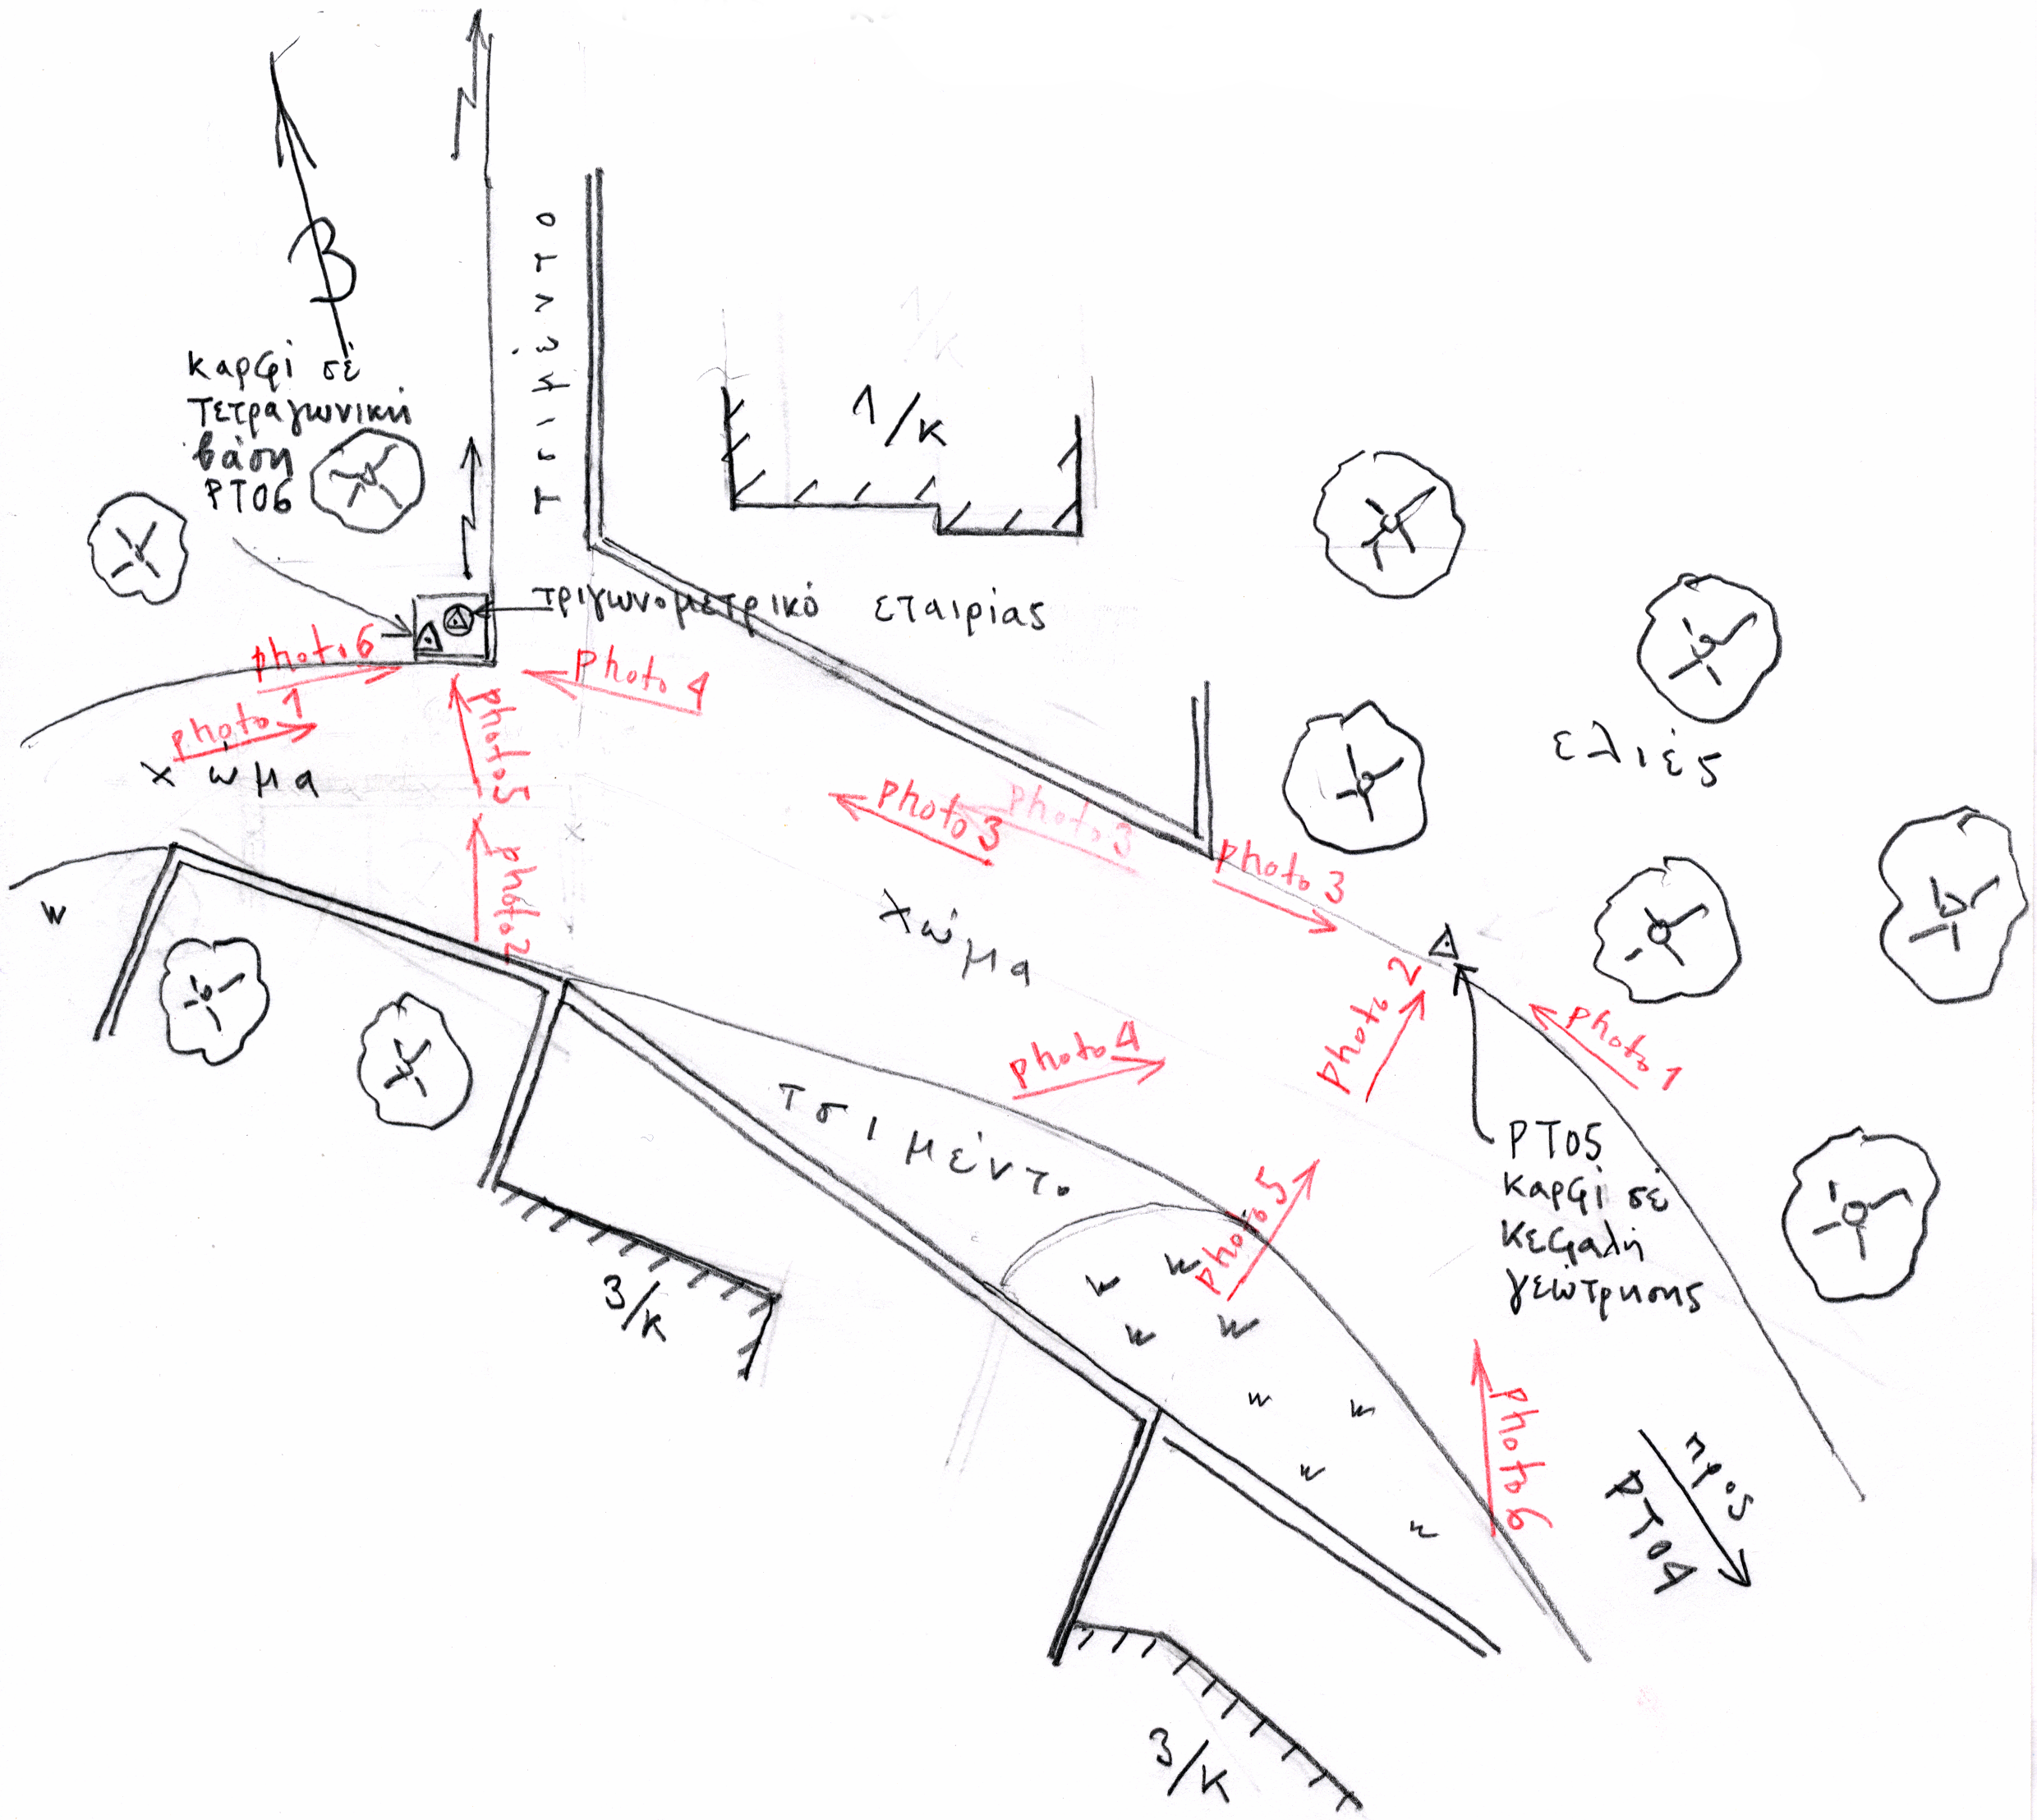
\includegraphics[trim={0cm 0cm 0cm 0cm},clip,width=1\textwidth]{img/skarPT05.png} %1 2.2 0 0
%  \vskip -.7cm
 \caption{}
 \label{fig:skar05}
 \end{center}
 \end{figure}
\end{column}
\end{columns}
\end{frame}

\begin{frame}\frametitle{Περιοχή Παναγοπούλας}\framesubtitle{}
\begin{columns}[T] % align columns
\begin{column}{.3\textwidth}
\begin{itemize}
	 \item 7 σημεία
	 \item Ν000 - υπάρχον από άλλες εργασίες
\end{itemize}
\end{column}

\begin{column}{.7\textwidth}
\begin{figure}
 \begin{center}
 \vskip -.5cm
 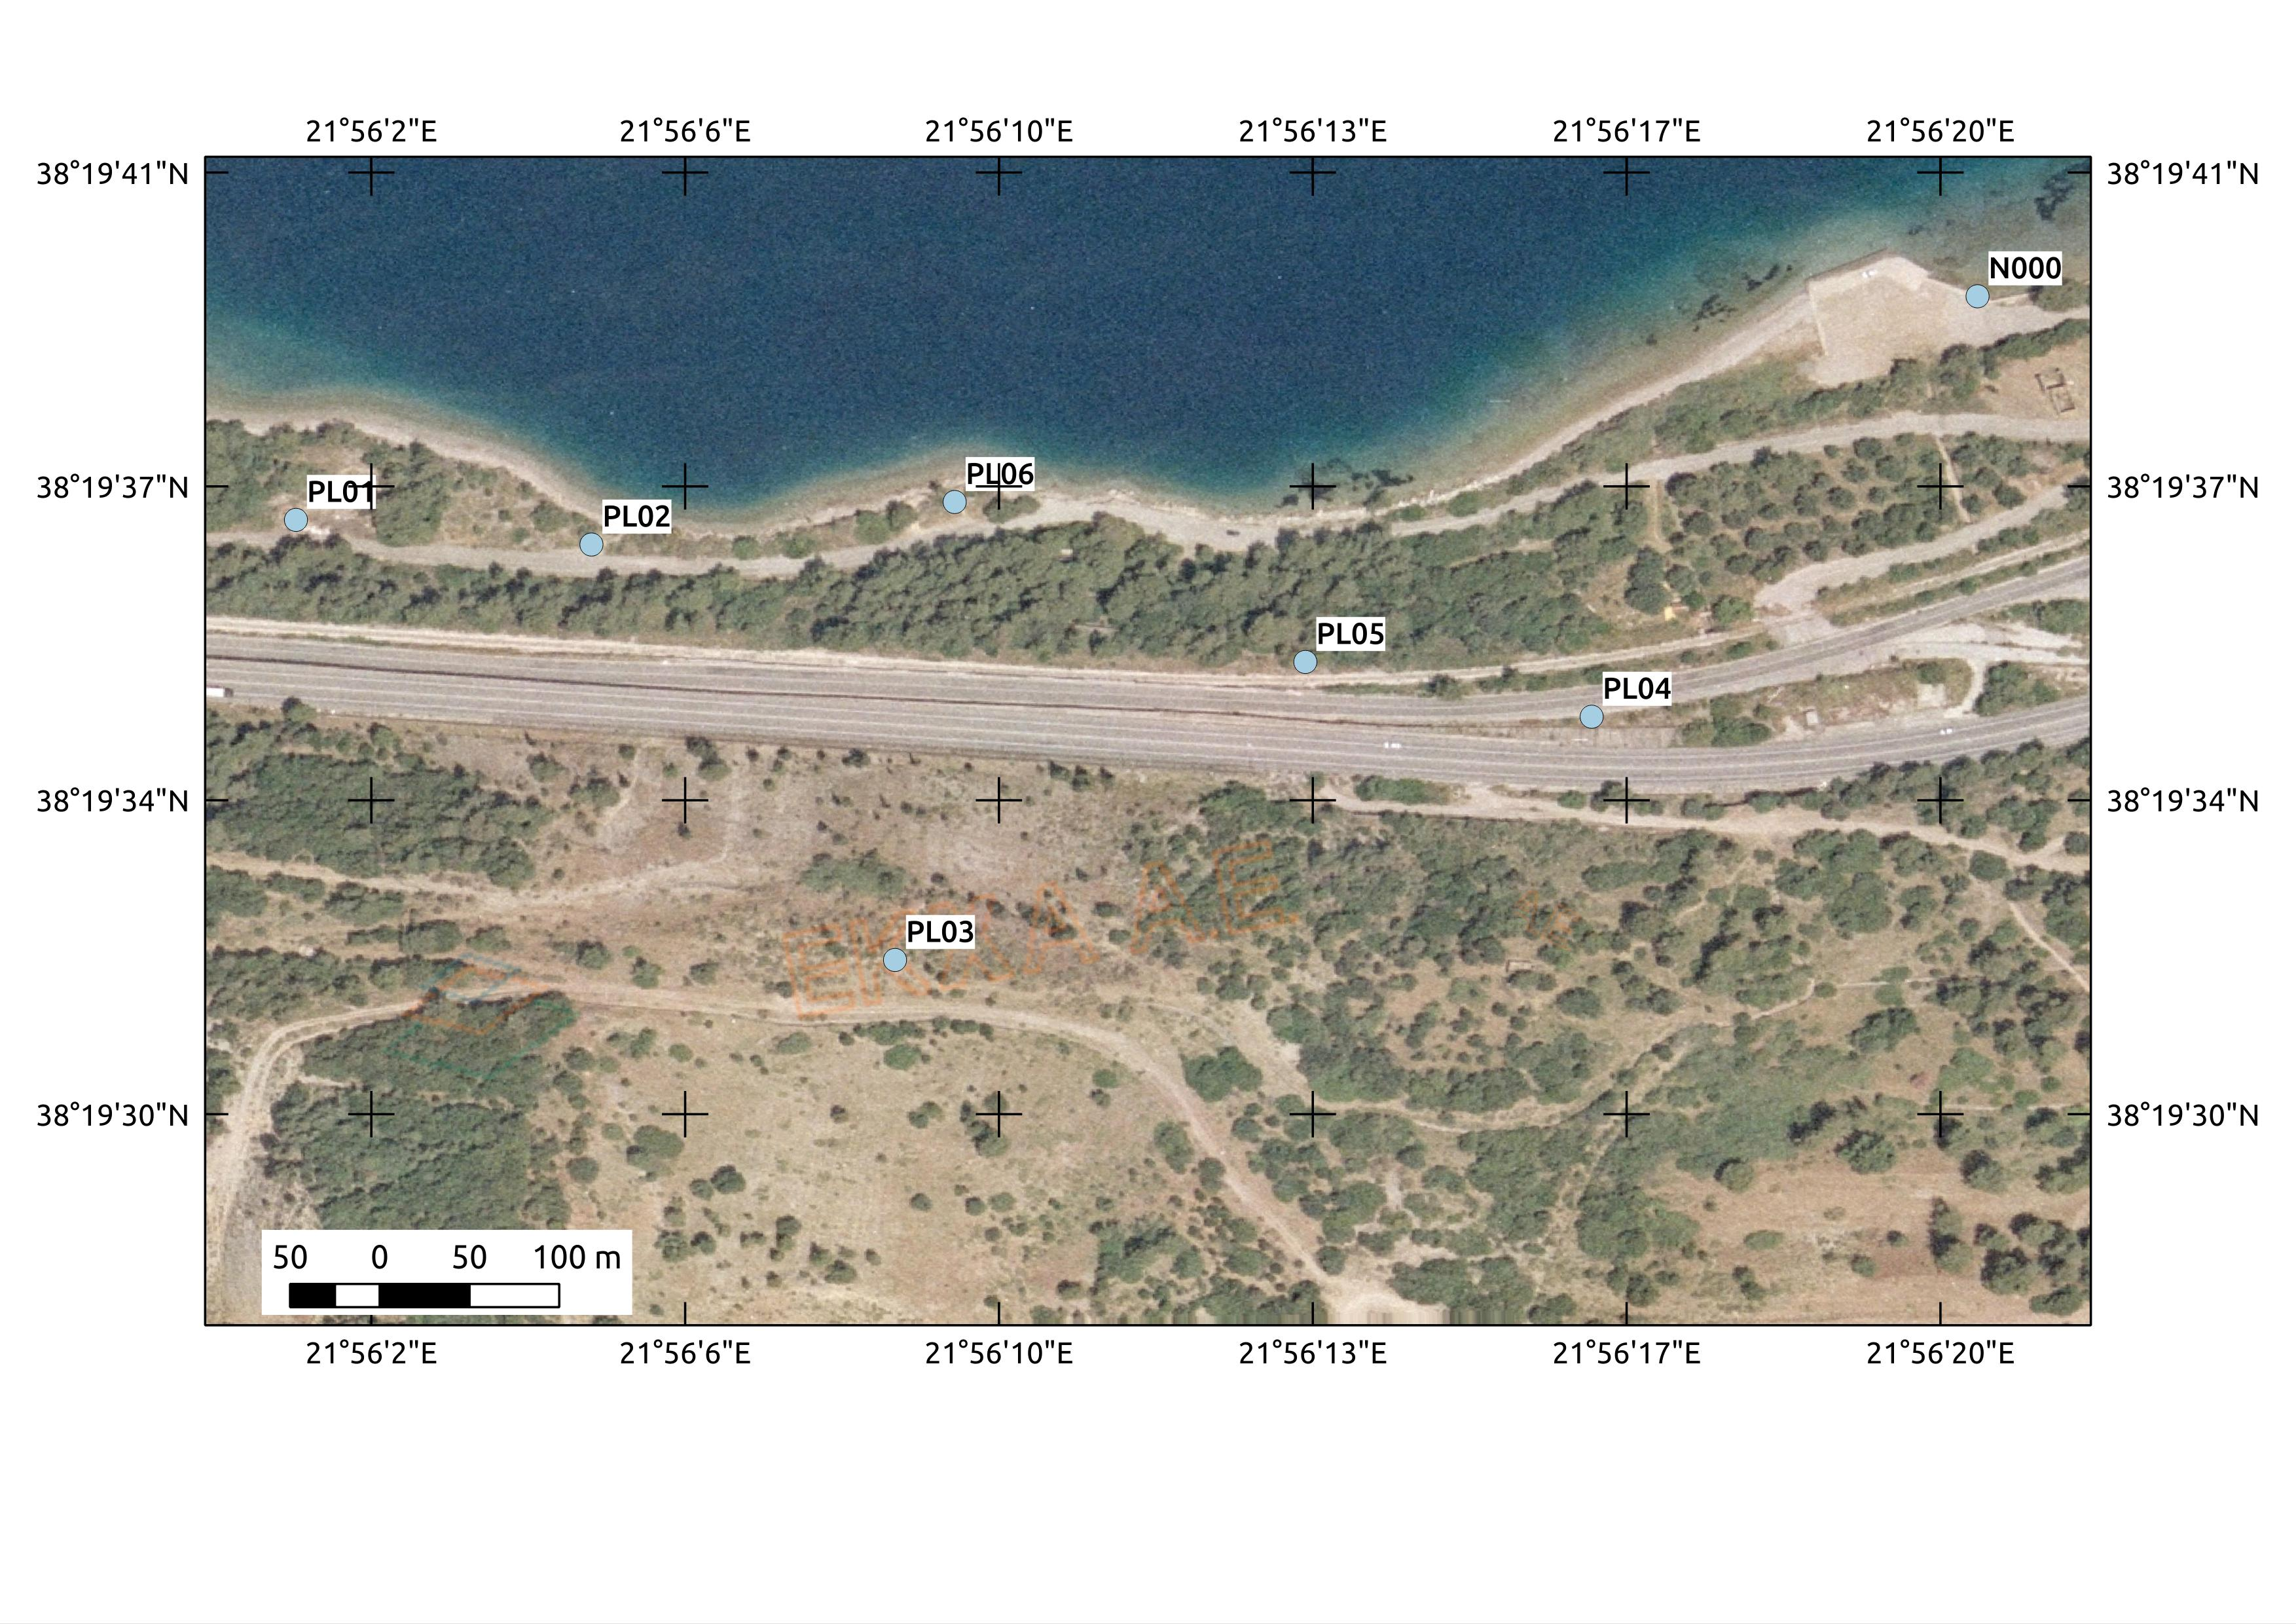
\includegraphics[trim={.4cm 2.5cm .8cm .5cm},clip,width=1\textwidth]{img/panagopoula-net.jpg} %1 2.2 0 0
%  \vskip -.7cm
 \caption{Δίκτυο παρακολούθησης στην περιοχή της Παναγοπούλας}
 \label{fig:plnet}
 \end{center}
 \end{figure}


\end{column}
\end{columns}
\end{frame}

\begin{frame}\frametitle{Περιοχή Πλατάνου}\framesubtitle{}
\begin{columns}[T] % align columns
\begin{column}{.3\textwidth}
\begin{itemize}
	 \item 8 σημεία
	 \item PT07 - εκτός περιοχής κατολίσθησης
\end{itemize}
\end{column}

\begin{column}{.7\textwidth}
\begin{figure}
 \begin{center}
 \vskip -.5cm
 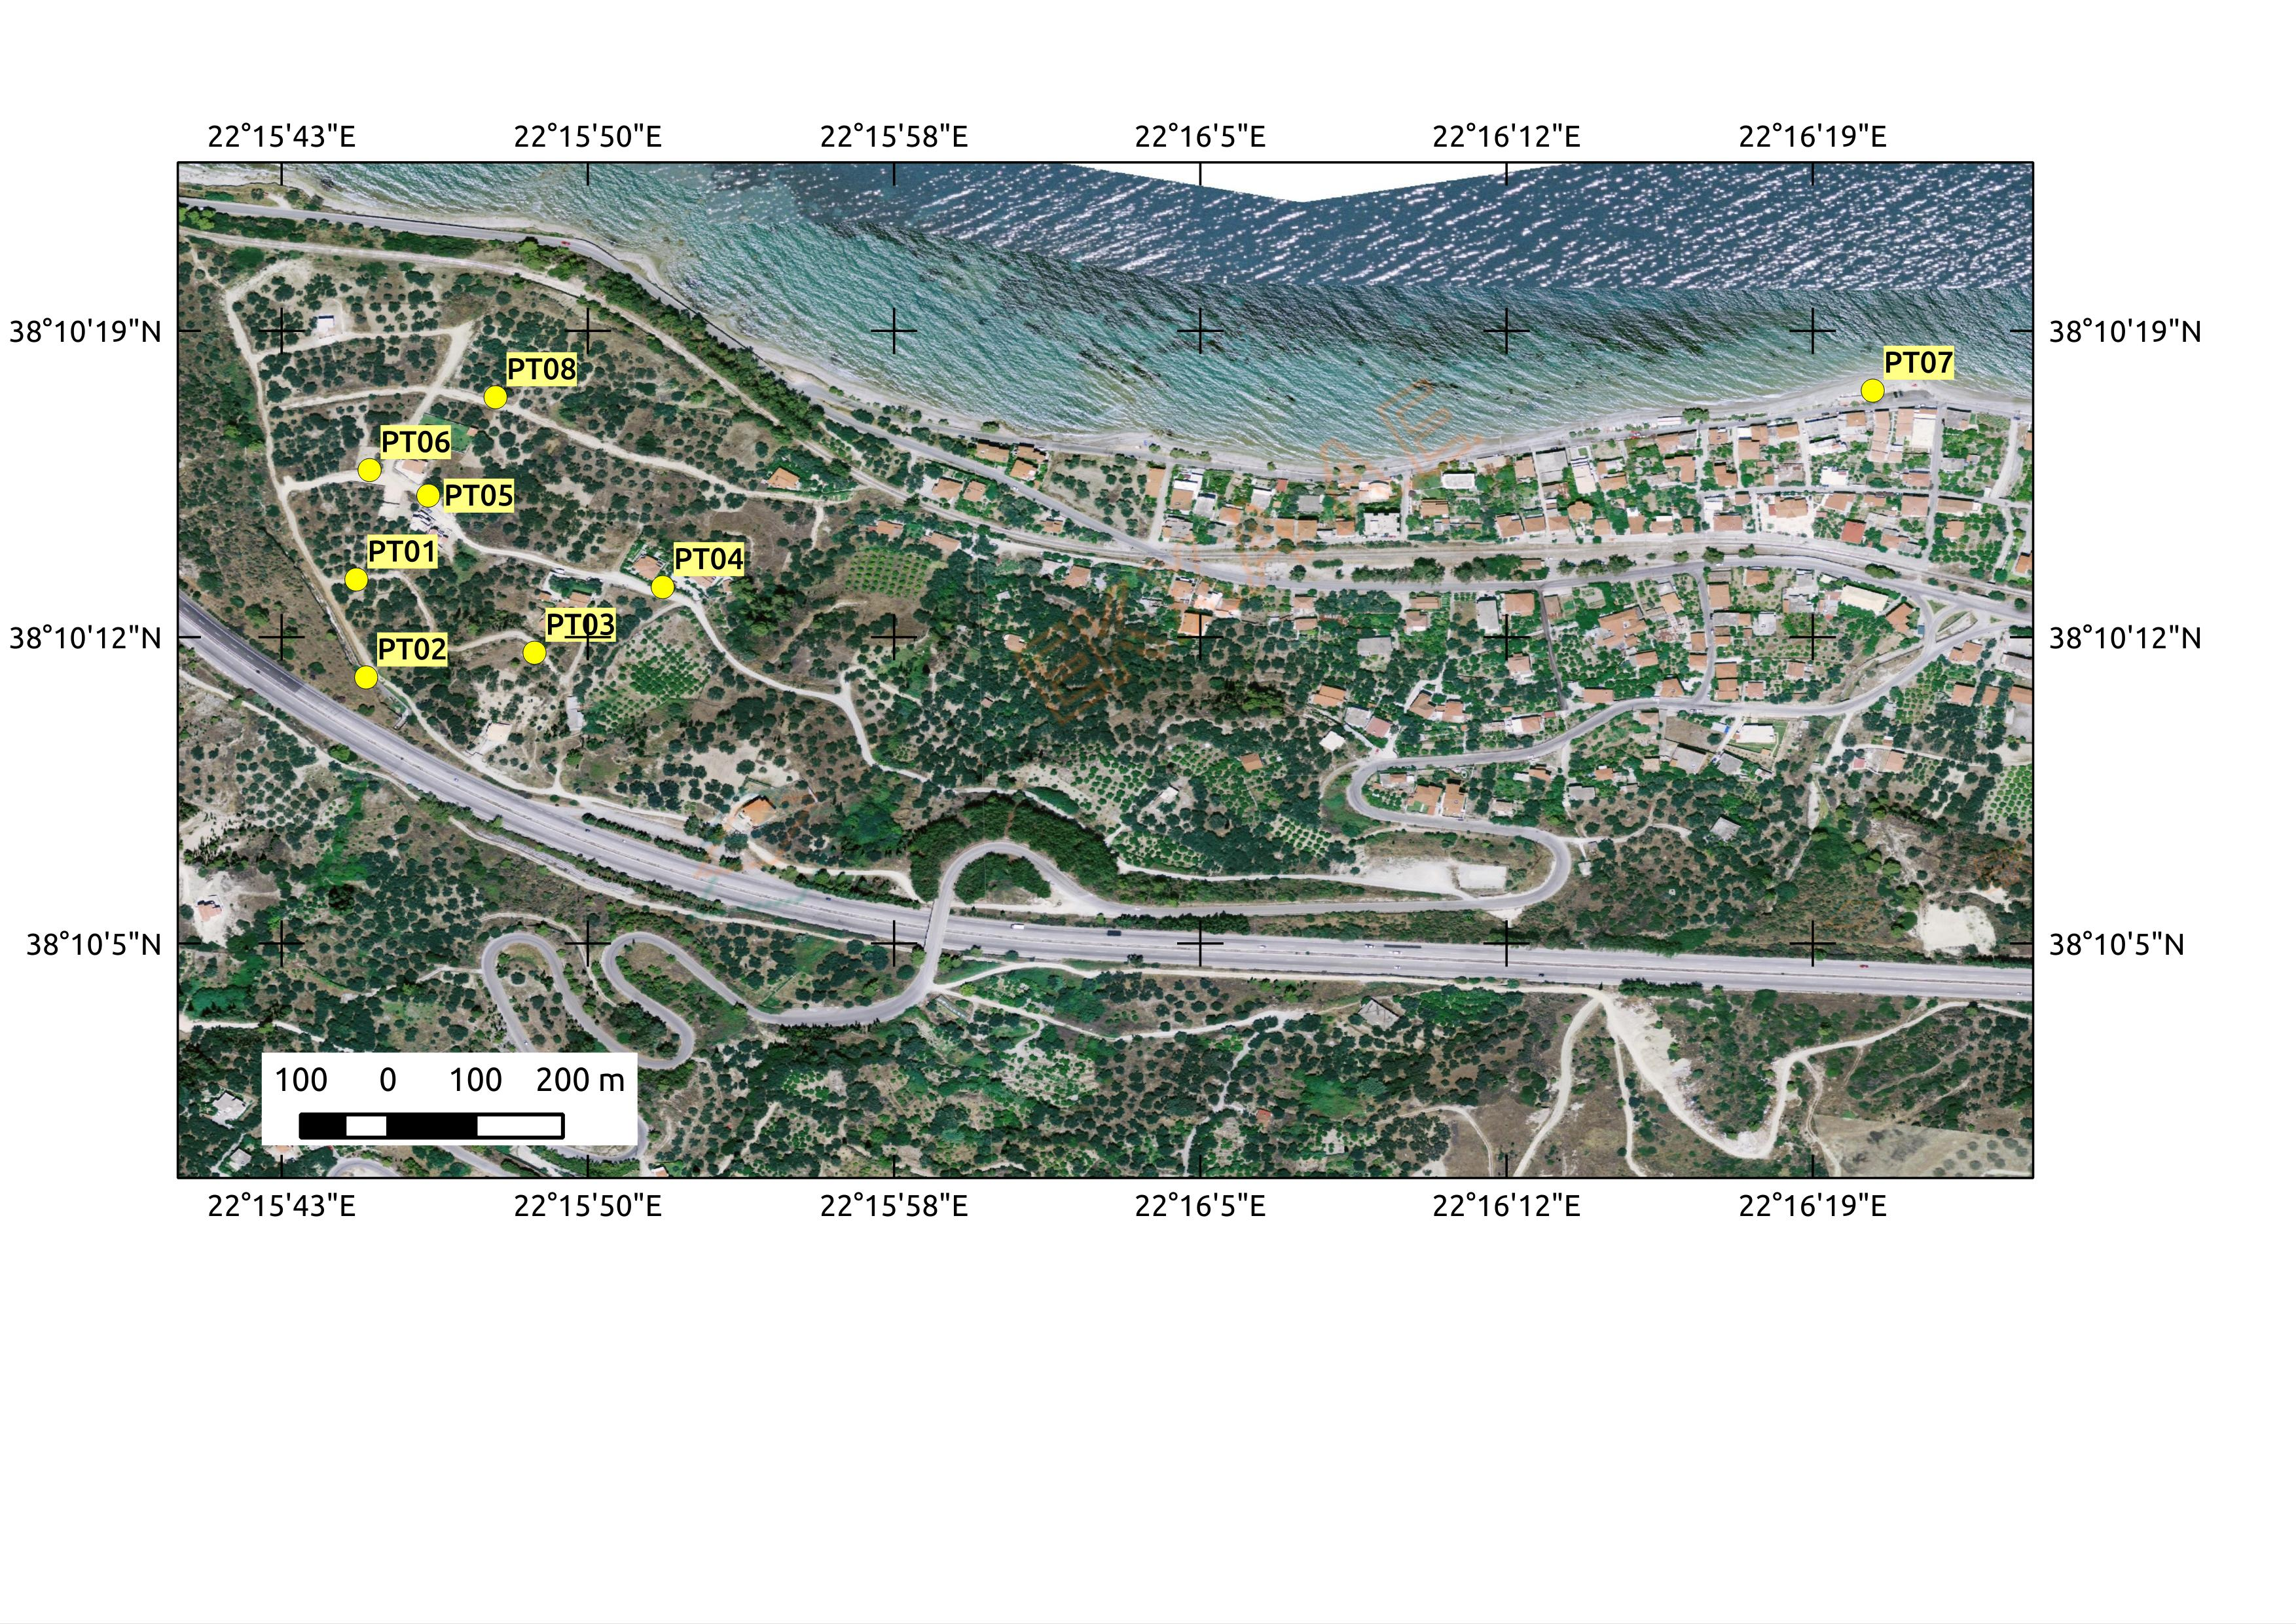
\includegraphics[trim={.3cm 4cm .8cm .5cm},clip,width=1\textwidth]{img/platanos-net.jpg} %1 2.2 0 0
%  \vskip -.7cm
 \caption{Δίκτυο παρακολούθησης στην περιοχή τoυ Πλατάνου}
 \label{fig:ptnet}
 \end{center}
 \end{figure}


\end{column}
\end{columns}
\end{frame}
% 
% \begin{frame}\frametitle{Υλοποίηση Δικτύου}\framesubtitle{}
% \end{frame}

\section{Εργασίες Υπαίθρου}

\begin{frame}\frametitle{Πρότυπο Μετρήσεων Υπαίθρου}\framesubtitle{}
\begin{itemize}
	\item 2 περίοδοι μετρήσεων 2/2015 και 4/2015
	\item 1 σημείο με παρατηρήσεις καθ' όλη τη διάρκεια των μετρήσεων
	\item χρονικό διάστημα μετρήσεων 2 - 3.5 ώρες
	\item διάστημα δηγματοληψίας 15s
	\item γωνία αποκοπής  10 μοίρες
\end{itemize}
\end{frame}

\begin{frame}\frametitle{Εργασίες Υπαίθρου στην Παναγοπούλα}\framesubtitle{}
\begin{table}[]
\caption{1η Περίοδος μετρήσεων 15/2/2014}
\label{tab:plobs01}
% \vskip -.5cm
\centering
\resizebox{\textwidth}{!}{%
\begin{tabular}{{l} | *{3}{l}{c}}
Kωδικός & Κεραία & Δέκτης & Όνομα Αρχείου & Υψος κεραίας (obs) (m) \\
\hline \hline
N000    & TRM33429.00+GP  NONE & TRM4700 & N0000460.14o & 1.6317 \\
PL01    & TRM22020.00+GP  NONE & TRM4000SSI & PL010460.14o & 1.3340 \\
PL02    & TRM33429.00+GP  NONE & TRM4700    & PL020460.14o & 1.4730 \\
PL03    & TRM41249.00     NONE & TRM4000SSI & PL030460.14o & 1.5263\\
PL04    & TRM22020.00+GP  NONE & TRM4000SSI & PL040460.14o & 1.3997\\
PL05    & TRM33429.00+GP  NONE & TRM4700    & PL050460.14o & 1.3240 \\
PL06    & TRM41249.00     NONE & TRM4000SSI & PL060460.14o & 1.2903 \\
\hline
\end{tabular}
}
\end{table}
 


\begin{table}[]
\caption{2η Περίοδος μετρήσεων 28/4/2015}
\label{tab:plobs02}
% \vskip -.5cm
\centering
\resizebox{\textwidth}{!}{%
\begin{tabular}{{l} | *{3}{l}{c}}
Kωδικός & Κεραία & Δέκτης & Όνομα Αρχείου & Υψος κεραίας (obs) (m) \\
\hline \hline
N000   & TRM41249.00     NONE & TRM4000SSI & N0001180.15o & 1.3750 \\
PL01   & TRM33429.00+GP  NONE & TRM4700    & PL011180.15o & 1.3620 \\
PL02   & TRM33429.00+GP  NONE & TRM4700    & PL021180.15o & 1.3010 \\
PL03   & TRM33429.00+GP  NONE & TRM4700    & PL031180.15o & 1.3250 \\
PL04   & TRM33429.00+GP  NONE & TRM4700    & PL041180.15o & 1.4060 \\
PL05   & TRM22020.00+GP  NONE & TRM4000SSI & PL051180.15o & 1.2408 \\
PL06   & TRM22020.00+GP  NONE & TRM4000SSI & PL061180.15o & 1.0830 \\
\hline
\end{tabular}
}
\end{table}


\end{frame}

\begin{frame}\frametitle{Εργασίες Υπαίθρου στον Πλάτανο}\framesubtitle{}

\begin{table}[]
\caption{1η Περίοδος μετρήσεων 16/2/2014}
\label{tab:ptobs01}
\centering
\resizebox{\textwidth}{!}{%
\begin{tabular}{{l} | *{3}{l}{c}}
Kωδικός & Κεραία & Δέκτης & Όνομα Αρχείου & Υψος κεραίας (obs) (m) \\
\hline \hline
PT01    & TRM33429.00+GP  NONE & TRM4700 & PT010470.14o & 1.3883 \\
PT02    & TRM33429.00+GP  NONE & TRM4700 & PT020470.14o & 1.4487 \\
PT03    & TRM22020.00+GP  NONE & TRM4000SSI & PT030470.14o & 1.5357 \\
PT04    & TRM33429.00+GP  NONE & TRM4700  & PT040470.14o & 1.3743 \\
PT05    & TRM22020.00+GP  NONE & TRM4000SSI & PT050470.14o & 1.5543 \\
PT06    & TRM33429.00+GP  NONE & TRM4700 & PT060470.14o & 1.1453 \\
PT07    & TRM41249.00     NONE & TRM4000SSI & PT070470.14o & 1.1653 \\
PT08    & TRM22020.00+GP  NONE & TRM4000SSI & PT080470.14o & 1.5343 \\
\hline
\end{tabular}
}
\end{table}
 
\begin{table}[]
\caption{2η Περίοδος μετρήσεων 29/4/2015}
\label{tab:obs02}
% \vskip -.5cm
\centering
\resizebox{\textwidth}{!}{%
\begin{tabular}{{l} | *{3}{l}{c}}
Kωδικός & Κεραία & Δέκτης & Όνομα Αρχείου & Υψος κεραίας (obs) (m) \\
\hline \hline
PT01    & TRM33429.00+GP  NONE & TRM4700 & PT011190.15o & 1.3783 \\
PT02    & TRM33429.00+GP  NONE & TRM4700 & PT021190.15o & 1.3690 \\
PT03    & TRM22020.00+GP  NONE & TRM4000SSI & PT031190.15o & 1.3260 \\
PT04    & TRM33429.00+GP  NONE & TRM4000SSI & PT041190.15o & 1.2033 \\
PT05    & TRM33429.00+GP  NONE & TRM4700  & PT051190.15o & 1.2307 \\
PT06    & TRM22020.00+GP  NONE & TRM4700 & PT061190.15o & 1.1537 \\
PT07    & TRM41249.00     NONE & TRM4000SSI & PT071190.15o & 1.3980 \\
PT08    & TRM33429.00+GP  NONE & TRM4000SSI & PT081190.15o & 1.3570 \\
\hline
\end{tabular}
}
\end{table}
\end{frame}


\section{Επεξεργασία Δεδομένων}

\begin{frame}\frametitle{Επεξεργασία Δεδομένων}\framesubtitle{}
Η επεξεργασία των δεδομένων έγινε με το λογισμικό Bernese GNSS Software v5.2 \cite{bpe} ακολουθώντας τα παρακάτω πρότυπα:
\begin{itemize}
	\item Σύστημα αναφορά IGb2008 \cite{igb08},
	\item Συμβάσεις IERS 2010,
	\item Τελικά προϊόντα IGS,
	\item Διορθώσεις ωκεάνιων παλλιροιων (FES2004),
	\item Επίλυση ασαφειών φάσης:
	\begin{itemize}
		\item {<=} 10km SIGMA algorithm (L1/L2),
		\item {>}  10km Quasi–Ionosphere–Free (QIF) Algorithm
	\end{itemize}
% 
\end{itemize}
\end{frame}

\begin{frame}\frametitle{Υλοποίηση Συστήματος Αναφοράς IGb08}\framesubtitle{}
\begin{columns}[T] % align columns
\begin{column}{.3\textwidth}
\begin{itemize}
	 \item 21 σταθμοί IGS
	 \item 6 σταθμοί EUREF στην Ελλάδα
\end{itemize}
\end{column}

\begin{column}{.7\textwidth}
\begin{figure}
 \begin{center}
 \vskip -.5cm
 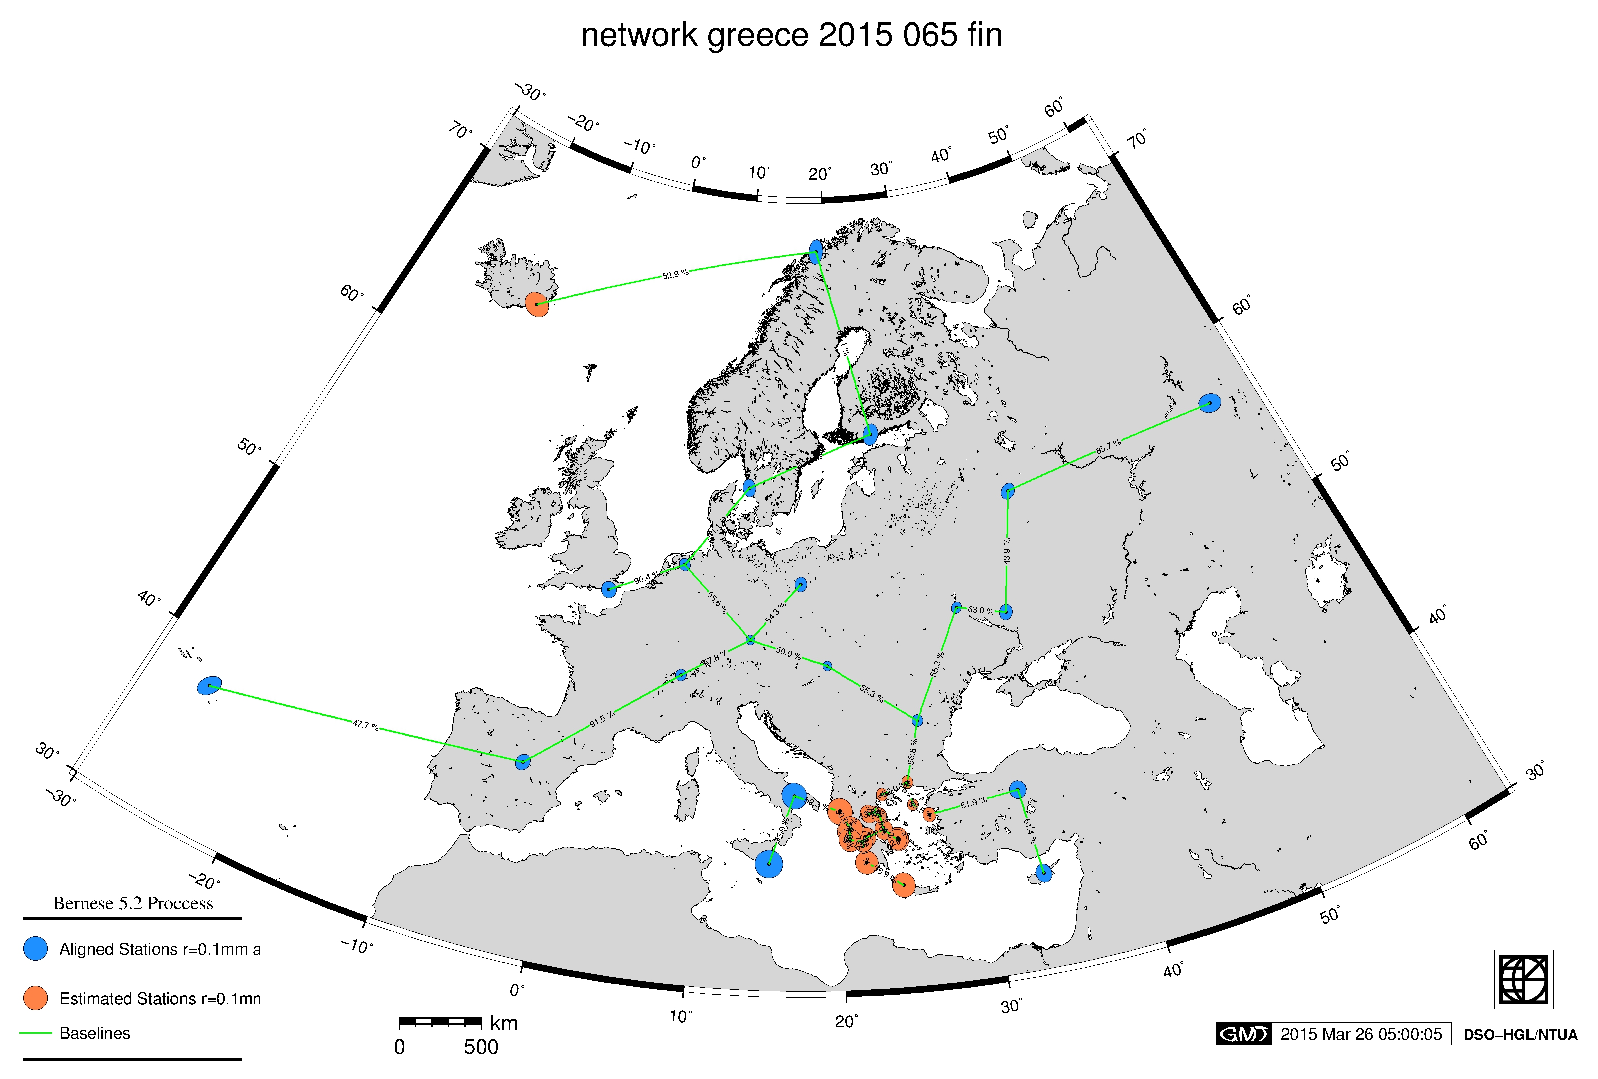
\includegraphics[trim={.2cm 1cm .2cm 0cm},clip,width=1\textwidth]{img/eu-greece-15065-fin-proc.eps} %1 2.2 0 0
%  \vskip -.7cm
 \caption{Χάρτης με τις σχηματισμένες βάσης για την υλοποίηση του συστήματος αναφοράς}
 \label{fig:igsbl}
 \end{center}
 \end{figure}


\end{column}
\end{columns}

\end{frame}


\section{Αποτελέσματα}

\begin{frame}\frametitle{Τελικές συντεταγμένες σημείων Παναγοπούλας}\framesubtitle{}

\begin{table}[]
\caption{Τελικές συντεταγμένες - 1η Περίοδος μετρήσεων 15/2/2014}
\label{tab:plcrd01}
\vskip -.3cm
\centering
\resizebox{\textwidth}{!}{%
\begin{tabular}{{l} | *{2}{c} | *{2}{c} | *{2}{c}}
Κωδικός  & Χ (m) & σX(m) & Y(m) & σY(m) & Z(m) & σz(m) \\
\hline \hline
N000   & 4647168.058 & 0.00199 & 1871835.499 & 0.00091 & 3934052.529 & 0.00162 \\
PL01   & 4647391.899 & 0.00045 & 1871420.637 & 0.00022 & 3933993.484 & 0.00039 \\
PL02   & 4647365.954 & 0.00036 & 1871498.689 & 0.00021 & 3933985.844 & 0.00033 \\
PL03   & 4647480.571 & 0.00036 & 1871635.917 & 0.00020 & 3933922.995 & 0.00030 \\
PL04   & 4647309.908 & 0.00049 & 1871777.071 & 0.00028 & 3933949.500 & 0.00041 \\
PL05   & 4647325.668 & 0.00048 & 1871697.297 & 0.00028 & 3933962.207 & 0.00040 \\
PL06   & 4647315.748 & 0.00051 & 1871588.118 & 0.00028 & 3933998.231 & 0.00055 \\
\hline
\end{tabular}
}
\end{table}

\begin{table}[]
\caption{Τελικές Συντεταγμένες - 2η Περίοδος μετρήσεων 28/4/2015}
\label{tab:plcrd02}
\vskip -.3cm
\centering
\resizebox{\textwidth}{!}{%
\begin{tabular}{{l} | *{2}{c} | *{2}{c} | *{2}{c}}
Κωδικός  & Χ (m) & σX(m) & Y(m) & σY(m) & Z(m) & σz(m) \\
\hline \hline
N000     & 4647168.038 & 0.00248 & 1871835.506 & 0.00095 & 3934052.507 & 0.00192 \\
PL01     & 4647391.885 & 0.00056 & 1871420.640 & 0.00030 & 3933993.485 & 0.00065 \\
PL02     & 4647365.930 & 0.00062 & 1871498.695 & 0.00033 & 3933985.828 & 0.00072 \\
PL03     & 4647480.548 & 0.00049 & 1871635.924 & 0.00030 & 3933922.974 & 0.00045 \\
PL04     & 4647309.883 & 0.00054 & 1871777.076 & 0.00033 & 3933949.482 & 0.00058 \\
PL05     & 4647325.637 & 0.00141 & 1871697.308 & 0.00077 & 3933962.196 & 0.00122 \\
PL06     & 4647315.760 & 0.00134 & 1871588.108 & 0.00083 & 3933998.236 & 0.00087 \\
\hline
\end{tabular}
}
\end{table}

\end{frame}

\begin{frame}\frametitle{Τελικές συντεταγμένες σημείων Πλατάνου}\framesubtitle{}
\begin{table}[]
\caption{Τελικές συντεταγμένες - 1η Περίοδος μετρήσεων 16/2/2014}
\label{tab:plobs01}
\vskip -.5cm
\centering
\resizebox{\textwidth}{!}{%
\begin{tabular}{{l} | *{2}{c} | *{2}{c} | *{2}{c}}
Κωδικός  & Χ (m) & σX(m) & Y(m) & σY(m) & Z(m) & σz(m) \\
\hline \hline
PT01     & 4646574.450 & 0.00065 & 1902146.348 & 0.00041 & 3920386.261 & 0.00054 \\
PT02     & 4646625.032 & 0.00061 & 1902172.847 & 0.00041 & 3920341.291 & 0.00053 \\
PT03     & 4646576.114 & 0.00058 & 1902256.857 & 0.00044 & 3920351.762 & 0.00043 \\
PT04     & 4646505.053 & 0.00049 & 1902307.027 & 0.00031 & 3920373.754 & 0.00041 \\
PT05     & 4646514.457 & 0.00072 & 1902167.038 & 0.00035 & 3920424.469 & 0.00050 \\
PT06     & 4646518.166 & 0.00148 & 1902132.136 & 0.00061 & 3920439.943 & 0.00091 \\
PT07     & 4646123.606 & 0.00261 & 1902899.415 & 0.00118 & 3920455.035 & 0.00205 \\
PT08     & 4646450.016 & 0.00052 & 1902181.042 & 0.00035 & 3920470.901 & 0.00049 \\
\hline
\end{tabular}
}
\end{table}
\vskip -.2cm
\begin{table}[]
\caption{Τελικές Συντεταγμένες - 2η Περίοδος μετρήσεων 29/4/2015}
\label{tab:crd02}
\vskip -.5cm
\centering
\resizebox{\textwidth}{!}{%
\begin{tabular}{{l} | *{2}{c} | *{2}{c} | *{2}{c}}
Κωδικός  & Χ (m) & σX(m) & Y(m) & σY(m) & Z(m) & σz(m) \\
\hline \hline
PT01     & 4646574.458 & 0.00073 & 1902146.358 & 0.00048 & 3920386.270 & 0.00078 \\
PT02     & 4646625.032 & 0.00061 & 1902172.857 & 0.00043 & 3920341.301 & 0.00067 \\
PT03     & 4646576.101 & 0.00105 & 1902256.845 & 0.00070 & 3920351.767 & 0.00089 \\
PT04     & 4646505.076 & 0.00085 & 1902307.035 & 0.00048 & 3920373.761 & 0.00071 \\
PT05     & 4646514.465 & 0.00071 & 1902167.056 & 0.00048 & 3920424.478 & 0.00083 \\
PT06     & 4646518.165 & 0.00094 & 1902132.147 & 0.00057 & 3920439.945 & 0.00104 \\
PT07     & 4646123.615 & 0.00131 & 1902899.434 & 0.00056 & 3920455.046 & 0.00112 \\
PT08     & 4646450.043 & 0.00108 & 1902181.055 & 0.00057 & 3920470.903 & 0.00047 \\
\hline
\end{tabular}
}
\end{table}

\end{frame}


\begin{frame}\frametitle{Μετατοπίσεις στην περιοχή της Παναγοπούλας}\framesubtitle{}
\begin{columns}[T] % align columns
\begin{column}{.3\textwidth}

\begin{table}[]
\caption{Διαφορές συντεταγμένων - Παναγοπούλα}
\label{tab:pldisp}
% \vskip -.5cm
\centering
\resizebox{\textwidth}{!}{%
\begin{tabular}{{l} | *{3}{c}}
Κωδικός  & dN (m) & dE (m) & dU (m) \\
\hline \hline
N000  & -0.007 & 0.014 & -0.026 \\
PL01  & 0.009 & 0.008 & -0.009 \\
PL02 & 0.000 & 0.015 & -0.025 \\
PL03 & -0.004 & 0.015 & -0.028 \\
PL04 & -0.001 & 0.014 & -0.027 \\
PL05 & 0.007 & 0.021 & -0.026 \\
PL06 & 0.000 & -0.014 & 0.009 \\
\hline
\end{tabular}
}
\end{table}

\end{column}

\begin{column}{.7\textwidth}
\begin{figure}
 \begin{center}
 \vskip -.5cm
 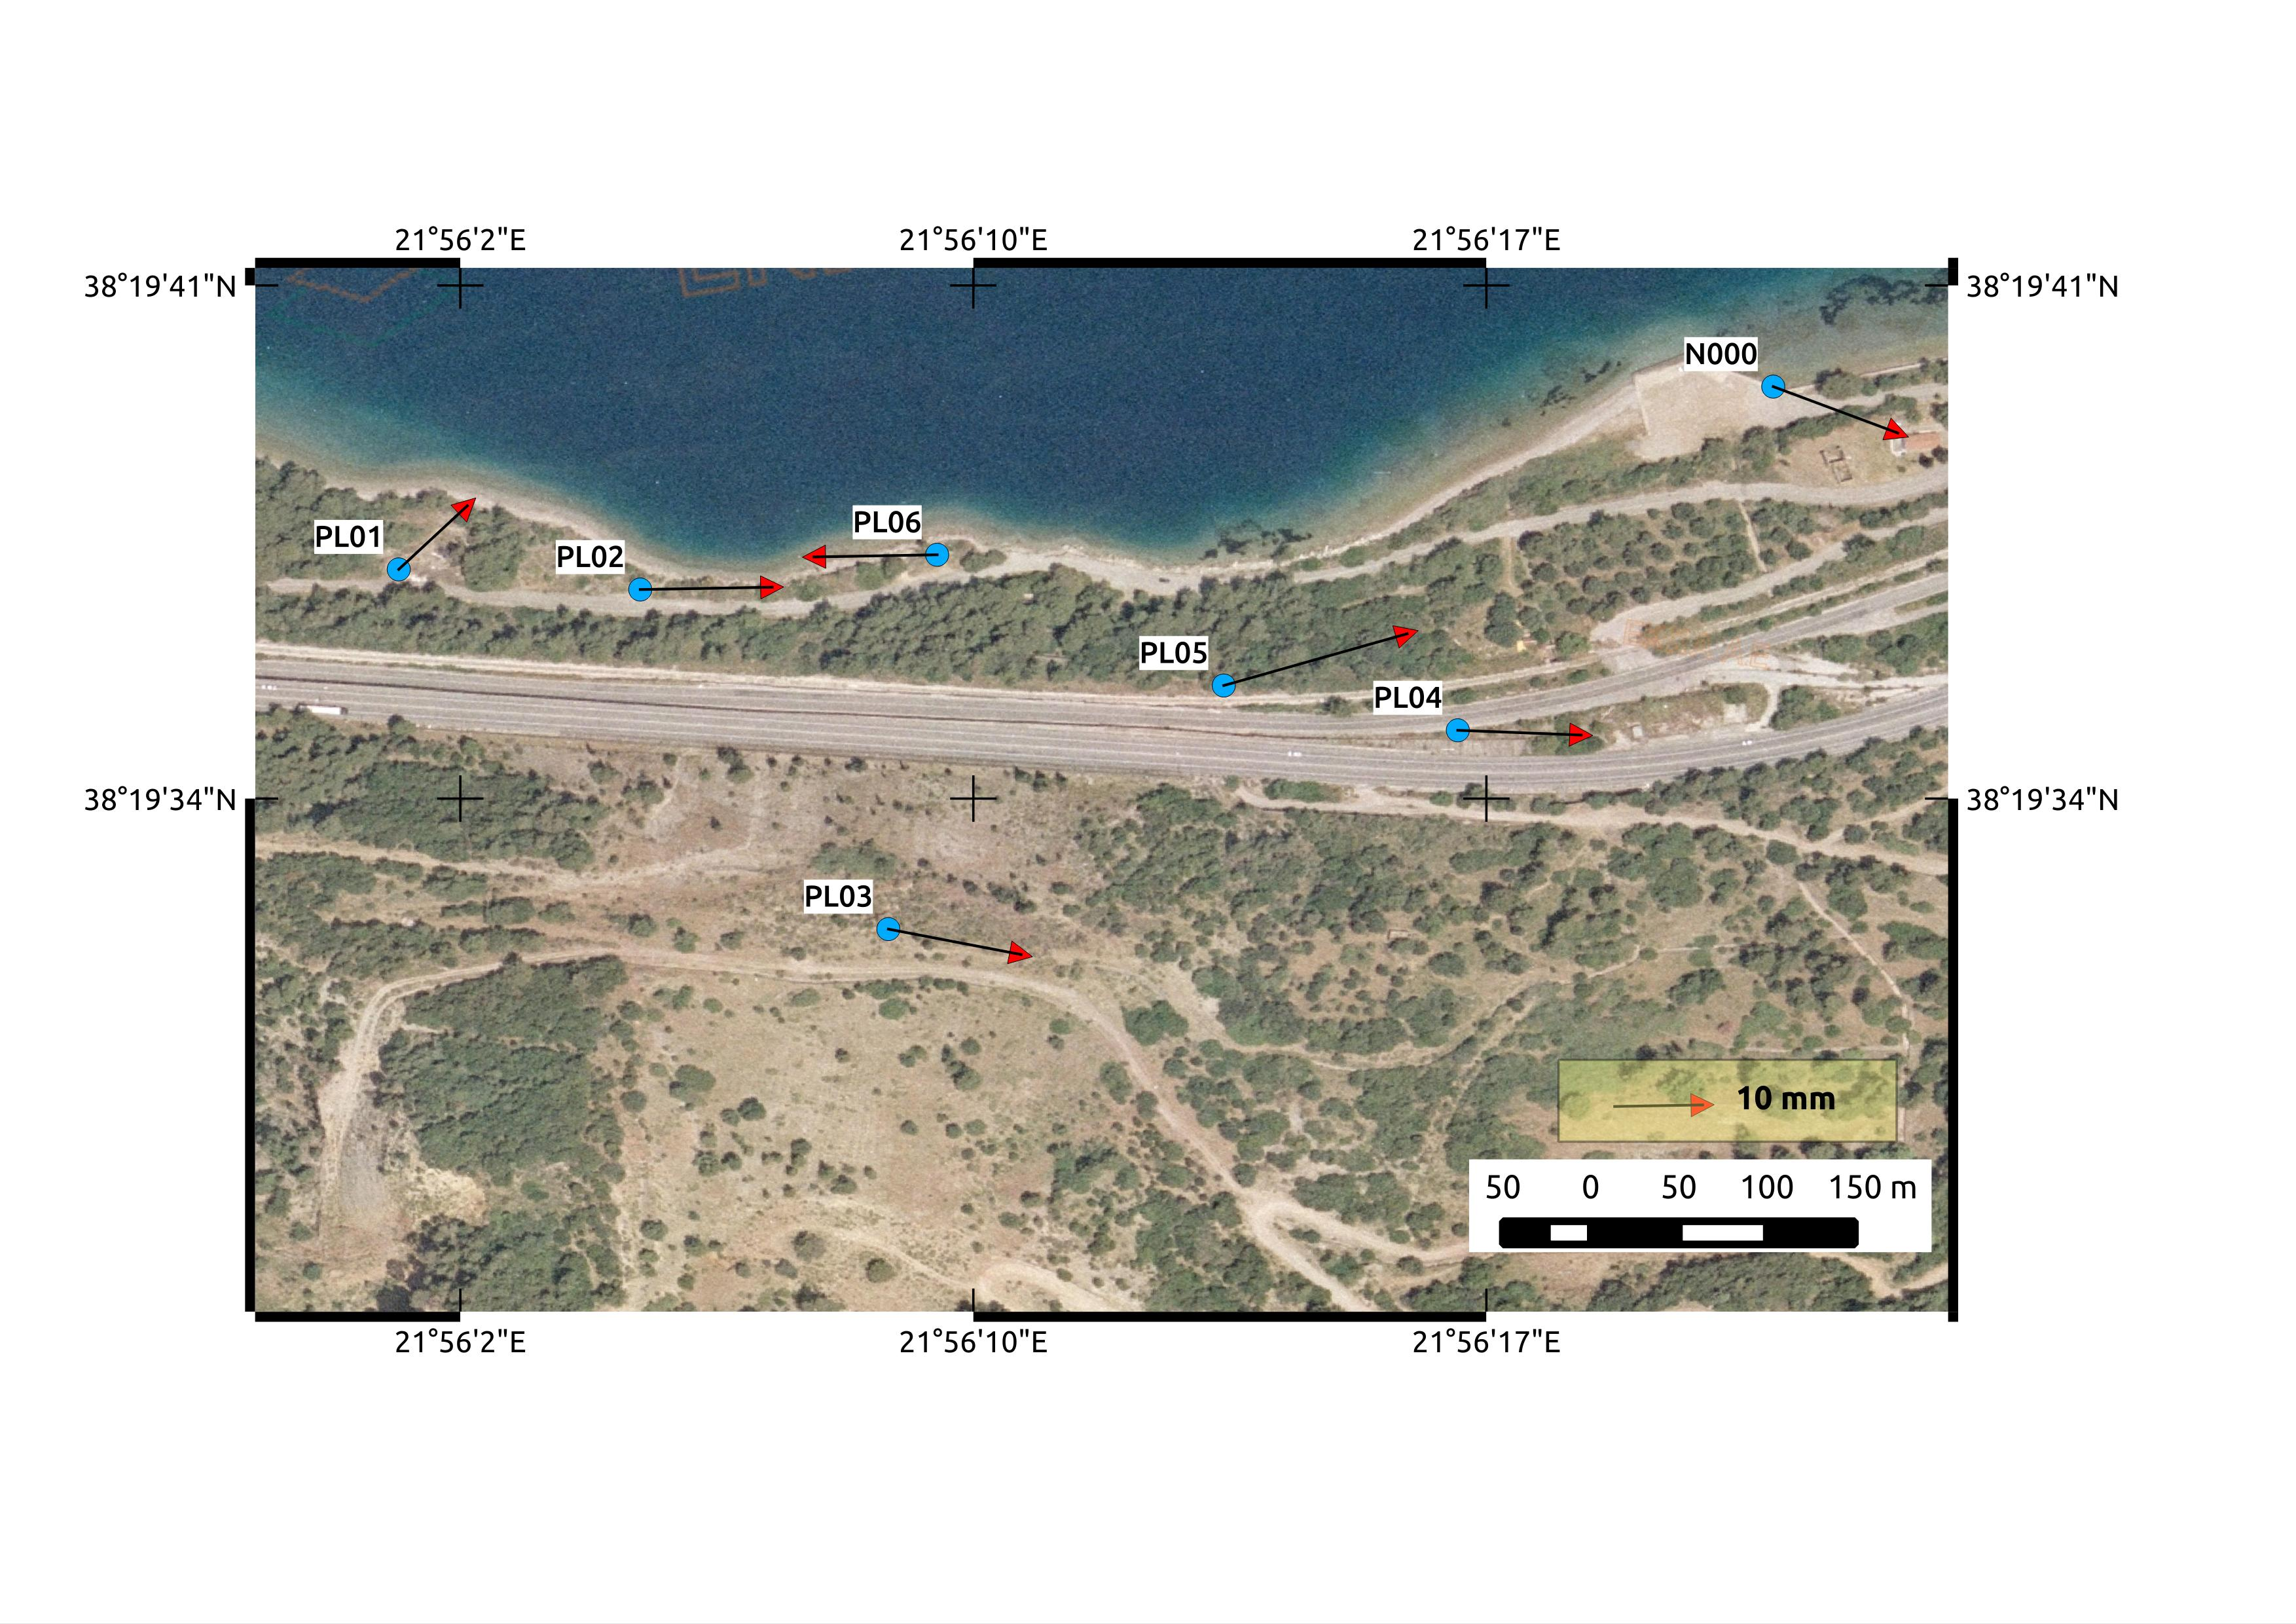
\includegraphics[trim={1cm 2.5cm 1cm 2cm},clip,width=1.1\textwidth]{img/panagopoula-disp.jpg} %1 2.2 0 0
%  \vskip -.7cm
 \caption{Διαφορές συντεταγμένων στην περιοχή της Παναγοπούλας}
 \label{fig:pldisp}
 \end{center}
 \end{figure}


\end{column}
\end{columns}
\end{frame}

\begin{frame}\frametitle{Μετατοπίσεις στην περιοχή του Πλατάνου}\framesubtitle{}
\begin{columns}[T] % align columns
\begin{column}{.3\textwidth}

\begin{table}[]
\caption{Διαφορές συντεταγμένων - Πλάτανος}
\label{tab:ptdisp}
% \vskip -.5cm
\centering
\resizebox{\textwidth}{!}{%
\begin{tabular}{{l} | *{3}{c}}
Κωδικός  & dN (m) & dE (m) & dU (m) \\
\hline \hline
PT01  & -0.001 & 0.007 & 0.014 \\
PT02  & 0.005 & 0.009 & 0.009 \\
PT03  & 0.016 & -0.006 & -0.008 \\
PT04  & -0.010 & -0.001 & 0.023 \\
PT05  & -0.002 & 0.013 & 0.017 \\
PT06  & -0.001 & 0.010 & 0.004 \\
PT07  & -0.001 & 0.014 & 0.019 \\
PT08  & -0.017 & 0.002 & 0.025 \\
\hline
\end{tabular}
}
\end{table}

\end{column}

\begin{column}{.7\textwidth}
\begin{figure}
 \begin{center}
 \vskip -.5cm
 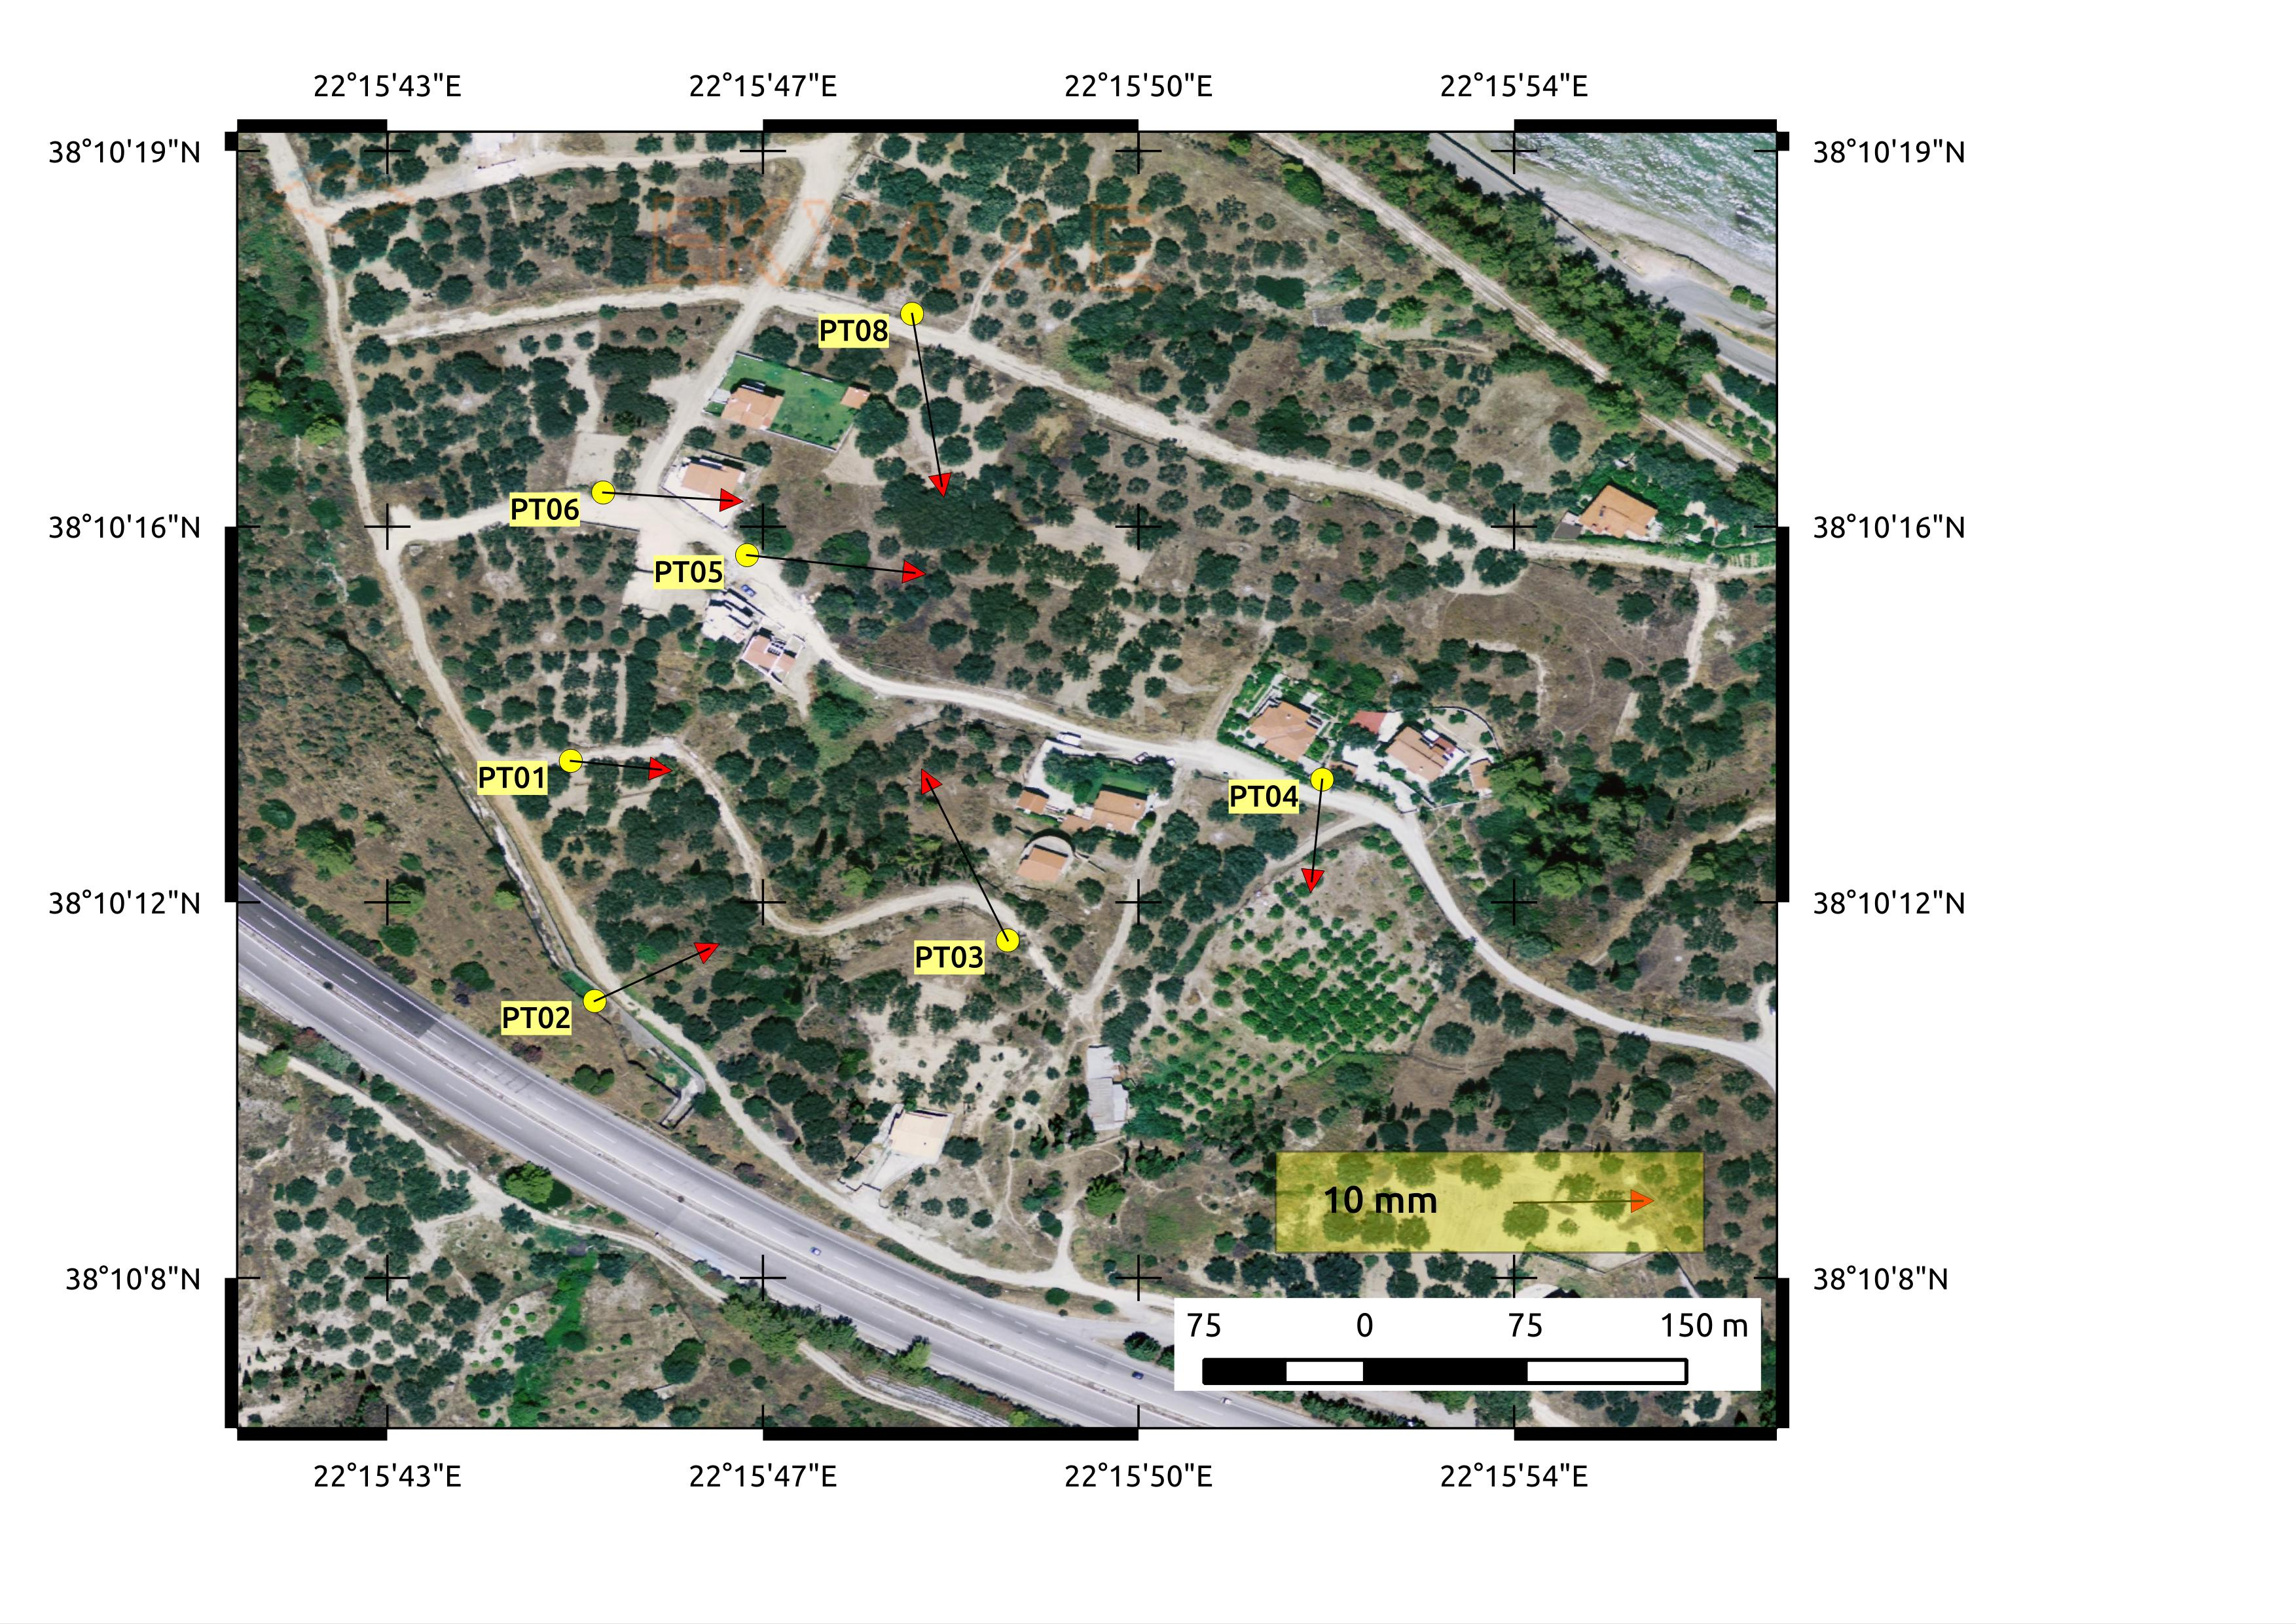
\includegraphics[trim={1cm 2.5cm 2.5cm .5cm},clip,width=1.1\textwidth]{img/platanos-disp.jpg} %1 2.2 0 0
%  \vskip -.7cm
 \caption{Διαφορές συντεταγμένων στην περιοχή του Πλατάνου}
 \label{fig:ptdisp}
 \end{center}
 \end{figure}


\end{column}
\end{columns}
\end{frame}

\begin{frame}\frametitle{......}\framesubtitle{}
\textcolor{red}{να γράψουμε κανα κονκλουσιον??}
\end{frame}


% \section{GPS/GNSS Networks in Greece}
% 
% \begin{frame}\frametitle{Densification Network Selection}\framesubtitle{}
%   To contribute to the Densification we have to establish a credible dataset
%   (network). This has proven to be rather challenging !\\
%   \bigskip
%   Currently we process whatever we can get our hands on \ldots\\
%   Problems:
%   \begin{itemize}
%     \item Inhomogenous dataset (\texttt{RINEX}, raw files, etc).
%     \item Various maintainers, different mentalities.
%     \item Different aquisition methods/rates.
%     \item Hardly any log files.
%     \item Wide variety of equipment (not always included in \texttt{atx} files).
%   \end{itemize}
% \end{frame}
% 
% \begin{frame}\frametitle{COMET/NTUA Network}\framesubtitle{}
% %Network installed/maintained by \texttt{COMET}\footnote{Center for Observation and Modeling of Earthquakes, \url{http://comet.nerc.ac.uk/}} \& \texttt{NTUA}.
% \begin{columns}[T] % align columns
% \begin{column}{.40\textwidth}
%   {\small
%   \begin{itemize}
%     \setlength\itemsep{.1em}
%     \item<pro@1-> established along the Hellenic Arc
%     \item<pro@1-> homogenous (geodetic type) equipment
%     \item<pro@1-> credible time-span (early 2004 - late 2011)
%     \item<con@1-> data aquisition stoped at late 2011
%     \item<con@1-> equipment is old \& GPS-only
%     \item<con@1-> needs repairing
% \end{itemize}
% }
% \end{column}%
% \hfill%
% \begin{column}{.60\textwidth}
%  \begin{figure}
%  \begin{center}
%  \vskip -.2cm
%  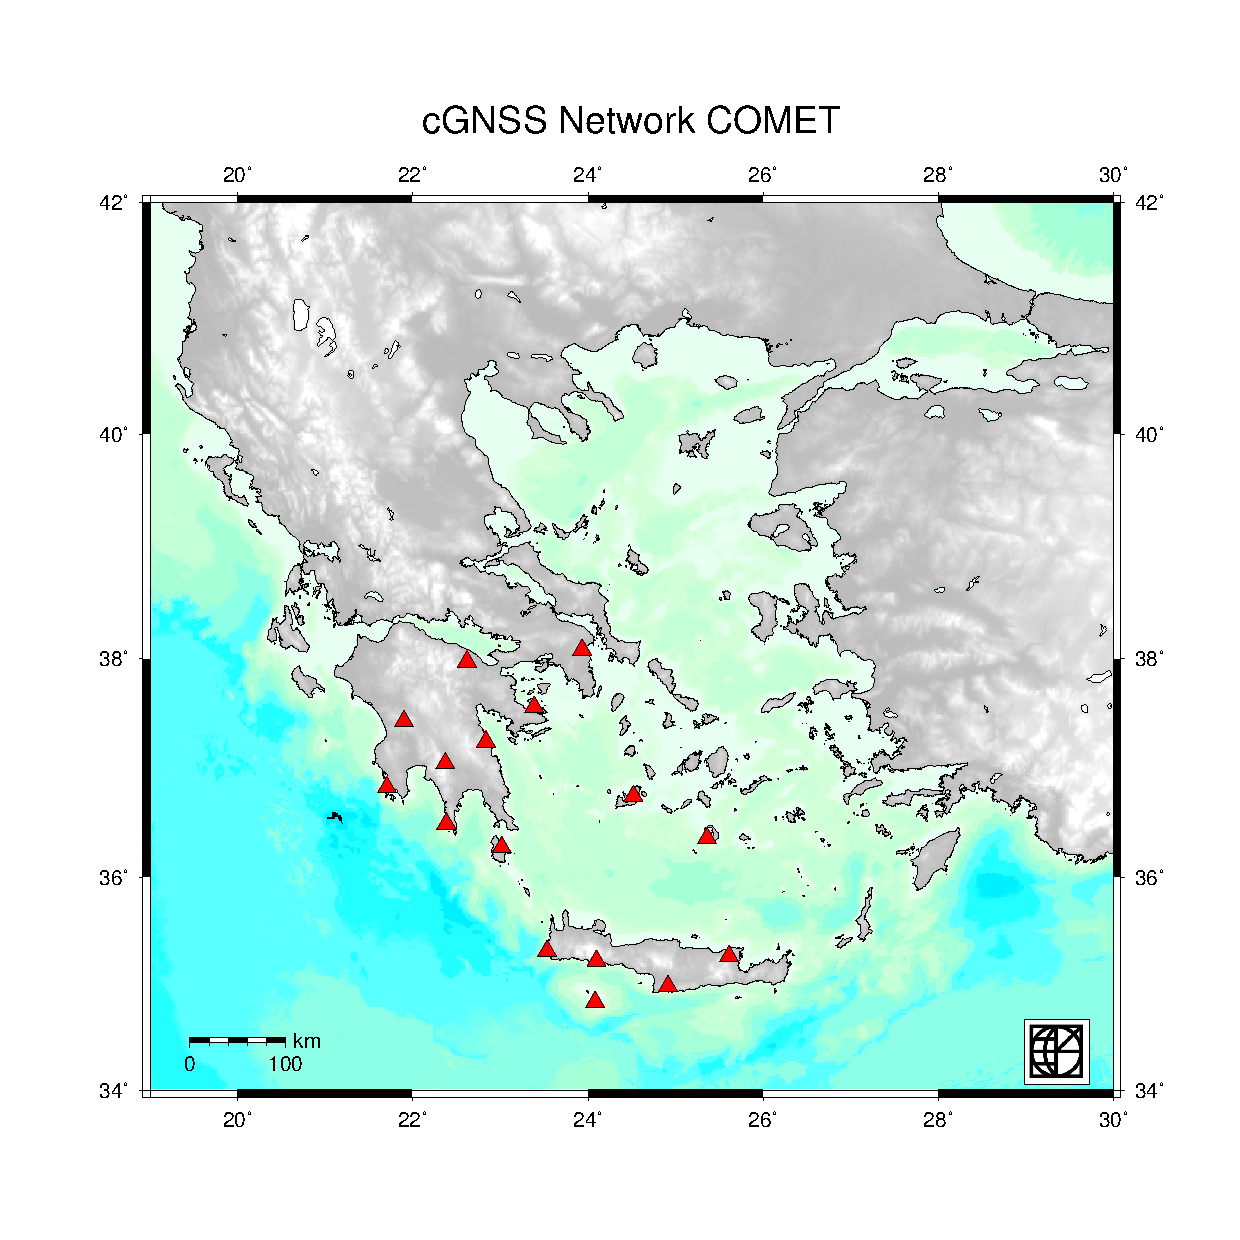
\includegraphics[trim={0cm 2.5cm 0cm 0cm},clip,width=.95\textwidth]{img/comet.eps} %1 2.2 0 0
%  \vskip -.7cm
%  \caption{COMET/NTUA network.}
%  \label{fig:cometntua}
%  \end{center}
%  \end{figure}
% \end{column}%
% \end{columns}
%   \begin{block}{}
%     Can be used for EUREF densification ``as is''.
%   \end{block}
% \end{frame}
% 
% \begin{frame}\frametitle{NOA/GEIN and others}\framesubtitle{}
% %Network maintained by \texttt{GEIN}/\texttt{NOA}\footnote{National Observatory of Athens \url{http://www.gein.noa.gr/services/GPS/noa\_gps.html}}. Sites established by various institutes
% %(\texttt{NTUA, UNAVCO, MIT}).
% \begin{columns}[T] % align columns
% \begin{column}{.40\textwidth}
%   \begin{itemize}
%     \item<pro@1-> covers (sparsely) all of Greece 
%     \item<pro@1-> credible time-span (newest stations at 2012)
%     \item<con@1-> inconsistent providers (for some stations)
%     \item<con@1-> no log files
%   \end{itemize}
% \end{column}%
% \hfill%
% \begin{column}{.60\textwidth}
%  \begin{figure}
%  \begin{center}
%  \vskip -.2cm
%  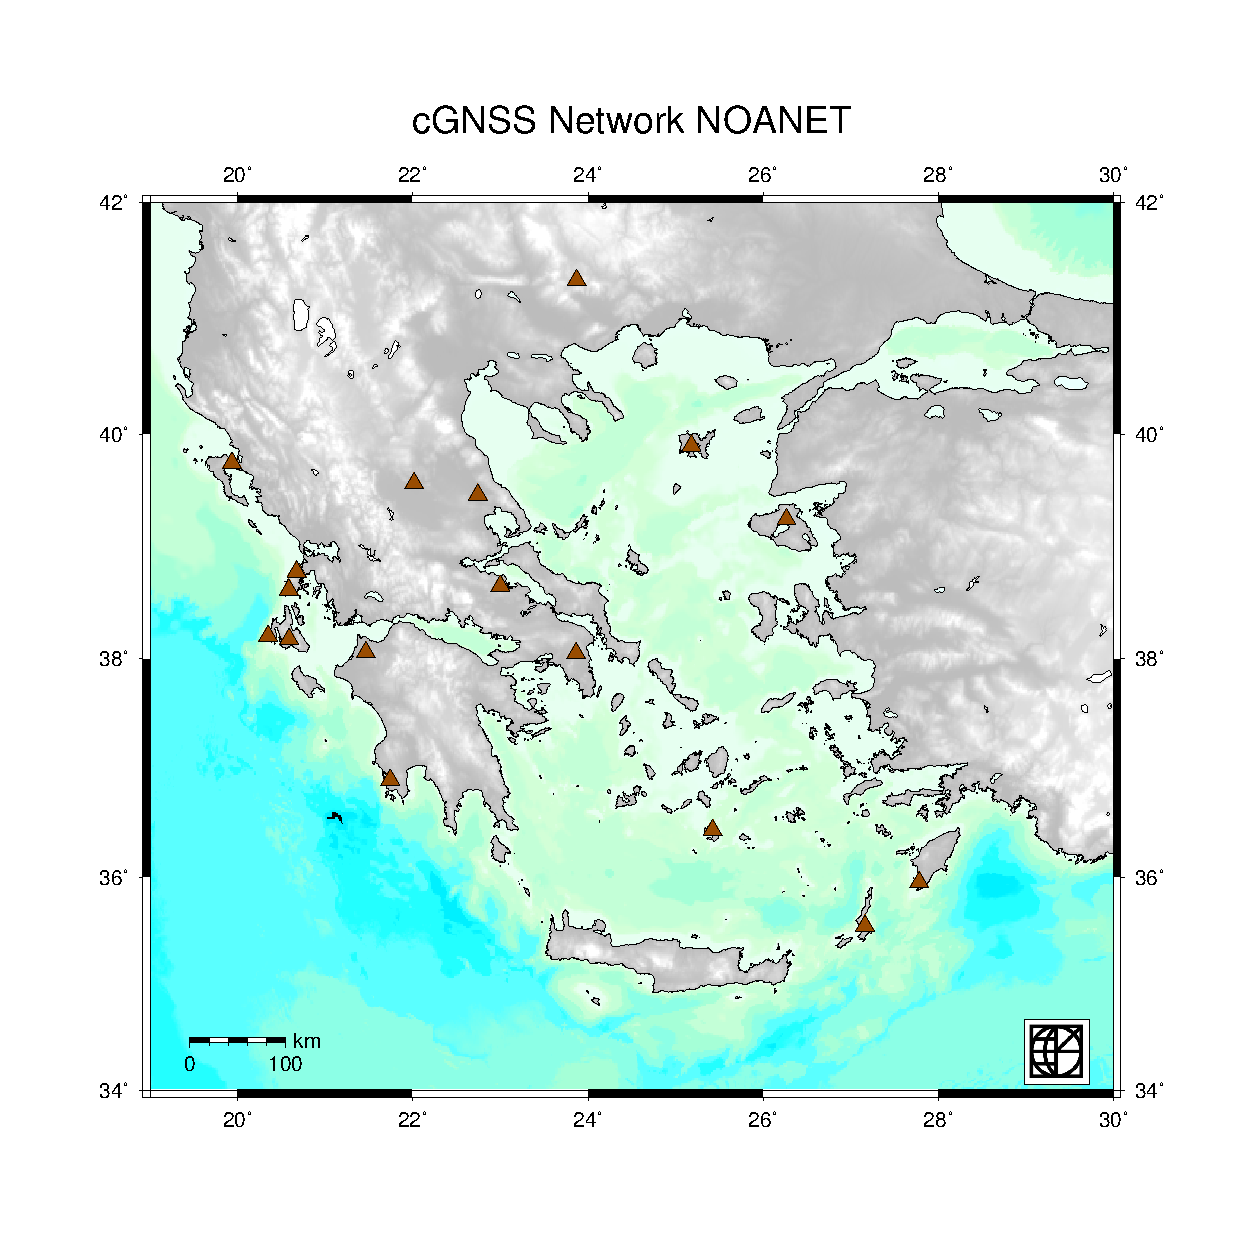
\includegraphics[trim={0cm 2.5cm 0cm 0cm},clip,width=.95\textwidth]{img/noanet.eps}
%  \vskip -.7cm
%  \caption{NOA/GEIN network.}
%  \label{fig:noa}
%  \end{center}
%  \end{figure}
% \end{column}%
% \end{columns}
%   \begin{block}{}
%     Unusable sites: atal, stef (no calibration).
%   \end{block}
% \end{frame}
% 
% \begin{frame}\frametitle{Tree-Company / URANUS}\framesubtitle{}
% %  Network installed/maintained by \texttt{Tree-Company}\footnote{URANUS network \url{http://www.uranus.gr/}}.
% \begin{columns}[T] % align columns
% \begin{column}{.35\textwidth}
% {\small
%   \begin{itemize}
%     \item<pro@1-> dense network, covers all of Greece
%     \item<pro@1-> homogenous (geodetic type) equipment
%     \item<con@1-> limited time-span (late 2013 onwards)
%     \item<con@1-> no log files
%     \item<con@1-> comercial usage oriented
%     \item<con@1-> $\sim$ 2 years of data lost !
%   \end{itemize}
%   }
% \end{column}%
% \hfill%
% \begin{column}{.65\textwidth}
%  \begin{figure}
%  \begin{center}
%  \vskip .5cm
%  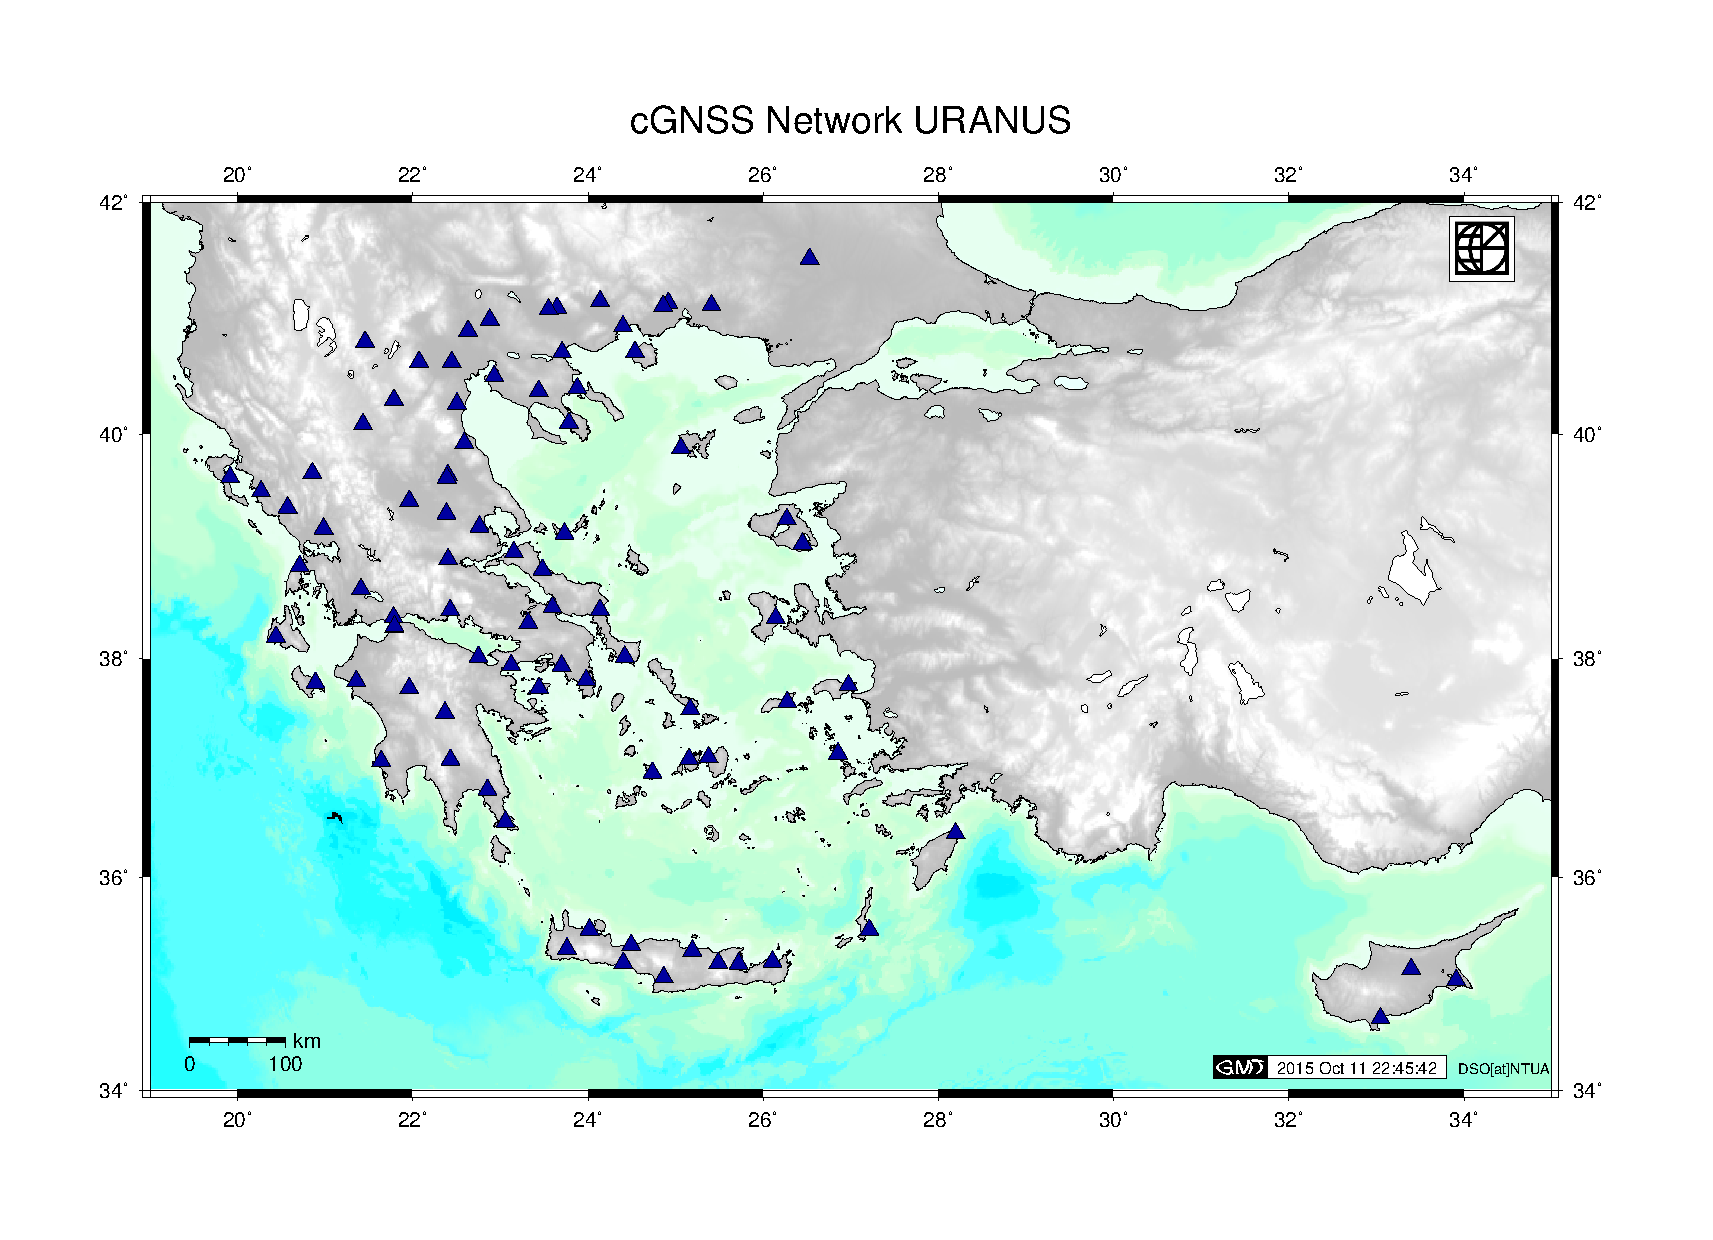
\includegraphics[trim={0cm 2.5cm 0cm 0cm},clip,width=1.1\textwidth]{img/uranus.eps}
%  \vskip -.4cm
%  \caption{Tree-Company URANUS network.}
%  \label{fig:uranus}
%  \end{center}
%  \end{figure}
% \end{column}%
% \end{columns}
%   \begin{block}{}
%   Can only use sites with time-span > 2 years. 
%   \end{block}
% \end{frame}
% 
% \begin{frame}\frametitle{HEPOS}\framesubtitle{}
% %  Network installed/maintained by \texttt{HEPOS}\footnote{\url{http://www.hepos.gr/}} (Greek Cadastre Service). 
% \begin{columns}[T] % align columns
% \begin{column}{.40\textwidth}
%   \begin{itemize}
%     \item<pro@1-> dense network, covers all of Greece
%     \item<pro@1-> homogenous (geodetic type) equipment
%     \item<con@1-> credible time-span (late 2007 onwards)
%     \item<con@1-> limited access ($\sim$5 stations)!!
%   \end{itemize}
% \end{column}%
% \hfill%
% \begin{column}{.68\textwidth}
%  \begin{figure}
%  \begin{center}
%  \vskip -.2cm
%  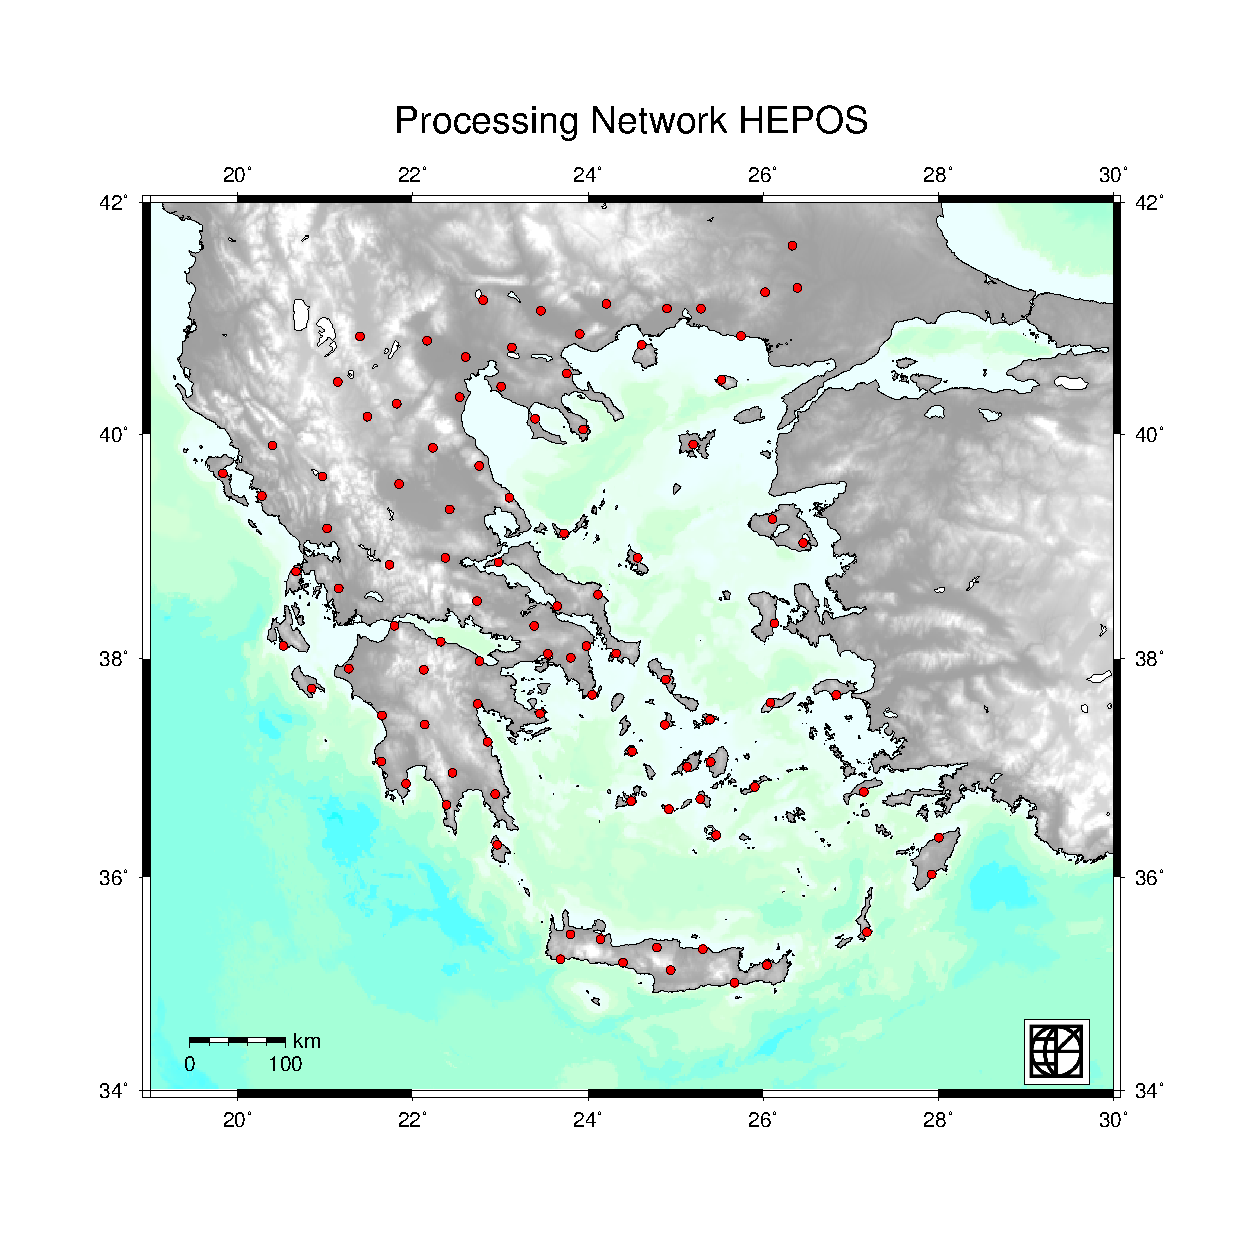
\includegraphics[trim={0cm 2.5cm 0cm 0cm},clip,width=.95\textwidth]{img/heposnet.eps}
%  \vskip -.7cm
%  \caption{HEPOS network.}
%  \label{fig:hepos}
%  \end{center}
%  \end{figure}
% \end{column}%
% \end{columns}
%   \begin{block}{}
%   Can only use somewhere between 5 and 10 sites for a time-span of $\sim$ 4 years.
%   \end{block}
% \end{frame}
% 
% \begin{frame}\frametitle{Local Networks}\framesubtitle{}
%   %Network installed/maintained by \texttt{CRLab}\footnote{Rift Laboratory \url{http://webobs.crlab.eu/}}. 
%   \FourQuad
%   {
%   \textbf{Corinth Rift.}
%   \begin{itemize}
%     \item<pro@1-> credible time-span
%     \item<pro@1-> only covers the Corinth Rift
%     \item<con@1-> inconsistent providers
%     \item<con@1-> no log files \& equipment changes
%   \end{itemize}
%   }
%   {
%  \begin{figure}
%  \begin{center}
%  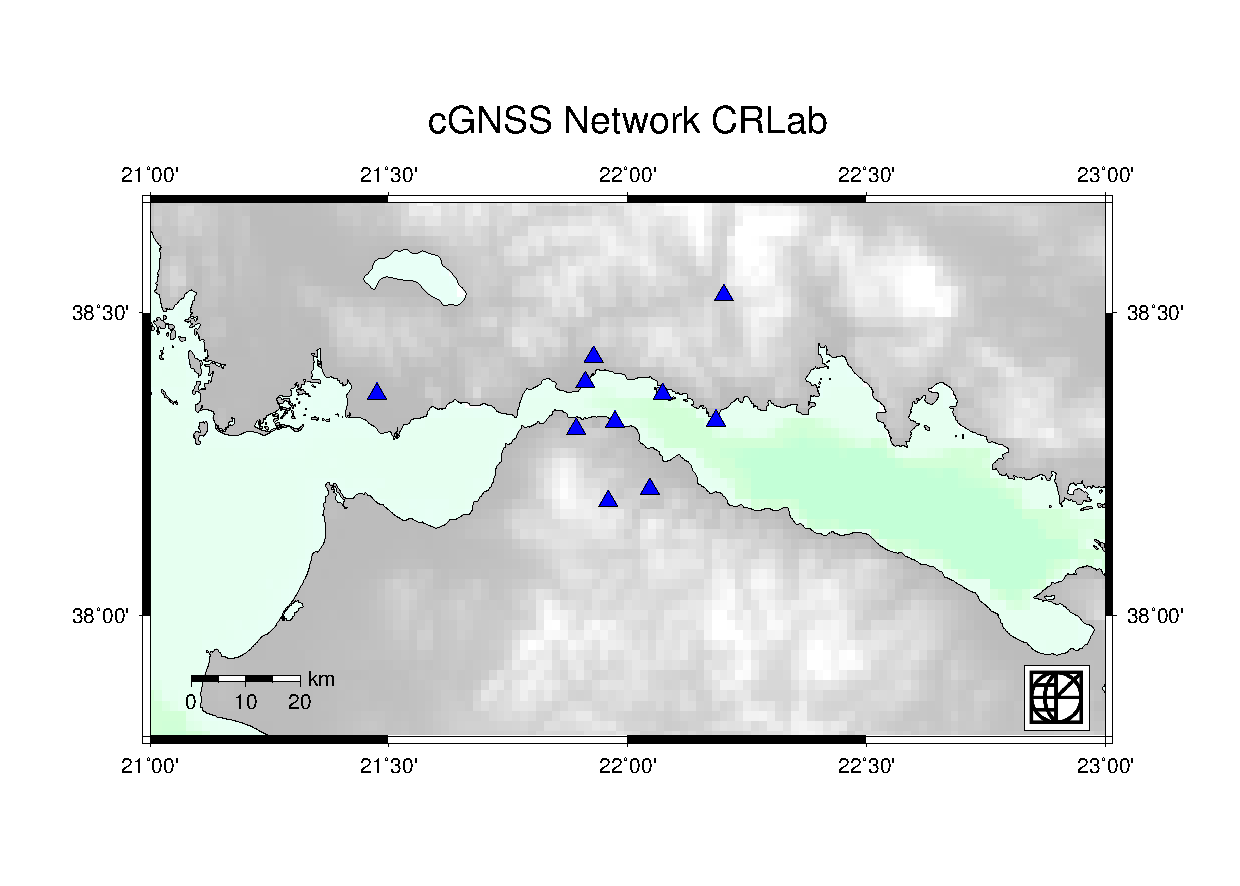
\includegraphics[trim={0cm 2.5cm 0cm 0cm},clip,width=.95\textwidth]{img/crlnet.eps}
%   \vskip -.6cm
%  \caption{CRLab network.}
%  \label{fig:crlab}
%  \end{center}
%  \end{figure}
%   }
%   {
%   \textbf{Santorini Network.}
%   Most of the stations installed post-2011 to monitor the \textit{inflation episode}.
%   \begin{itemize}
%     \item<con@1-> localized
%     \item<con@1-> limited time-span
%   \end{itemize}
%   }
%   {
%  \begin{figure}
%  \begin{center}
%  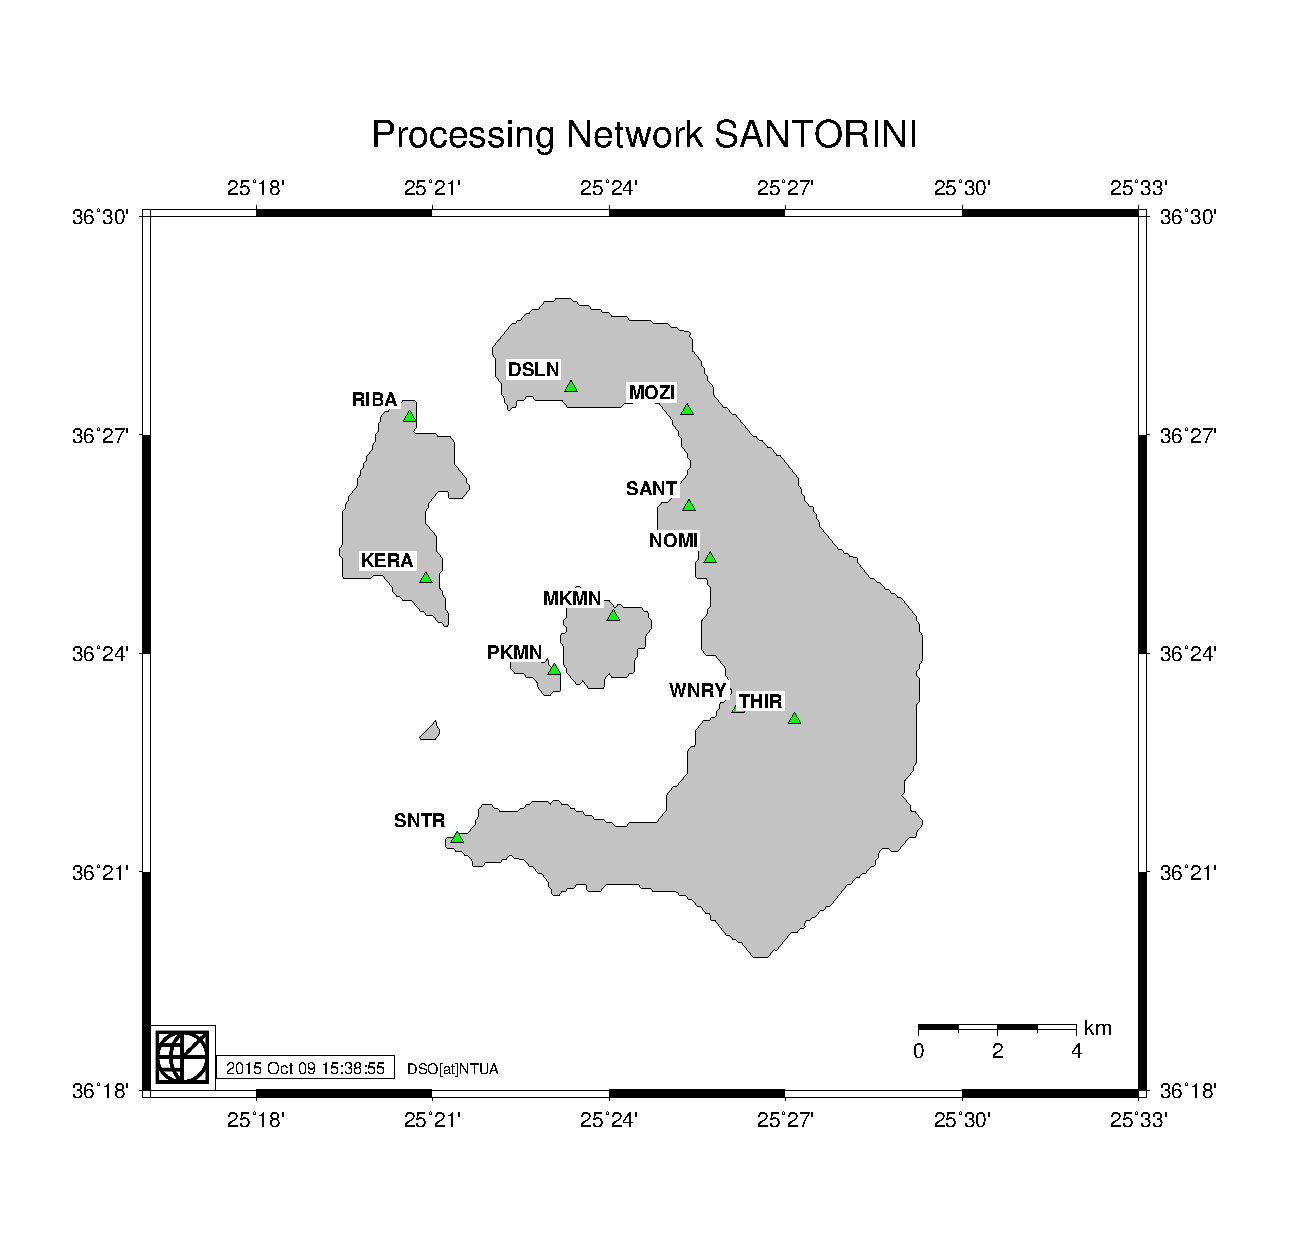
\includegraphics[trim={0cm 2.5cm 0cm 0cm},clip,width=.85\textwidth]{img/sntrnet.eps}
%   \vskip -.6cm
%  \caption{Santorini network.}
%  \label{fig:sntrnet}
%  \end{center}
%  \end{figure}
%   }
% \end{frame}
% 
% \begin{frame}\frametitle{Densification Network}\framesubtitle{}
%   The network to be used for the Densification, will look something like this \ldots
%  \begin{figure}
%  \begin{center}
%  \vskip -.2cm
%  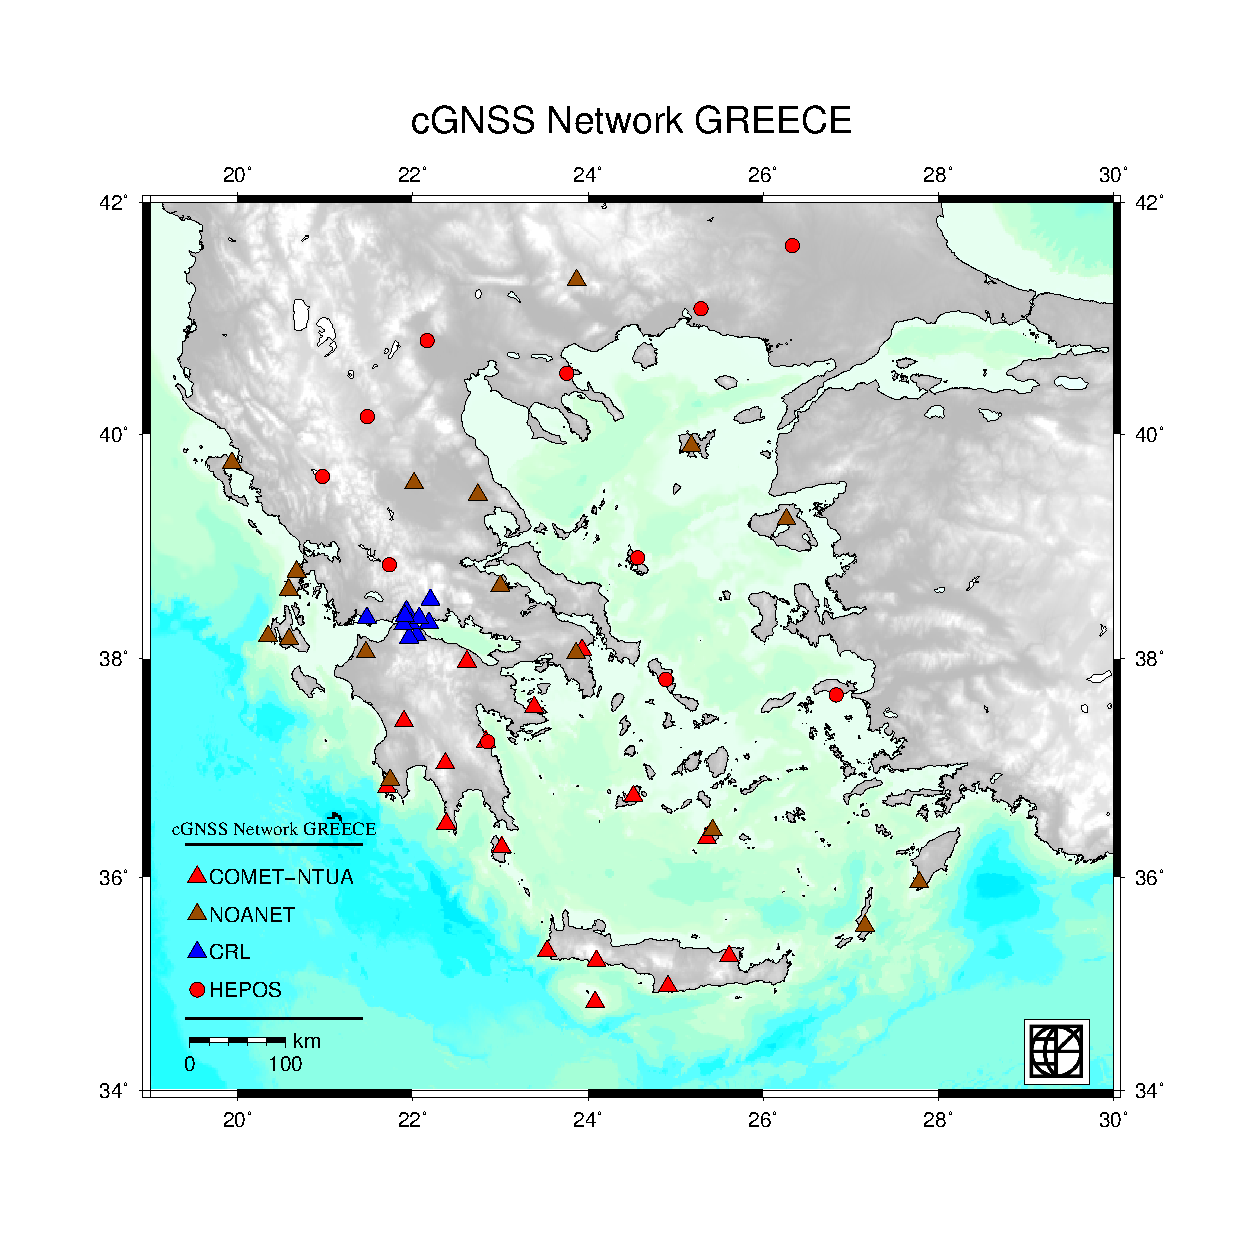
\includegraphics[trim={0cm 2.5cm 0cm 0cm},clip,width=.75\textwidth]{img/greeceall.eps}
%   \vskip -.7cm
%  \caption{Densification network (preliminary).}
%  \label{fig:dgrm}
%  \end{center}
%  \end{figure}
% \end{frame}
% 
% \section{Processing}
% 
% \begin{frame}\frametitle{The Scheme}\framesubtitle{}
% \begin{columns}[T] % align columns
% \begin{column}{.28\textwidth}
%   The core tool/software is \texttt{Bernese GNSS Software v5.2}\cite{bpe}.\\
%   \medskip
%   Integration with 
%   \begin{itemize}
%     \item \texttt{MySQL} database,
%     \item \texttt{Python} library
%     \item \texttt{GSAC}
%     \item wrappers (\texttt{shell})
%   \end{itemize}
% \end{column}%
% \hfill%
% \begin{column}{.68\textwidth}
% \vskip -1cm
% \begin{tikzpicture}[ every annotation/.style = {draw,
%                      fill = white, font = \large}]
% 
%   \path[mindmap,concept color=black!40,text=white,
%     every node/.style={concept,circular drop shadow, scale=.4},
%     root/.style = {concept color=black!40,
%       font=\normalsize\bfseries,text width=5em},
%     level 1 concept/.append style={font=\normalsize\bfseries,
%       sibling angle=50,text width=7.7em,
%     level distance=20mm,inner sep=0pt},
%     level 2 concept/.append style={font=\bfseries,level distance=15mm},
%   ]
% 
%   node[root] {Bernese GNSS Software v5.2} [clockwise from=0]
%     child[concept color=blue!60] {
%       node {bernutils Python library} [clockwise from=90]
%       child { node[concept] {github repo} }
%       child { node[concept] {modules for Bernese output/control files} }
%       child { node[concept] {modules for products} }
%     }
%     child[concept color=blue] {
%       node[concept] {MySQL Database} [clockwise from=0]
%       child { node[concept] {Bernese .STA} }
%       child { node[concept] {IGS log files} }
%       child { node[concept] {stations/networks/products} }
%     }
%     child[concept color=red] {
%       node[concept] {/bin wrappers \& utils } [clockwise from=270]
%       child { node[concept] {glue everything together} }
%       child { node[concept] {various utilities \& formating} }
%     }
%     child[concept color=yellow!60!black] {
%       node[concept] { GSAC } [clockwise from=220]
%       child { node[concept] {RINEX} }
%       child { node[concept] {products} }
%     }
%     child[concept color=green!40!black] {
%       node[concept] { WebPage } [clockwise from=300]
%     }
%     \end{tikzpicture}
% \end{column}%
% \end{columns}
% \end{frame}
% 
% \begin{frame}\frametitle{Compliance wrt EUREF standards}\framesubtitle{}
%   Processing is consistent with EUREFF standards (\href{http://www.epncb.oma.be/_documentation/guidelines/guidelines_analysis_centres.pdf}{Guidelines for Analysis Centres}).
%   \begin{itemize}%%[label={\checkmark}]
%     \item \texttt{SINEX} with required info/blocks,
%     \item Reference frame \texttt{IGb08},
%     \item \texttt{IERS} Conventions 2010,
%     \item \texttt{IGS}/\texttt{CODE} products,
%     \item ocean loading corrections (\texttt{FES2004}),
%     \item atmospheric tidal loading corrections,
%     \item $3^{\circ}$ elevation cut-off angle; elevation dependent weighting,
%     \item \texttt{GMF} and/or \texttt{VMF1}; \texttt{Chen-Herring} gradient parameter,
%     \item amiguities fixed (length-dependent algorithm),
%     \item use \texttt{GLONASS} obs (when available)
%   \end{itemize}
% \end{frame}
% 
% %  \begin{itemize}
% %    \item check station information file consistency (against the provided in \texttt{CODE}'s ftp)
% %    \item synchronize \texttt{GEN/} directory
% %    \item closely follow \texttt{RNX2SNX.PCF}
% %    \begin{itemize}
% %      \item variabes in PCF are set by external tools (genericity)
% %      \item skip copying/moving/removing; replace with tools that interconnect with \texttt{MySQL}
% %    \end{itemize}
% %    \item update database
% %    \item customize output (\texttt{html, json})
% %  \end{itemize}
% % \end{frame}
% 
% \begin{frame}\frametitle{Workflow}\framesubtitle{}
% \begin{columns}[T] % align columns
% \begin{column}{.48\textwidth}
%   \texttt{\$>ddproces.sh --year= --doy= --session= --bern-loadgps= --campaign= --satellite-system= --solution-id= --save-dir= --analysis-center= --use-ntua-products= --append-suffix= --elevation-angle= --update= --pcv= --apply-exclude-list}
% \end{column}
% \hfill%
% \begin{column}{.48\textwidth}
%   \scalebox{0.5}{
%   \smartdiagram[priority descriptive diagram]{
%     Download \texttt{RINEX} consulting \texttt{MySQL} db,
%     Download products,
%     Validate \texttt{.STA}; synchronize \texttt{/GEN},
%     Set variables in the Protocol Control File (\texttt{.PCF}),
%     Process the dataset,
%     Check for errors,
%     Save Products \& Update database records,
%     Compile Report (\texttt{json} | \texttt{html})
% }}
% \end{column}
% \end{columns}
% \end{frame}
% 
% {
% \usebackgroundtemplate{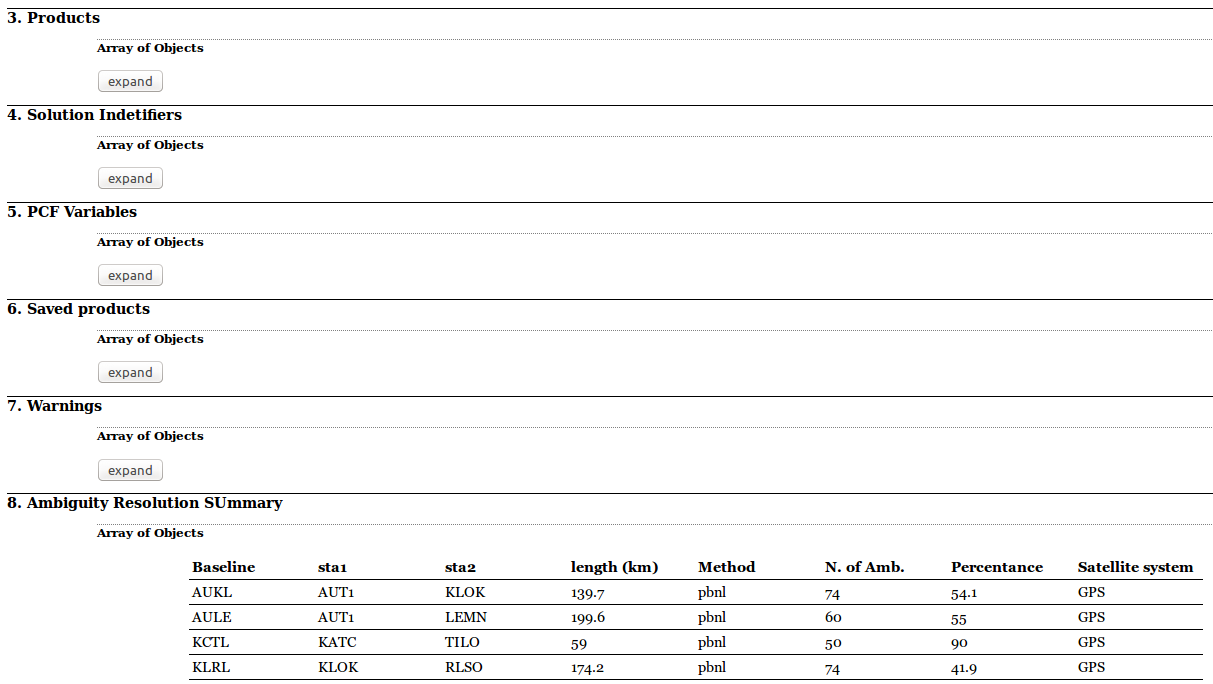
\includegraphics[height=.9\paperheight,width=.9\paperwidth]{img/jsonprint.png}}
% \begin{frame}\frametitle{Results \& Output}\framesubtitle{}
% \begin{center}
% \vskip -1.6cm
% \begin{tikzpicture}
%   \node (img1) {\shadowbox{\color{black!35}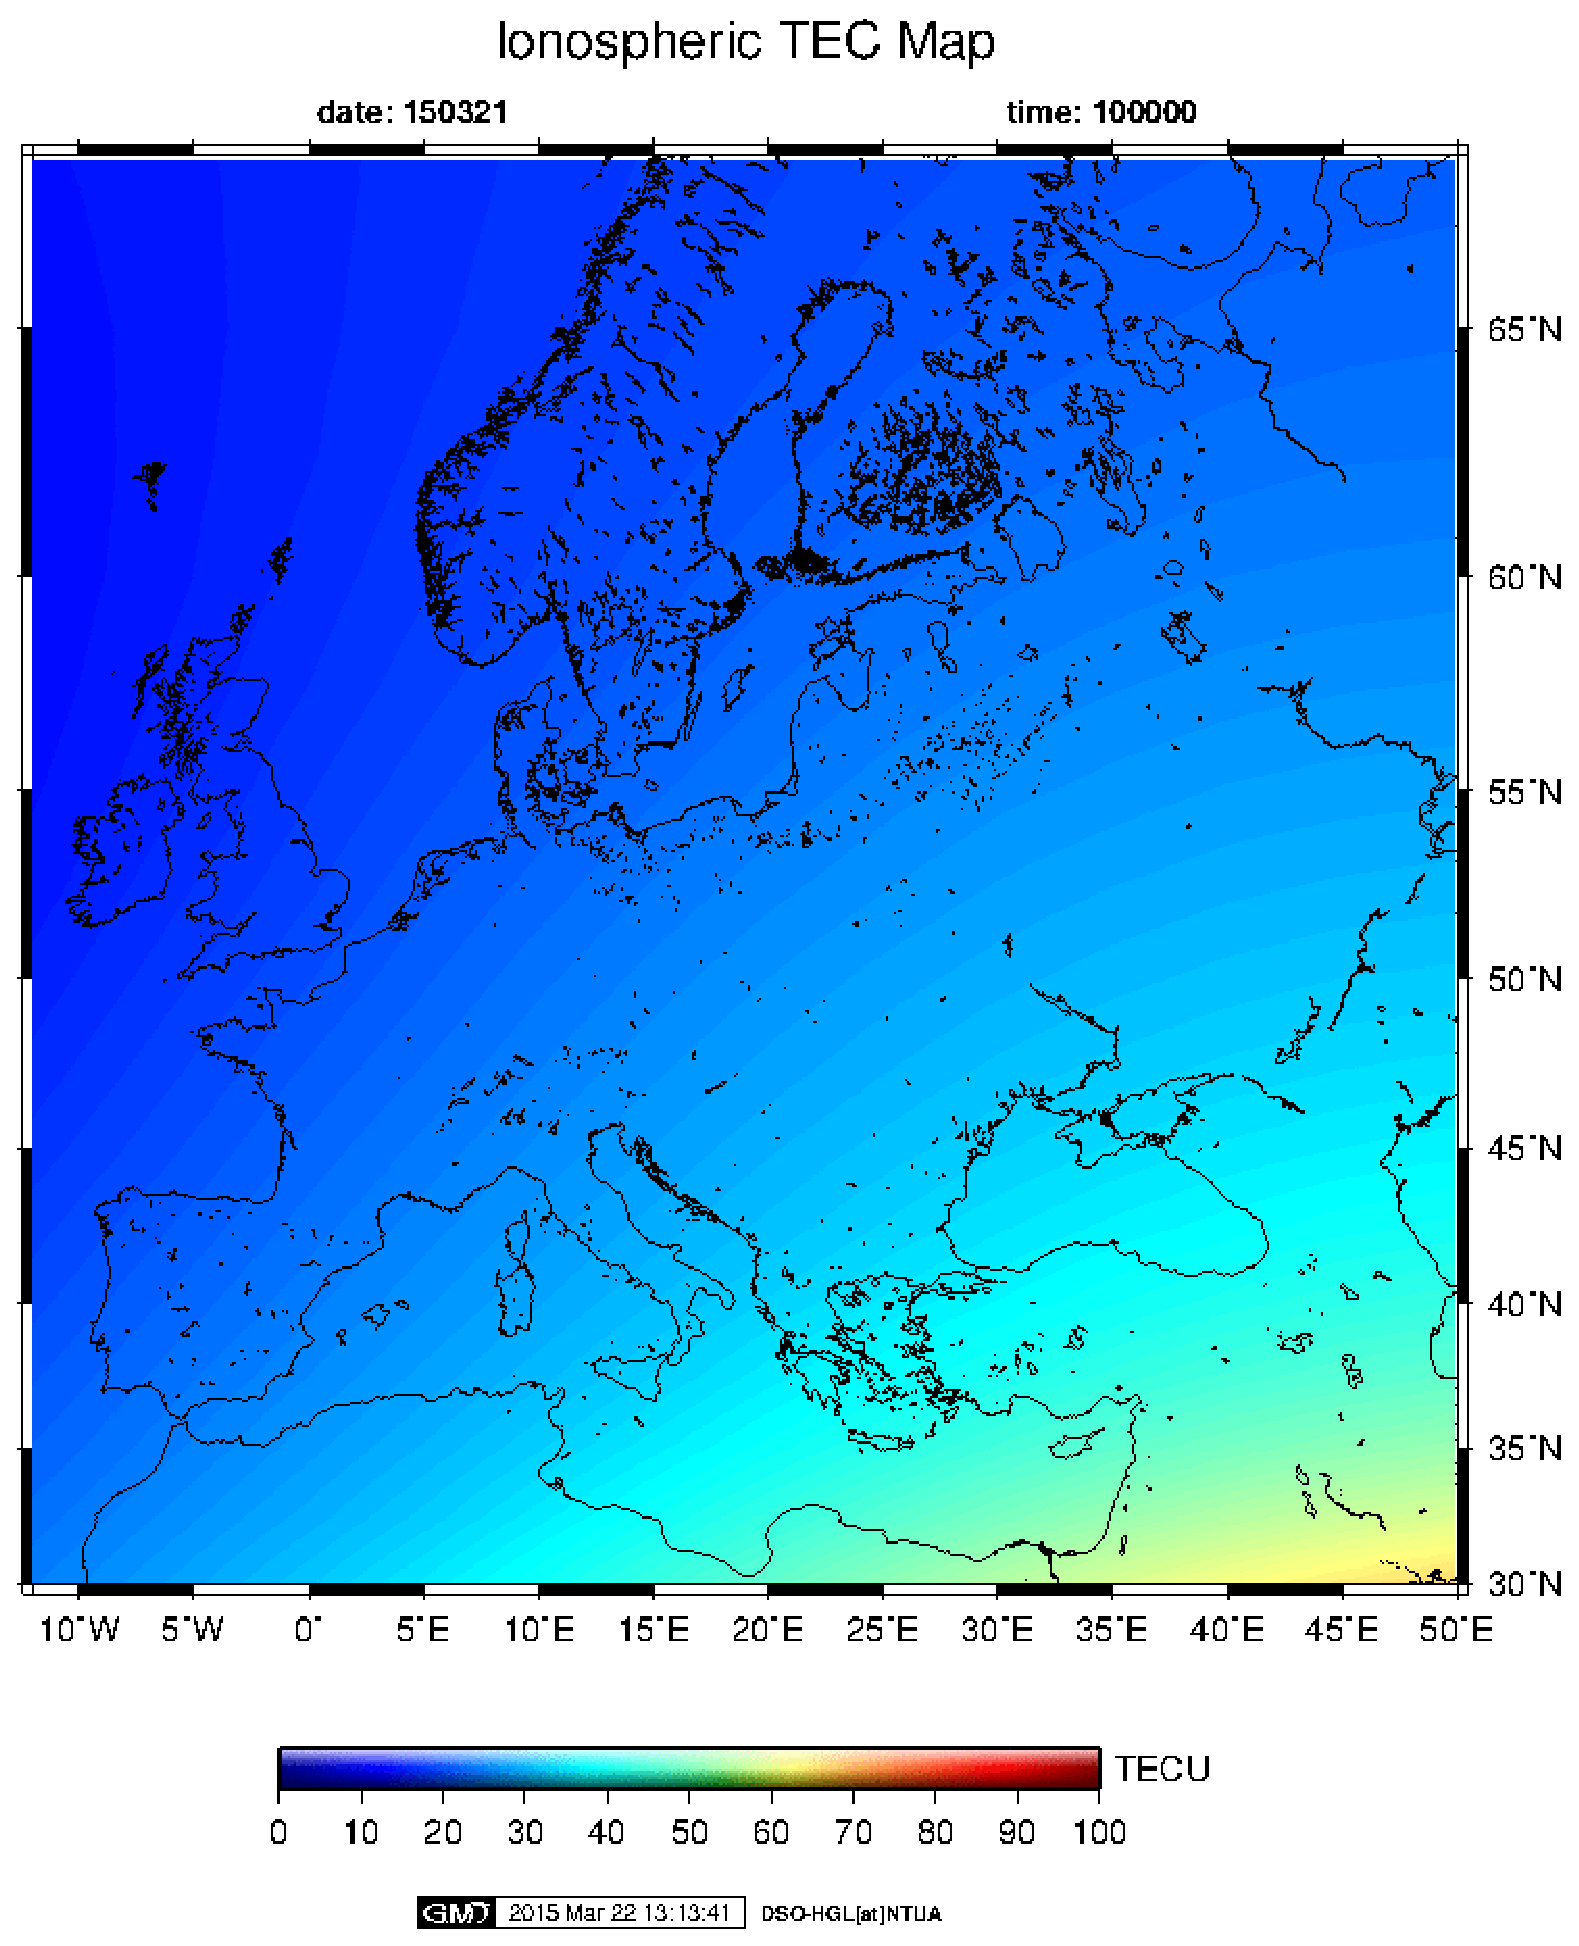
\includegraphics[height=4cm]{img/iono.eps}}};
% %   \pause
%   \node (img2) at (img1.north east) [yshift=-1cm,xshift=2.7cm] {\shadowbox{\color{black!35}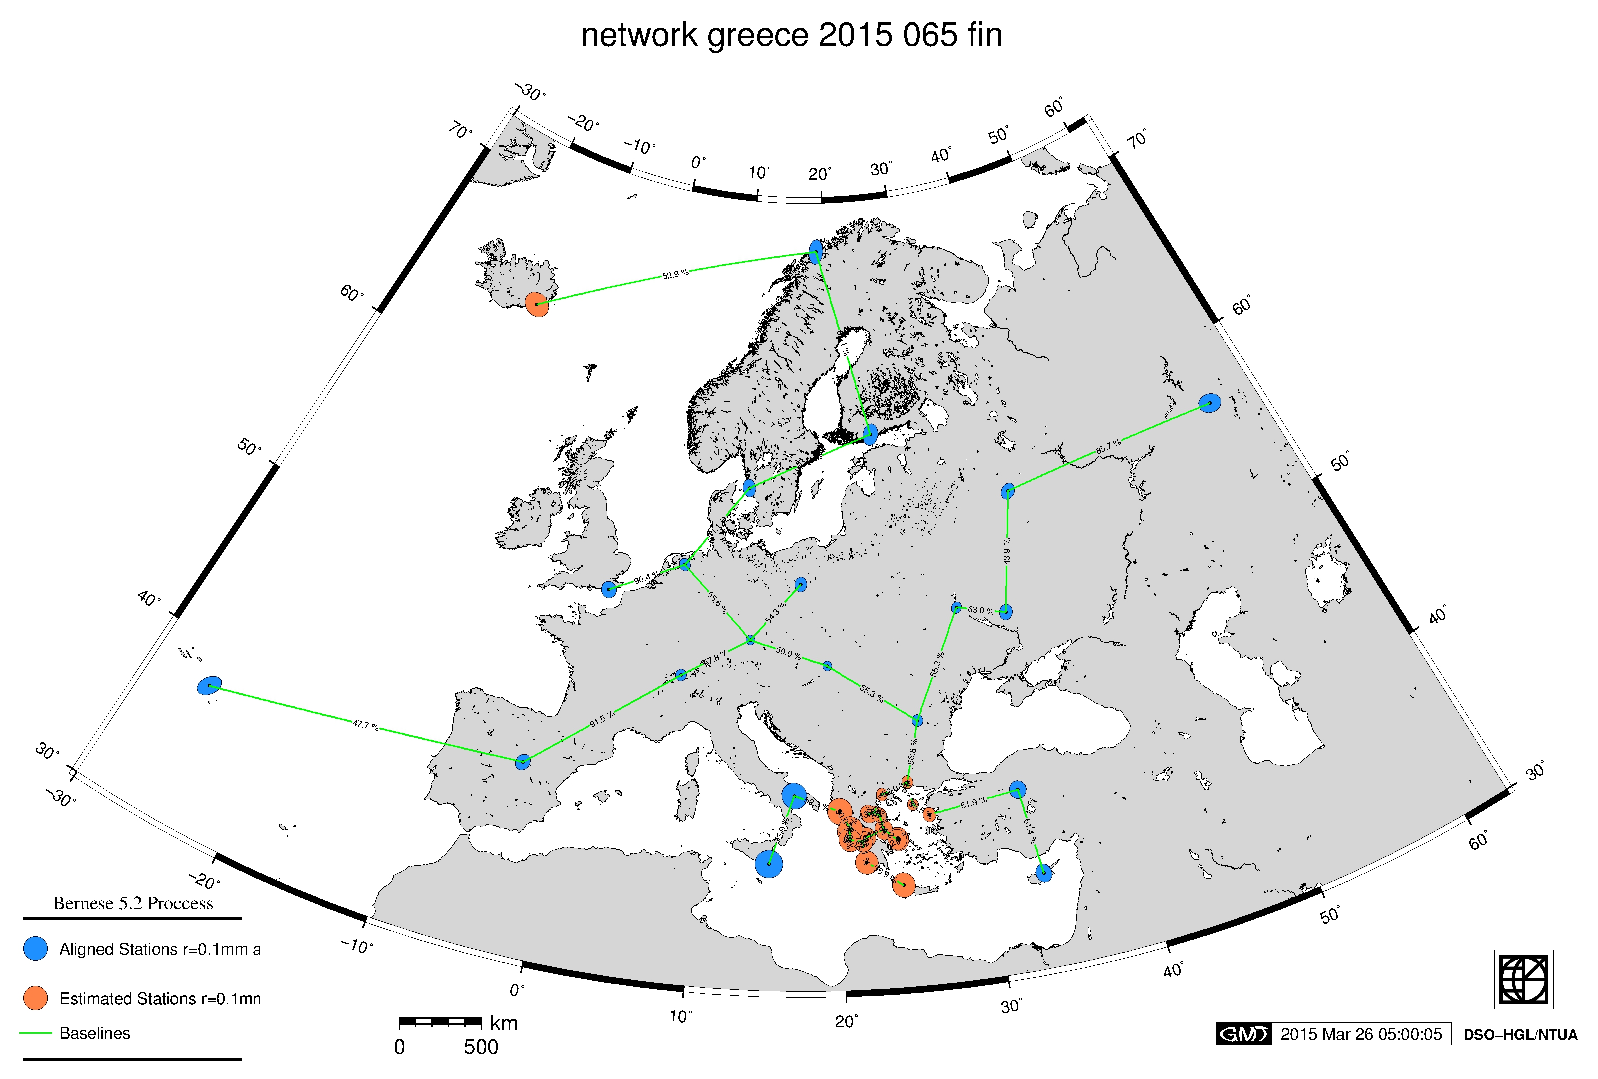
\includegraphics[height=2cm]{img/baseline.eps}}};
% %   \pause
%   \node (img3) at (img2.south) [yshift=-1.5cm,xshift=-.5cm] {\shadowbox{\color{black!35}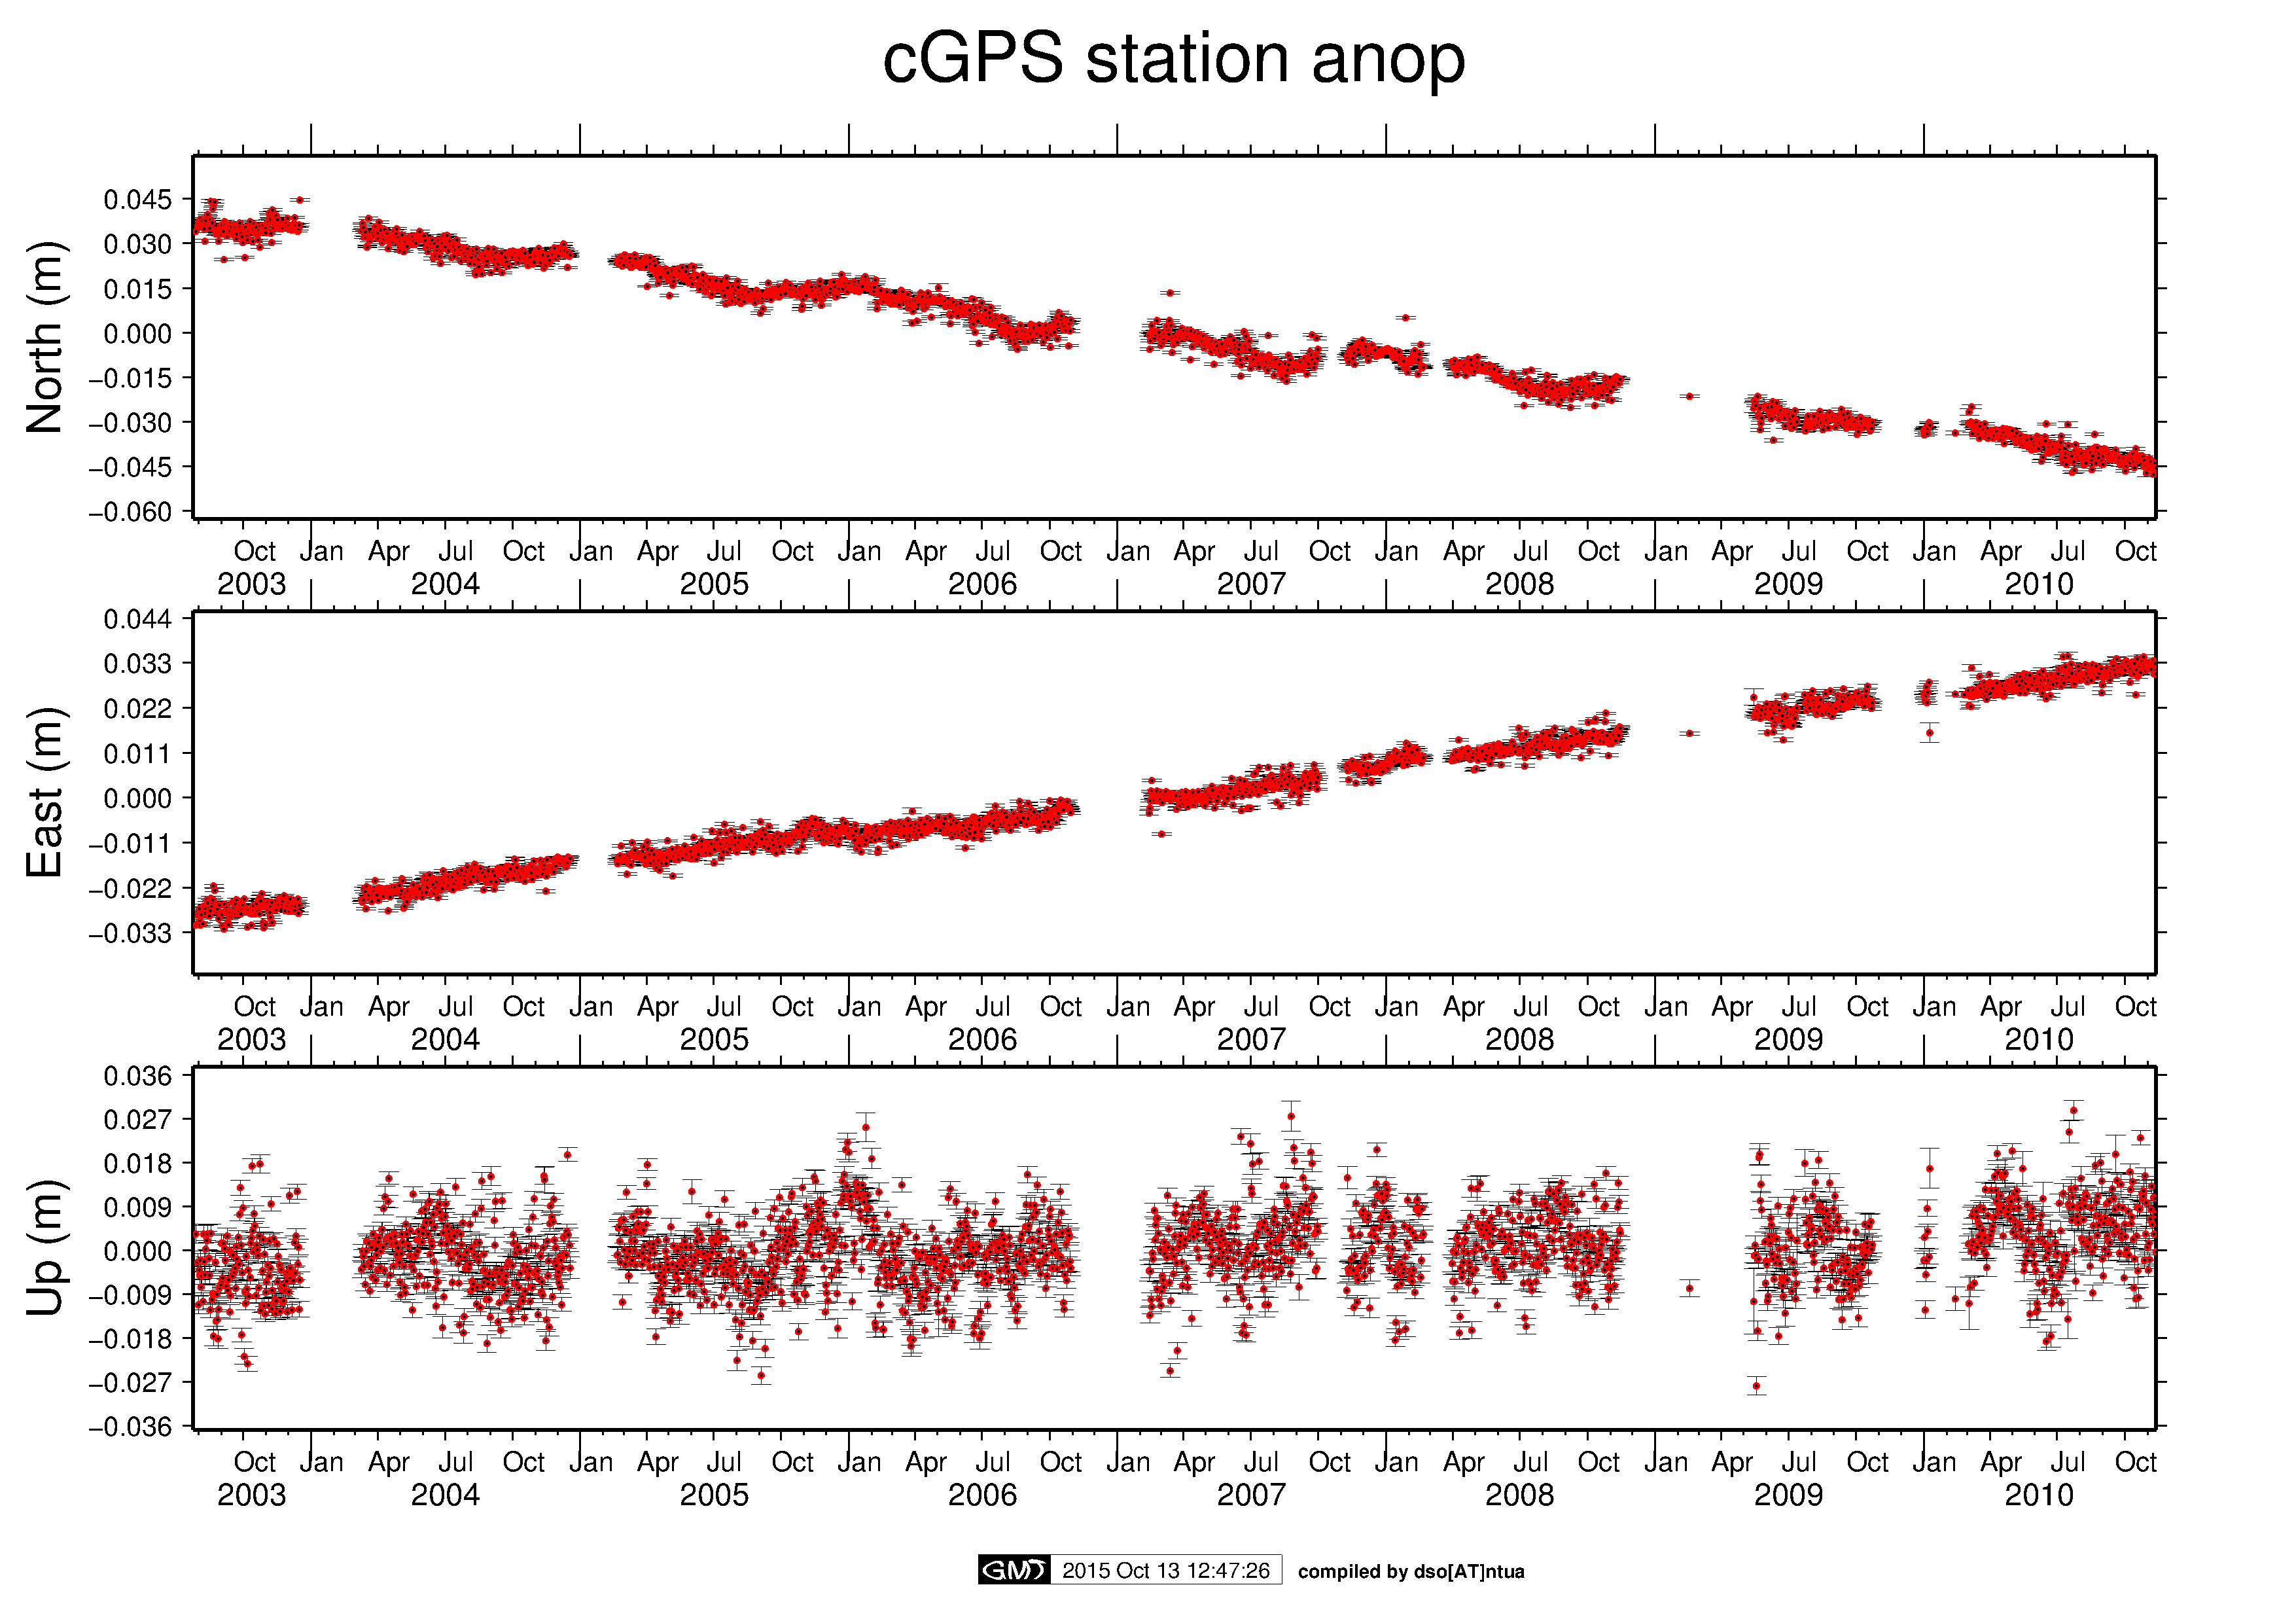
\includegraphics[height=2.6cm]{img/anop-raw.png}}};
% %   \pause
% %   \node (img4) at (img2.south west) [yshift=2cm] {\includegraphics[height=4cm]{img/dsoprint.png}};
% \end{tikzpicture}
% \end{center}
% \end{frame}
% }
% 
% \section{Web Resources}
% 
% \begin{frame}\frametitle{Web Resources}\framesubtitle{Visit, Browse, Interact, Comment}
% \begin{itemize}
%     \item \textbf{Dionysos Satellite Observatory} \url{http://dionysos.survey.ntua.gr/}  %%{http://dionysos.survey.ntua.gr/}
%     \item \textbf{GSAC repository} \url{http://dionysos.survey.ntua.gr/dsoportal/_datacenter/gsacrepos.html} %%{http://dionysos.survey.ntua.gr/dsoportal/\_datacenter/gsacrepos.html}
%     \item \textbf{Ftp site} \url{http://dionysos.survey.ntua.gr/dsoportal/_datacenter/ftpdata.html}  %%{http://dionysos.survey.ntua.gr/dsoportal/\_datacenter/ftpdata.html}
%     \item \textbf{Kefallonia earthquake} \url{http://dionysos.survey.ntua.gr/dsoportal/_projects/supersites/cephalonia/}  %%{http://dionysos.survey.ntua.gr/dsoportal/\_projects/supersites/cephalonia/}
%     \item \textbf{Ionospheric Remote Sensing} \url{http://dionysos.survey.ntua.gr/dsoportal/_projects/IonoRemSens/}  %%{}
% \end{itemize}
% \end{frame}
% 
% \section{Thank you}
\begin{frame}\frametitle{}\framesubtitle{}
    \begin{center}
    Ευχαριστώ για την προσοχή σας !
    \end{center}
%     \begin{figure}
%  \begin{center}
%  \vskip .5cm
%  
\includegraphics[width=.7\textwidth]{../figures/ESPA-EKT-GSRT_Logo-GR.png}
%  \end{center}
% \end{figure}
\end{frame}
% 
\begin{frame}[allowframebreaks]
  \frametitle<presentation>{References}
  \begin{thebibliography}{10}

%  \beamertemplatebookbibitems
% %  \bibitem{Autor1990}
% %    A.~Autor.
% %    \newblock {\em Introduction to Giving Presentations}.
% %    \newblock Klein-Verlag, 1990.
% 
  \beamertemplatearticlebibitems
% 
    %% Bernese
    \bibitem{bpe}
    Dach R., Hugentobler U., Fridez P., Meindl M.
    \newblock Bernese GPS Software Version 5.0
    \newblock {\em Astronomical Institute, University of Bern}, 2007.
% 
%     %% Papoutsis, Santorini
%     \bibitem{papoutsis}
%     Papoutsis I., Papanikolaou X., Floyd M., Ji K. H., Kontoes C., Paradissis D., Zacharis V.
%     \newblock Mapping inflation at Santorini volcano, Greece, using GPS and InSAR
%     \newblock {\em Geophysical Research Letters}, 40(2):267-272, 2013
%     
%     %% papanikolaou
%     \bibitem{papanikolaou}
%      X. Papanikolaou, D. Anastasiou, A. Marinou, V. Zacharis, and D. Paradissis 
%     \newblock Routine Analysis of all available GNSS Stations in Greece: Data, products and preliminary results
%     \newblock {\em  The Volcanic and Geodynamic Field of the South Aegean, International Workshop, 20-22 May, Santorini, Greece}
% 
% 
%     %% Sakkas, Kephalonia
%     \bibitem{sakkas}
%     Sakkas V., Lagios E.
%     \newblock Fault modelling of the early-2014 $\sim$ M6 Earthquakes in Cephalonia Island (W. Greece) based on GPS measurements
%     \newblock {\em Tectonophysics}, Volumes 644–645,184-196, 2015, Pages 184-196
% 
%     %% Diaforoi, sar kephalonia
%     \bibitem{sarkefalonia}
%     Merryman Boncori J.P., Papoutsis I., Pezzo G., Tolomei C., Atzori S., Ganas A., Karastathis V., Salvi S., Kontoes C., Antonioli A.
%     \newblock The February 2014 Cephalonia Earthquake (Greece): 3D Deformation Field and Source Modeling from Multiple SAR Techniques
%     \newblock {\em Seismological Research Letters}, Vol.86(1), 2015
% 
%     %% Unavco GSAC
%     \bibitem{gsac}
%     UNAVCO
%     \newblock GSAC -- Geodetic Seamless Archive Centers: Open-source Software for Geodesy Data Repositories
%     \newblock {\em available at} \url{https://www.unavco.org/software/data-management/gsac/gsac.html}
% 
    %% Unavco IGB08
    \bibitem{igb08}
    P. Rebischung
    \newblock IGb08: an update on IGS08
    \newblock {\em IGSMAIL [6663]} \url{http://igscb.jpl.nasa.gov/pipermail/igsmail/2012/007853.html}, 2012

    %% Unavco vmf1
    \bibitem{vmf1}
    Boehm J., B. Werl, and H. Schuh (2006)
    \newblock Troposphere mapping functions for GPS and very long baseline interferometry from European Centre for
    Medium-Range Weather Forecasts operational analysis data
    \newblock {\em Journal of Geophysical Research}, vol. 111, B02406, 2006
% 
  \end{thebibliography}
\end{frame}

\end{document}